\newcommand{\bo}{\(b\)}

\chapter{\label{chap:gcol}The Graph Colouring Problem}

\section{\label{sec:gcol:background}Background}

The Graph Colouring Problem is a deceptively simple problem in graph theory.  In its most basic form, it is the problem of assigning labels such as colours to the nodes in a graph, such that no two nodes connected by an edge share a colour, usually with the addition of the extra requirement either of finding the minimum number of colours required or only using a number of colours up to some upper bound --- for any graph with \(N\) nodes, it is trivial to colour it using \(N\) colours.  The problem finds applications in many areas, including timetabling, register allocation for compilers, as well as solving Sudoku puzzles (which are in turn a special case of Latin Squares) \cite{Lewis2016}.  The general case is NP-Complete, and thus no polynomial time solution has been found so far (finding one would prove that P = NP), though they have been found for specific forms of graph or particular numbers of colours.  For example, in the case of 3-colouring, the current best known solution takes \(\mathcal{O}(1.3289^n)\) time \cite{Beigel2005}.

% Gheorghe \textit{et al.} presented a \gls{ps} solution to the 3-colouring problem, using communicating \gls{skps} \cite{Gheorghe2013}.  Based on this work, we first discuss in \autoref{sec:gcol:cml} a \gls{cml} implementation of the \gls{skps} solution in \cite{Gheorghe2013}, briefly compare the two approaches and indicate some other \gls{ps} variants we think \gls{cml} might be a good fit with.  We then present in \autoref{sec:gcol:cpsys} a fairly concise single-cell solution to the problem using \gls{ps} with compound terms (\gls{cps} for short -- see \cite{Nicolescu2018} for a detailed background on \gls{cps}), and provide an informal analysis of it.  Lastly, in \autoref{sec:gcol:examples}, we provide examples of the operation of our cP~system on the 3-colour problem, both for a graph that is colourable and one that is not, before concluding in \autoref{sec:gcol:conc}.

% To the best of our knowledge, this is the first time \gls{cps} has been applied to graph colouring, and the first time that a \gls{cml} implementation has been used to simulate the operation of any P~system.

% We wish to emphasise that we do not consider our simulation or \gls{cps} solution to be `superior' to that of Gheorghe \textit{et al.} (though we do think it demonstrates the utility of \gls{cps}), but instead wish to complement theirs and others' work with another alternative.

% \section[Simple Kernel P Systems Solution to the \glsfmtname{gcp-glossary} in \glsfmtname{cml-glossary}][\Gls{skps} Solution to the \gls{gcp} in \gls{cml}]{\label{sec:gcol:cml}Simple Kernel P Systems Solution to the \glsfmtlong{gcp-glossary} in \glsfmtlong{cml-glossary}}

This \namecref{sec:gcol:cml} explores \gls{cml} as another methodology to use for simulating \gls{ps} where communication is involved.  For a first experiment, it implements \citeauthor{Gheorghe2013}'s 3-colouring problem solution from \cite{Gheorghe2013}, as it involves communication between \glspl{compartment} but is relatively low-complexity and thus appears to be suitable for a first attempt at simulating communicating \gls{ps} with \gls{cml}.

The programming language \fsharp{} was used with the library Hopac,\footnote{\url{https://github.com/Hopac/Hopac}} which is modelled on \gls{cml} and follows it closely.\footnote{The final program can be found at \url{https://github.com/jcoo092/acmc2018}}  `Record' types are used to represent the individual \glspl{compartment} described in \cite{Gheorghe2013}.  The program then advances through multiple steps, applying the rules (encoded as functions that operate on the record types) in accordance with \cite{Gheorghe2013}.  Finally, once a solution is found, or found not to be possible, that is communicated to the environment.

Insofar as possible, the implementation follows the algorithm described in \cite{Gheorghe2013} faithfully, and thus perhaps is not optimal in its efficiency, as an idiomatic specification of a Simple Kernel P~system does not necessarily match to the idiomatic or efficient form of an \fsharp{} program.  That is, the program prioritises staying as close to the original \gls{skps} model as possible, rather than adapting to suit the strengths and typical style of \fsharp{}.  Consequently, the efficiency of the program may be worse than it could be otherwise.

\subsection{Simulation Results}
The program's running time on a number of differing graphs were recorded, with red, green and blue as the set of colours with which to colour the graphs.  The desktop computer used for these simulations has a four-core \qty{3.6}{\giga\hertz} Intel Core\textsuperscript{\textregistered} i7-7700 CPU, with \qty{16}{\gibi\byte} of RAM, running Windows 10, build number 10.0.17134.228.  The \fsharp{} programs were compiled and run on .NET Core 2.1.4, while \gls{mecosim} was run on Java version 8, build 1.8.0\_201-b09.

The first simulation used the graph shown in Figure 2 of \cite{Gheorghe2013}, reproduced here as \cref{fig:gcol:gheorghefig2}, which took \qty{2.6}{\second} to process.  In keeping with that paper and following its definition of \(G(N,q)\), where \(G(N,q)\) is used to represent a graph of \(N\) nodes with all other nodes connected only to node \(q\) in a hub-and-spoke formation,\footnote{This is different to the random graphs that are also commonly denoted by this notation.} the graphs \(G(10,1)\) and \(G(10,10)\) (see \cref{fig:gcol:gs}) were also tested, finding that \qty{0.3}{\second} is required for each.  The simulation was also tested using the classic \emph{Petersen graph}, shown in \cref{fig:gcol:petersen}, and found that it too required approximately \qty{0.3}{\second}.

\begin{figure}
    \centering
    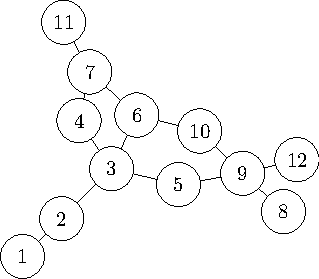
\includegraphics[width=0.65\textwidth]{chapters/gcol/figs/gheorghe-figure-2-figure0.pdf}
    \caption[A reproduction of the graph in Figure 2 of \cite{Gheorghe2013}]{\label{fig:gcol:gheorghefig2}A reproduction of Figure 2 from \cite{Gheorghe2013}.  Although this figure and Figure 2 in \cite{Gheorghe2013} are visually distinct, the graphs are isomorphic.}
\end{figure}

\begin{figure}
    \centering
    \begin{subfigure}[b]{0.35\textwidth}
        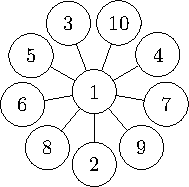
\includegraphics[width=\textwidth]{chapters/gcol/figs/g-10-1.pdf}
        \caption{\label{fig:gcol:g-10-1}\(G(10,1)\)}
    \end{subfigure}
    \hfill
    \begin{subfigure}[b]{0.35\textwidth}
        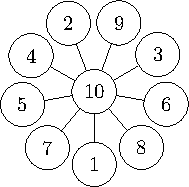
\includegraphics[width=\textwidth]{chapters/gcol/figs/g-10-10.pdf}
        \caption{\label{fig:gcol:g-10-10}\(G(10,10)\)}
    \end{subfigure}
    \caption[Graphs representing \(G(10,1)\) and \(G(10,10)\)]{\label{fig:gcol:gs}Graphs representing (a) \(G(10,1)\) and (b) \(G(10,10)\), as described in \cite{Gheorghe2013}, where the first number represents the size of the graph, and the second number represents the label of the centre node of the graph, with all other nodes connected only to that node.}
\end{figure}

\begin{figure}
    \centering
    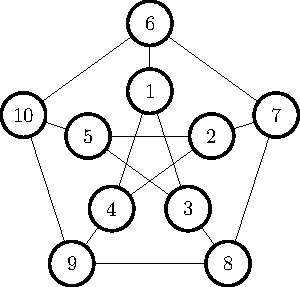
\includegraphics[width=0.45\textwidth]{chapters/gcol/figs/petersen-figure0.pdf}
    \caption[The Petersen Graph]{\label{fig:gcol:petersen}The classic Petersen graph, with nodes labelled 1 to 10.}
\end{figure}

Further simulations were run on complete graphs.  For a complete graph of \(N = 10\), the algorithm again required \qty{0.3}{\second}.  It was then tried on a complete graph of \(N = 20\), but the test had to be aborted after a matter of minutes due to the computer running out of memory.  Running times of \qty{0.83}{\second}, \qty{2.6}{\second}, \qty{8.88}{\second}, \qty{26.6}{\second} and \qty{84}{\second} for \(N = 11, 12, 13, 14\) and \(15\), respectively, were recorded.  Given that significant jumps in memory use were observed while running the larger graphs, it appears that the major cause of the rapid slowdown is likely to do with frequent \adhoc{} memory allocations and de-allocations, though this was not profiled in detail.

\citeauthor{Gheorghe2013} state \cite[p.~828]{Gheorghe2013} that in the latest version of \gls{plingua} at the time of writing, a strategy of eliminating \glspl{compartment} for which there can be no further rule applications is employed.  Using said strategy, results are typically achieved quite quickly.  It has the effect of pruning the search space, and reduces the total running time in some instances to just one-fifth of the running time of the simulation without such dead-\gls{compartment}-elimination.

The \fsharp{} program does not choose which \glspl{compartment} to operate upon in the same fashion, but applying the colour guard on rule \(r_{2,2n+1}\) of the \gls{skps}~system throughout the process results in the pruning of \glspl{compartment} which already contain invalid results and thus can be eliminated safely. Therefore, to achieve the same effect as with \gls{plingua}'s strategy, this guard was used while applying rule \(r_{2,2n+1}\) and the result used to filter out all invalid \glspl{compartment}.  Doing this reduces the evaluation of complete graphs to around 60 milliseconds or slightly more, since every \gls{compartment} in them can always be eliminated once colours have been assigned to four nodes.  It also reduces the running time of \cref{fig:gcol:gheorghefig2} to around \qty{0.25}{\second}, and the Petersen graph, \(G(10,1)\) and \(G(10,10)\) to \qty{0.1}{\second}.

\subsubsection{Comparison with Original Results}

\Cref{tab:gcol:timings} compares the timing results of the simulations reported in \cite{Gheorghe2013}, as well as the results of using \gls{mecosim}\footnote{The latest version of \gls{mecosim} available from \url{http://www.p-lingua.org/mecosim/} as at 10 January 2019 was used.} \cite{Perez-Hurtado2010} to re-run the same simulations locally on the same computer used to time the \fsharp{} solution, with the timing results mentioned above.

\begin{table}
\centering
\begin{tabular}{@{}lcccc@{}}
\toprule
Graph       & \begin{tabular}[c]{@{}c@{}}\gls{plingua}\\ (original)\end{tabular} & \begin{tabular}[c]{@{}c@{}}\gls{plingua}\\ (local)\end{tabular} & CML   & \begin{tabular}[c]{@{}c@{}}CML with\\ pruning\end{tabular} \\ \midrule
Fig. 2 in \cite{Gheorghe2013}      & N/A                                                           & 17.0                                                           & 2.6  & 0.25                                                 \\
Petersen    & N/A                                                           & 1.5                                                       & 0.3  & 0.1                                                       \\
G(10,1)     & 7                                                            & 2.6                                                           & 0.3  & 0.1                                                       \\
G(10,10)    & \textgreater 4 min                             & N/A                                                           & 0.3  & 0.1                                                       \\
Complete 11 & 5                                                            & 0.15                                                           & 0.83 & .06                                                       \\
Complete 12 & 5                                                            & 0.15                                                           & 2.6  & .06                                                       \\
Complete 13 & 5                                                            & 0.15                                                           & 8.88 & .06                                                       \\
Complete 14 & 5                                                            & 0.15                                                           & 26.6 & .06                                                       \\
Complete 15 & 5                                                            & 0.15                                                           & 84   & .06                                                       \\ \bottomrule
\end{tabular}%
\caption[Comparison of recorded timings between \cite{Gheorghe2013} and this work]{Comparison of recorded timings between \cite{Gheorghe2013} and this work.  All measurements are in seconds, unless otherwise stated.  Where more than one result was reported in \cite{Gheorghe2013} for the same graph, the shortest running time has been included here.}
\label{tab:gcol:timings}
\end{table}

Attempts to run the simulation of \(G(10,10)\) in \gls{mecosim} repeatedly failed with an out-of-memory error.  Why this should be the case is uncertain, given that in the other instances, executions of the \gls{mecosim} \gls{skps} simulations achieved lower runtimes than those of \cite{Gheorghe2013}.  The execution of \(G(10,10)\) notwithstanding, the overall improvements in runtime of the \glspl{skps} are likely due to a combination of the computer used locally being more recent and thus likely more powerful, and improvements in the underlying \gls{mecosim} and \gls{plingua} software.

It seems odd, however, that two functionally identical graphs, \(G(10,1)\) and \(G(10,10)\), would have such dramatically different run time behaviours when running in \gls{mecosim} --- seen in both the original and reproduced local results.  This might be due to an unusual performance bug hidden deep within \gls{mecosim}, though this was not investigated further.

These results appear to suggest that the \fsharp{} implementation generally provides superior running time results, though it was not tested on a particularly wide variety of scenarios.  Extrapolating from the collected results, it seems plausible that the scenarios that would result in the longest running time will likely be those that have a moderate level of connectedness in the graph.  Highly connected graphs will likely see many potential paths eliminated early due to frequent occurrences of colour conflicts, while graphs with few connections will have relatively few potential paths to explore.

The \fsharp{} results and those of the \gls{mecosim} simulations are not \emph{completely} comparable, however.  The \fsharp{} solution was programmed directly to follow the \gls{skps} system's rules, whereas the \gls{mecosim} solution was specified as the \gls{skps}~system rules in \gls{plingua}, with the operation of the computer simulation carried out by \gls{mecosim}.  This difference between `\adhoc{}' and `general' simulation means that one would expect to see the \fsharp{} simulation achieve better results from the outset, as overheads that accompany a general simulation implementation can be avoided.\footnote{One could see \adhoc{} as being akin to running a program compiled to native instructions, whereas using a general simulation is similar, in principle, to running a program in an interpreter.  The latter is typically simpler to work with and more portable, but comes with overheads that slow down execution.}  \Gls{mecosim} is an excellent tool, and, combined with \gls{plingua}, it provides a valuable service to the \gls{mc} community in that it allows researchers to validate their systems and \glspl{ruleset} while staying close to their mathematical descriptions, and without having to delve into the details of implementing a given algorithm in code.  See further \cite{Perez-Hurtado2019} for more of a discussion on \adhoc{} and general simulations, and a narrowing of the differences between the two.

Ultimately, this example is relatively trivial and involves little communication, and therefore does not test the use of \gls{cml} significantly.  Much of the operation of the algorithm in fact does not involve communication between different \glspl{compartment}/processing elements at all.  Instead, it is primarily based in the evolution of objects contained within the \glspl{compartment}, with minimal communication between \glspl{compartment} at the end.  While that is highly effective in \gls{ps} \cite{Paun2008}, it would be interesting to see the results of using \gls{cml} for other problems where synchronous communication\footnote{While \gls{cml} uses synchronous communication by default, it is also relatively simple to implement asynchronous communication also using it if desired \cite{Reppy2007}.} is a much bigger part of the evolution of the system.  The experimental results in \cref{chap:median} go some way to investigating this.

In common with most \adhoc{} simulations, while the implementation is reasonably successful, it is not particularly customisable, and the code as written does not comport as precisely to the appearance of the theoretical rules of the \gls{skps}~system as the \gls{plingua} version created for \cite{Gheorghe2013} does.  Neither does the current implementation have any form of verification or invariant detection, as provided by \gls{mecosim} \cite{Perez-Hurtado2010} and Spin \cite{Ben-Ari2008,Lefticaru2011}.

\gls{cml} seems to match to \gls{skps} well, but also looks like it might fit well with \gls{tlps} with symport/antiport \cite{Verlan2005} as well perhaps as \gls{tlps} with Channel States \cite{Song2016}, and Generalized Communicating \gls{ps} with minimal interaction rules \cite{Csuhaj-Varju2011}.  It would also appear to be a good fit for \gls{snps} \cite{Ionescu2006}, though \gls{cml} would probably be `overkill' for \gls{snps}.  In general, any variant of \gls{ps} which heavily uses synchronous communication between different cells/neurons/non-nested membranes/etc. over well-defined channels may be amenable to a \gls{cml} implementation.

Technically, the base form of \gls{cml} would only support symport (\ie{} one-way synchronous communication), but it is fairly simple to build two-way communication on top of it \cite[ch.~6]{Reppy2007}.  No attempt to model other systems has been made yet, however.
% \section{\label{sec:gcol:cpsys}\glsentrytext{cps} solution to the \glsentrytext{gcp}}
In the \gls{cml} simulation of the problem, most of the work, in fact, is performed by the instantiation of new objects, rather than communication.  Thus, the problem appears to be an excellent fit to the pre-existing formulation of \gls{cps} \cite{Nicolescu2018}.

This solution assumes a graph with at most one edge between nodes (i.e. there are not two or more edges between the same two nodes), and that there are no edges leading from a node back to itself.  Further, it takes as given inputs to the process conceptual finite sets \(V \subset \mathbb{N}\) representing the nodes of the graph\footnote{In fact, any finite set of arbitrary symbols could be used, but this discussion is restricted to the natural numbers for ease of reading.}; \(E \subseteq \{(i,j)~|~i, j \in V, i \neq j \}\) representing the edges of the graph; and \(K\) representing the chosen colours, where \(K\) contains whatever representation of the desired colours is considered appropriate.

Based on these definitions, for the purposes of the remainder of this \namecref{chap:gcol}, \(|K|\) is defined to be the number of colours used in the current problem, \(|V|\) the number of nodes in the graph under consideration for the current problem and \(|E|\) the number of edges in the graph.

\subsection{Pseudocode for our parallel algorithm}
The logical operation of the system, as carried out using the rules described in detail at \cref{sec:gcol:rules}, can be demonstrated with a pseudocode representation, as shown in \cref{code:gcol:graphcol}.

% \begin{algorithm}
% \DontPrintSemicolon
% \SetKwFunction{Choose}{choose}
% \SetKwFunction{Dom}{Dom}
% \SetKwFunction{Graphcolouring}{Graph Colouring}
% \KwIn{\(V\), \(E\), \(K\)}
% \KwOut{A valid colouring, or an indication no valid colouring is possible}
% \Begin{
% \Choose{\(s \in V\), \(c \in K\)}\;
% \KwRet{\Graphcolouring{\(V\), \(E\), \(K\), \(1\), \(\{\{(s, c)\}\}\)}} \label{li:gcol:endofsmaller}
% }

% \hrulefill

% \KwIn{\(V\), \(E\), \(K\), \(i\), \(B\)}
% \KwOut{A valid colouring, or an indication no valid colouring is possible}
% \Begin{
% \If{\label{li:gcol:iflgreaterthanv} \(i = |V|\)} {
%     \Choose{\(m \in B\)}\;
%     \KwRet{\(m\)}    \label{li:gcol:returnsuccess}
% }
% \(B' \gets \emptyset\)\;
% \For{ \(m \in B,~x \in \Dom{m},~y \in V \setminus \Dom{m},~ d \in K \)}{    \label{li:gcol:makebstart}
%     \If{\((x,y) \in E ~ \land \not\exists(x',y) \in E,~(x',d) \in m\)}{
%         \(B' \gets B' \cup \{m \cup \{ (y,d) \} \}\)\;   \label{li:gcol:makebfinish}
%     }
% }
% \eIf{ \label{li:gcol:fail1} \(B' = \emptyset\) }
%   {
%         \KwRet{\(\emptyset\)}  \label{li:gcol:fail2}}
%     {
%         \KwRet{\Graphcolouring{\(V\), \(E\), \(K\), \(i + 1\), \(B'\)}\label{li:gcol:recurse}}
% }}
% \caption[Pseudocode representation of the algorithm performed by the \glspl{cps} rules in \cref{ruleset:gcol:rules}]{\label{code:gcol:graphcol}Pseudocode representation of the algorithm performed by the \glspl{cps} rules in \cref{ruleset:gcol:rules}.  This employs a doubly defined tail-recursive function approach, where the algorithm begins with the upper function supplied only with the details of the graph and colours, but uses the lower function with further arguments to perform most of the processing.}
% \end{algorithm}

\begin{algorithm}
\DontPrintSemicolon
\SetKwFunction{Choose}{choose}
\SetKwFunction{Dom}{Dom}
\SetKwFunction{Graphcolouring}{Graph Colouring}
\KwIn{\(V\), \(E\), \(K\)}
\KwOut{A valid colouring, or an indication no valid colouring is possible}
\Begin{
\Choose{\(s \in V\), \(c \in K\)}\;
\KwRet{\Graphcolouring{\(V\), \(E\), \(K\), \(\{\{(s, c)\}\}\)}} \label{li:gcol:endofsmaller}
}

\hrulefill

\KwIn{\(V\), \(E\), \(K\), \(B\)}
\KwOut{A valid colouring, or an indication no valid colouring is possible}
\Begin{
\If{\label{li:gcol:iflgreaterthanv} \(V = \emptyset\)} {
    \Choose{\(m \in B\)}\;
    \KwRet{\(m\)}    \label{li:gcol:returnsuccess}
}
\(B' \gets \emptyset\)\;
\For{ \(m \in B,~x \in \Dom{m},~y \in V \setminus \Dom{m},~ d \in K \)}{    \label{li:gcol:makebstart}
    \If{\((x,y) \in E ~ \land \not\exists(x',y) \in E,~(x',d) \in m\)}{
        \(B' \gets B' \cup \{m \cup \{ (y,d) \} \}\)\;   \label{li:gcol:makebfinish}
    }
}
\eIf{ \label{li:gcol:fail1} \(B' = \emptyset\) }
   {
        \KwRet{\(\emptyset\)}  \label{li:gcol:fail2}}
    {
        \KwRet{\Graphcolouring{\(V\), \(E\), \(K\), \(B'\)}\label{li:gcol:recurse}}
}}
\caption[Pseudocode representation of the algorithm performed by the \glspl{cps} rules in \cref{ruleset:gcol:rules}]{\label{code:gcol:graphcol}Pseudocode representation of the algorithm performed by the \glspl{cps} rules in \cref{ruleset:gcol:rules}.  This employs a doubly defined tail-recursive function approach, where the algorithm begins with the upper function supplied only with the details of the graph and colours, but uses the lower function with further arguments to perform most of the processing.}
\end{algorithm}

In our notation, \(m\) is a partial functional relation to \texttt{Dom}(m); \texttt{Dom}(m) is a partial spanning tree over the graph; \((x, c) \in m\) if and only if \(c\) is the colour of node \(x\);  and \(B\) is the set of all partial functional relations built up so far.

The system works by starting with the colours and graph under consideration, then building up, in a maximally-parallel fashion, a collection of objects which represent all validly coloured partial spanning trees of the graph.  Eventually, once full spanning trees have been constructed, one is chosen at random and its colouring output to the environment.  Or, if no valid colouring is possible, the system will detect that by the complete absence of any partial spanning tree, and signal to the environment that no appropriate colouring is possible.  The conceptual spanning trees are built following all possible tree edges, but checking that all new frond edges do not invalidate the colouring.

Note that while this algorithm is guaranteed to return a valid colouring if one is possible, there is \emph{no} guarantee as to precisely which valid colouring will be selected.  This \namecref{sec:gcol:cpsys} assumes that all potential colourings are equally desirable, and makes no provision for specifying that certain nodes must be coloured from a subset of the available colours.

\subsection{\label{sec:gcol:sysinit}\Glsfmtlongpl{cps} Initialisation}
System construction begins with a \gls{tlc} containing the functor \(V' = \cpset{\cpfunc{v}{\cpfunc{n}{i}} ~|~i \in V}\), which contains the labels of the nodes in \(V\); a set \(E' \subseteq \cpset{\cpfunc{e}{\cpfunc{n}{i} \, \cpfunc{n}{j}} ~|~(i,j) \in E}\) representing the edges of the graph; a starting node \(\cpfunc{s}{h}\) where \(h \in V\) is an arbitrary node label; and a set \(K' = \cpset{\cpfunc{k}{\kappa} ~|~ \kappa \in K}\) of  the potential colours.  In the case of the three-colour problem, it might look like \(K' = \cpset{\cpfunc{k}{r}, \cpfunc{k}{g}, \cpfunc{k}{b}}\). Using separate colour symbols in this fashion means that the algorithm can operate as a \(|K|\)-colour problem, without any other modification.

While colours are represented here as separate symbols for legibility, they can, in fact, be represented equivalently by natural numbers because each colour symbol is contained within a \(k\) functor --- one simply need fill each functor with the appropriate number of the counting symbol to represent the desired different colours.  E.g. \(r\) might be represented by one copy of the unary digit, \(\cpundig\), \(g\) by two and \(b\) by three, i.e. \(r = \cpfunc{k}{\cpundig}\), \(g = \cpfunc{k}{\cpundig^2}\) and \(b = \cpfunc{k}{\cpundig^3}\).  The same is true of the edges.  This means that, in fact, the system requires no extra symbols in its alphabet to represent the colours and edges of a given problem --- it merely re-uses atoms (see further in \cref{sec:gcol:notation}).

\subsection{\label{sec:gcol:notation}\Glsfmtlongpl{cps} Notation}
% \[
% cP\Pi(T, A, O, R, S, s_0)
% \]

% \(T\) is the set of \gls{tlc}s at the start of the evolution of the system; \(A\) is the alphabet of the system; \(O\) is the set of multisets of initial objects in the \gls{tlc}s; \(R\) is the set of rulesets for each \gls{tlc}, \(S\) is the set of possible states of the system, and \(s_0 \in S\) is the starting state of the system. Further, \(|T| = |O| = |R|\).

% \[
% cP\Pi(\{\sigma_1\}, A, \{O_1\}, \{r_1\}, S, s_1)
% \] where the set \(T = \{\sigma_1\}\) is the single \gls{tlc} of the system; \(A = \{b, c, e,\allowbreak l,\allowbreak m,\allowbreak n, s, v, k\} \allowbreak \cup \{\cpundig\}\) is all potential atoms, functors and other symbols of the system (\(\cpundig\) is used here as the counting symbol representing natural numbers); \(O_1 = \{s(h)\} \cup V' \allowbreak \cup E' \allowbreak \cup K'\) is the multiset of initial objects contained within \(\sigma_1\), where \(h\) is an arbitrarily chosen member of \(V\); \(R = \{r_1\}\) is the ruleset in \cref{ruleset:gcol:rules}; \(S = \{s_1, s_2, s_3, s_4\}\) is the potential states of the system; and \(s_1\) is the initial state of the system.

% In accordance with the \gls{cps} definition of \cref{sec:cps:formaldescriptions}, the \gls{gcp} \glspl{cps} can be formalised as \cptuple{g-col}{\cpset{\sigma_1}}{\cpset{b, c, e,\allowbreak l,\allowbreak m,\allowbreak n, s, v, k, \cpundig}}{\cpset{O_1}}{\cref{ruleset:gcol:rules}}{\cpset{s_1, s_2, s_3, s_4}}{s_1} where: the set \(T = \cpset{\sigma_1}\) is the single \gls{tlc} of the system; \(A = \cpset{b, c, e,\allowbreak l,\allowbreak m,\allowbreak n, s, v, k, \cpundig}\) is all potential atoms, functors and other symbols of the system; \(O_1 = \cpset{\cpfunc{s}{h}} \cup V' \allowbreak \cup E' \allowbreak \cup K'\) is the multiset of initial objects contained within \(\sigma_1\), where \(h\) is an arbitrarily chosen member of \(V\); \(R =\) \cref{ruleset:gcol:rules}.%; \(S = \cpset{s_1, s_2, s_3, s_4}\) is the potential states of the system; and \(s_1\) is the initial state of the system.

In accordance with the \gls{cps} definition of \cref{sec:cps:formaldescriptions}, the \gls{gcp} \glspl{cps} can be formalised as \cptuple{g-col}{\cpset{\sigma_1}}{\cpset{b, c, e,\allowbreak i,\allowbreak m,\allowbreak n, s, v, k, \cpundig}}{\cpset{O_1}}{\cref{ruleset:gcol:rules}}{\cpset{s_1, s_2, s_3, s_4}}{s_1} where: \(\sigma_1\) is the single \gls{tlc} of the system and \(O_1 = \cpset{\cpfunc{s}{h}} \cup V' \allowbreak \cup E' \allowbreak \cup K'\) is the multiset of initial objects contained within \(\sigma_1\), where \(h\) is an arbitrary member of \(V\).


\subsection{\label{sec:gcol:rules}Rules}

% \begin{cprulesetfloat}
% \begin{cpruleset}

%     \cprule{s_1}{\cpfunc{v}{\cpfunc{n}{S}Z}}\cponce{s_2}{\cpfunc{b}{\cpfunc{i}{\cpundig} \; \cpfunc{m}{\cpfunc{n}{S} \, \cpfunc{c}{C}} \; \cpfunc{v}{Z}} \; \cpfunc{i}{\cpundig}}
%     \cppromoter{\cpfunc{k}{C}}
%     \cppromoter{\cpfunc{s}{S}}
    
%     \cprule{s_2}{\cpfunc{b}{\cpfunc{i}{\cpdiscard} \; M \; \cpfunc{v}{\cpempty}}}\cponce{s_3}{\cpsend{M}{env}}
    
%     \cprule{s_2}{}\cpmaxpar{s_2}{\cpfunc{b}{\cpfunc{i}{I\cpundig} \; \cpfunc{m}{\cpfunc{n}{X} \, \cpfunc{c}{C}} \; \cpfunc{m}{\cpfunc{n}{Y} \, \cpfunc{c}{D}} \; M \; \cpfunc{v}{Z}}}
%     \cppromoter{\cpfunc{b}{\cpfunc{i}{I} \; \cpfunc{m}{\cpfunc{n}{X} \, \cpfunc{c}{C}} \; M \; \cpfunc{v}{\cpfunc{n}{Y}Z}}}
%     \cppromoter{\cpfunc{e}{\cpfunc{n}{X} \, \cpfunc{n}{Y}}}
%     \cppromoter{\cpfunc{k}{D}}
%     % \cpinhibitor{\{ \cpfunc{e}{\cpfunc{n}{X'} \, \cpfunc{n}{Y}} \land \cpfunc{m}{\cpfunc{n}{X'} \, \cpfunc{c}{D}} \}}
%     \cpinhibitor{\cpfunc{e}{\cpfunc{n}{X'} \, \cpfunc{n}{Y}} \lor \neg ~ \cpfunc{m}{\cpfunc{n}{X'} \, \cpfunc{c}{D}}}
    
%     \cprule{s_2}{\cpfunc{b}{\cpfunc{i}{I} \, \cpdiscard}}\cpmaxpar{s_2}{}
%     \cppromoter{\cpfunc{i}{I}}
    
%     \cprule{s_2}{}\cponce{s_4}{}
    
%     \cprule{s_2}{\cpfunc{i}{I}}\cponce{s_2}{\cpfunc{i}{I\cpundig}}

% \end{cpruleset}
% \caption[\gls{cps} rules for the \glsentrytext{gcp}]{\label{ruleset:gcol:rules}A completely generic \gls{cps} ruleset for solving the \gls{gcp}}
% \end{cprulesetfloat}

\begin{cprulesetfloat}
\begin{cpruleset}

    \cprule[rule:gcol:rules:init]{s_1}{\cpfunc{v}{\cpfunc{n}{S}Z}}\cponce{s_2}{\cpfunc{b}{\cpfunc{m}{\cpfunc{n}{S} \, \cpfunc{c}{C}} \; \cpfunc{v}{Z}} \; }
    \cppromoter{\cpfunc{k}{C}}
    \cppromoter{\cpfunc{s}{S}}
    
    \cprule[rule:gcol:rules:endsucc]{s_2}{\cpfunc{b}{M \; \cpfunc{v}{\cpempty}}}\cponce{s_3}{\cpsend{M}{env}}
    
    \cprule[rule:gcol:rules:loop]{s_2}{}\cpmaxpar{s_2}{\cpfunc{b}{\cpfunc{m}{\cpfunc{n}{X} \, \cpfunc{c}{C}} \; \cpfunc{m}{\cpfunc{n}{Y} \, \cpfunc{c}{D}} \; M \; \cpfunc{v}{Z}}}
    \cppromoter{\cpfunc{b}{\cpfunc{m}{\cpfunc{n}{X} \, \cpfunc{c}{C}} \; M \; \cpfunc{v}{\cpfunc{n}{Y}Z}}}
    \cppromoter{\cpfunc{e}{\cpfunc{n}{X} \, \cpfunc{n}{Y}}}
    \cppromoter{\cpfunc{k}{D}}
    % \cpinhibitor{\{ \cpfunc{e}{\cpfunc{n}{X'} \, \cpfunc{n}{Y}} \land \cpfunc{m}{\cpfunc{n}{X'} \, \cpfunc{c}{D}} \}}
    \cpinhibitor{\cpfunc{e}{\cpfunc{n}{X'} \, \cpfunc{n}{Y}} \lor \neg ~ \cpfunc{m}{\cpfunc{n}{X'} \, \cpfunc{c}{D}}}
    
    \cprule[rule:gcol:rules:loopclean]{s_2}{\cpfunc{b}{\cpdiscard}}\cpmaxpar{s_2}{}
    % \cppromoter{\cpfunc{i}{I}}
    
    \cprule[rule:gcol:rules:endfail]{s_2}{}\cponce{s_4}{}
    
    % \cprule{s_2}{\cpfunc{i}{I}}\cponce{s_2}{\cpfunc{i}{I\cpundig}}

\end{cpruleset}
\caption[\gls{cps} rules for the \glsentrytext{gcp}]{\label{ruleset:gcol:rules}A completely generic \gls{cps} ruleset for solving the \gls{gcp}}
\end{cprulesetfloat}

The rules are presented in \cref{ruleset:gcol:rules}.  The solution consists of six rules, which are invariant to the graph under consideration, and are listed in \emph{weak priority order}.  They are explained below:

\subsubsection{Description of rules}

\begin{enumerate}
\item This rule begins system evolution.  It converts the setup functor \(v\) into a functor \bo{}, which is used further to instantiate new objects with the possible colourings of the system.  It merely selects the node specified by the supplied \(s\) term, and assigns a colour at random.

The \bo{} object holds an \(i\) functor which keeps track of which iteration a given \bo{} belongs to; a multiset of \(m\) functors which track nodes and their assigned colours in a potential solution; and a \(v\) functor which continues to track the reducing unexplored nodes of the graph.

A separate global \(i\) functor is also instantiated at this point, which tracks the current iteration number of the system and which is used in later rules.  This rule begins in state \(s_1\) and ends in state \(s_2\).  This rule corresponds to the upper \texttt{Graph Colouring} function in \cref{code:gcol:graphcol}.

\item This rule is one of the potential end points of the evolution of the system.  If there are no further remaining nodes to explore, i.e. the \bo{} objects have empty \(v\) functors, then one of the \bo{}s is selected at random and the set \(M\) of \(m\) functors within said \bo{} which contain a solution to the colouring problem is output to the environment.  This rule begins in state \(s_2\) and ends in state \(s_3\).  State \(s_3\) is used to indicate to the environment that a solution has been found and the evolution of the system has terminated.  The change in state means that no other rule can be applied if this rule is applied.  This rule corresponds to \crefrange{li:gcol:iflgreaterthanv}{li:gcol:returnsuccess} of the lower \texttt{Graph Colouring} function in \cref{code:gcol:graphcol}.

\item This rule is arguably the heart of the process, and runs in maximally-parallel mode --- meaning that every possible exploration from the currently extant \bo{} objects is performed simultaneously.  In each application, for every pre-existing \bo{} object, new ones are generated with a random colouration assigned to an unexplored node, so long as there exists an edge between those nodes in the graph \emph{and} the selected colours are not the same \emph{and} there does not already exist another \(m\) object within the current \bo{} object that represents another node connected to the newly chosen node with the same colour.  It also increments the iteration counter within the \bo{} object.  This rule begins in state \(s_2\) and ends in state \(s_2\).  This rule corresponds to \crefrange{li:gcol:makebstart}{li:gcol:makebfinish} of the lower \texttt{Graph Colouring} function in \cref{code:gcol:graphcol}.

The interaction of the \(v\) objects in the output and the first promoter work in the same fashion as \(y \in V \setminus \texttt{Dom}(M)\) in the pseudocode of \cref{code:gcol:graphcol}.  That is, this rule selects an \(n\) inside the given \bo{}'s \(v\), but naturally avoids selecting an \(n\) that is already used in one of the \bo{}'s \(m\)s because they have already been removed from \(v\).

\item This rule is a `cleaning' rule, which removes all extant \bo{} objects with the current iteration count, thus keeping the working space relatively clean.  Recall that in \gls{ps}, rules are applied top-to-bottom in a  weak priority order.  This means that, while this rule will eliminate the \bo{} objects used by \cpruleref{rule:gcol:rules:loop} to instantiate the next generation, said objects will not be eliminated until immediately after the application of \cpruleref{rule:gcol:rules:loop} and thus the two rules do not cause conflicts.  This rule begins in state \(s_2\) and ends in state \(s_2\).

The operation of this rule occurs implicitly in the pseudocode, and does not have corresponding lines.  There is no reference to the current set of \bo{}s, \(B\), carried forward into the next call of the pseudocode function.  Instead, \(B\) is replaced with \(B'\) for the next execution of the function, and \(B\) will be cleaned up by the system in whichever way it clears away objects once all references to them have been dropped.

% \item This rule is the other possible termination rule.  It merely transitions to state \(s_4\), which is used to signal to the environment that no solution is possible.  The key to this rule is that, because it transitions to state \(s_4\), it is only applicable if none of the prior rules are.  This effectively means that it can only apply if all \bo{} objects have been removed from the system (because the presence of at least one \bo{} would mean that one of the prior rules will apply), indicating that every possible combination explored so far has already found a colouring conflict and thus there is no possible valid solution.  This rule begins in state \(s_2\) and ends in state \(s_4\).  This rule corresponds to lines \ref{li:gcol:fail1}-\ref{li:gcol:fail2} of the lower \texttt{Graph Colouring} function in \cref{code:gcol:graphcol}.

\item This rule is the other possible termination rule.  It merely transitions to state \(s_4\), which is used to signal to the environment that no solution is possible.  The key to this rule is that, because it transitions to state \(s_4\), it is only applicable if none of the prior rules are.  This effectively means that it can only apply if all \bo{} objects have been removed from the system (because the presence of at least one \bo{} would mean that one of the prior rules will apply), indicating that every possible combination explored so far has already found a colouring conflict and thus there is no possible valid solution.  This rule begins in state \(s_2\) and ends in state \(s_4\).  This rule corresponds to \crefrange{li:gcol:fail1}{li:gcol:fail2} of the lower \texttt{Graph Colouring} function in \cref{code:gcol:graphcol}.

% \item This rule merely increments the global iteration counter.  It is placed last so that the termination rules can trigger before it, as otherwise it will always be applicable while the system is in state \(s_2\).  This rule begins in state \(s_2\) and ends in state \(s_2\), and thus is applied simultaneously with rules 3 and 4.  This rule is implemented in the successive recursive calls of the lower \texttt{Graph Colouring} function in \cref{code:gcol:graphcol} at line \ref{li:gcol:recurse}.  As part of the recursive call the value for \(i\) in the next call is given as the current value of \(i\) plus one, i.e. \(i\) is incremented as part of the function call.
\end{enumerate}

\subsubsection{Definition of terms}
\paragraph{Atoms}
\begin{description}
\cptermdef{\cpempty}{The standard \gls{cps} ``empty'' term symbol.}
% \cptermdef{\cpundig}{The \gls{cps} unary digit.}
\end{description}

\paragraph{Functors}
\begin{description}
\cptermdef{b}{Node exploration term.  This is a collection term, which holds information pertaining to the iteration at which the term was generated, the nodes explored so far on this path and the colours assigned to each node, and the remaining unexplored nodes in the graph.}
\cptermdef{c}{Colouring assignment term.  Records the colour assigned to a node for a particular exploration}
\cptermdef{e}{Edge node.  Lists two locations in the graph, if they have an edge connecting them.}
\cptermdef{k}{Colour term.  Stores one of the colours potentially to be used in colouring the graph under study.}
% \cptermdef{i}{Iteration counter.  Counts how many steps there have been so far in the system's evolution.}
\cptermdef{m}{Explored node term.  Records a node which has been visited in this particular exploration of the graph, and which colour the node was assigned.}
\cptermdef{n}{Node term.  Merely records the label of a node.  Used as part of other terms in the rules.}
\cptermdef{s}{Starting node.  Stores the label of the intended root node of the exploration of the graph.}
\cptermdef{v}{Unexplored nodes term.  Holds \(n\) terms with the labels of all nodes in the graph as yet unexplored in that particular exploration of the graph.}
\end{description}

\paragraph{States}
\begin{description}
\cptermdef{s_1}{System starting state.  The node in the \(s\) term is given a random colouring, and exploration of the graph begins.}
\cptermdef{s_2}{Main loop state.  All exploration of the graph and assignation of potential colours to nodes occurs in this state.}
\cptermdef{s_3}{Result state.  The system ends in this state if a valid colouring has been found.}
\cptermdef{s_4}{Negative result state.  The system ends in this state if no valid colouring is possible.}
\end{description}

\subsection{\label{sec:gcol:termination}Termination and Correctness}
The behaviour of the system in regard to termination and correctness is examined below.  The discussion in this \namecref{sec:gcol:termination} assumes that the number of steps taken is tracked in a variable \(i\).  No such subcell appears in \cref{ruleset:gcol:rules} because the rules make no use of the step number.

\begin{lemma}\label{lemma:gcol:grow}
All \bo{} objects present in the \gls{tlc} hold a monotonically growing set \(M\) of \(m\) functors, which represent validly coloured partial spanning trees of the whole graph, and at step \(i \leq |V|\) in the evolution of the system, each partial spanning tree will have a length equal to \(i\).
\end{lemma}

\begin{proof}
% At step one, a single \bo{} object will have been created by operation of rule 1.  Contained within this \bo{} object is a single \(m\) functor, which pairs a node label with a colour label.  Thus, the size of \(M\), \(|M|=1\), \(m \in M\).

At step one, a single \bo{} object will have been created by operation of \cpruleref{rule:gcol:rules:init}.  Contained within this \bo{} object is a single \(m\) functor, which pairs a node label with a colour label.  Thus, the size of \(M\), \(|M| = 1\), \(m \in M\).

At step \(i > 1\), any pre-existing \bo{} objects are removed, but are replaced with new \bo{} objects which between them cover all possible valid coloured partial spanning trees rooted at the initial node so far, after adding one further \(m\) object to \(M\), so \(|M| \geq 2\).  Thus, at step two, the extant \bo{} objects will each contain two \(m\) functors, one describing the initial node, and the other describing another node of the graph that has been chosen at random from among those that have an edge in the graph connecting said node to the first node.  By operation of the same rule, the number of node labels contained inside the \(v\) functor, itself inside each \bo{} object, will decrease by one, and thus the number of remaining unexplored nodes inside it will be equal to \(|V| - i\).

At step 3, there will be three \(m\) objects inside each \bo{} object, where there are edges in the graph connecting the represented nodes.  Due to the maximally-parallel nature of \cpruleref{rule:gcol:rules:loop}, every possible partial spanning tree of size \(i\) rooted at the initial node will be represented in a \bo{} object at step \(i\).  Assuming that a colouring is possible, the system proceeds in the same fashion for each following step, until step \(i = |V| + 1\) when the \(M\) sets inside the \bo{} objects contain full spanning trees, and the \(v\) functors will be empty.

At that point, \cpruleref{rule:gcol:rules:loop} can no longer be applied (because there will no longer be any \(n\) functors inside the \(v\) functors).  More importantly, \cpruleref{rule:gcol:rules:endsucc}, which enjoys priority under the weak priority ordering, becomes applicable and is thus selected as the rule to apply, ending evolution of the system with one of the \(M\) colouring sets output to the environment.

If a colouring is not possible, then eventually every possible application of \cpruleref{rule:gcol:rules:loop} will be confounded by the inhibitor, leading to \cpruleref{rule:gcol:rules:loopclean} removing all \bo{} objects without any more replacing them.  At this point (which can itself potentially occur at step \(i = |V| + 1\), such as in the case of a 4-node complete graph with 3 colours), \cpruleref{rule:gcol:rules:endfail} will terminate evolution of the system.
\end{proof}

\begin{lemma}\label{lemma:gcol:determin}
In all cases, evolution of the system proceeds wholly deterministically between the first and final steps, exclusively.
\end{lemma}

\begin{proof}
Due to the nature of rules \cpruleref*{rule:gcol:rules:loop} and \cpruleref*{rule:gcol:rules:loopclean}, which are the only ones applied during the middle steps of the system's evolution, there is essentially no choice made at any point.  Rules \cpruleref*{rule:gcol:rules:loop} and \cpruleref*{rule:gcol:rules:loopclean} make a non-deterministic choice in an individual application of them, but the rules are applied in a maximally parallel fashion, meaning that all possible choices are selected simultaneously.  Thus, all valid choices are explored, while the inhibitor ensures that no invalid choices are possible.

% \cpRuleref{rule:gcol:rules:endfail} is also deterministic.  It can only be applied when there are no \bo{} objects inside the \gls{tlc}, and thus the decision of whether it is applied or not simply requires checking the truth or otherwise of a simple proposition.  Further, there is only one possible result from applying \cpruleref{rule:gcol:rules:endfail} -- transitioning the system to state \(s_4\) --, so there is no choice involved in its application.  This means that, in all cases where there is no valid colouring possible (and thus the system will end up in a state with no \bo{} objects), the final step of the system is also deterministic.

\cpRuleref{rule:gcol:rules:endfail} is also deterministic.  It applies if and only if none of the earlier rules are applicable.  Further, there is only one possible result from applying \cpruleref{rule:gcol:rules:endfail} -- transitioning the system to state \(s_4\) --, so there is no choice involved in its application.  This means that, in all cases where there is no valid colouring possible, the final step of the system is also deterministic.

% Likewise, rule 6 is deterministic, because there will only be one \(i\) functor contained within the \gls{tlc}.
\end{proof}

\begin{lemma}\label{lemma:gcol:nondet}
% The system is only non-deterministic regarding the choice of the colour of the starting node and the final selection of which valid colouring to send out to the environment, assuming that the evolution of the system finishes with an application of \cpruleref{rule:gcol:rules:endsucc}.

The system is only non-deterministic regarding the choice of the colour of the starting node and the final selection of which valid colouring to send out to the environment, assuming that the evolution of the system finishes in state \(s_3\).
\end{lemma}

\begin{proof}
The system is deterministic for all rule applications except the first, and potentially the last, by \cref{lemma:gcol:determin}.  Application of \cpruleref{rule:gcol:rules:init} to start the system is partially non-deterministic, specifically regarding the choice of the initial colour.  Application of \cpruleref{rule:gcol:rules:endsucc} to end the evolution of the system is likewise non-deterministic only in the choice of the set of colourings to send out.

\cpRuleref{rule:gcol:rules:init} uses the pre-selected starting node, encoded in the \(s\) functor, to create the first \bo{} object with which to evolve the system.  While that functor will be unique by the creation conditions described above,\footnote{Should it be desired, it would be possible to have the system make a random selection between possible starting nodes, simply by starting the system with more than one \(s\) functor.  The correctness and termination of the system will be unaffected.} it has a free choice between the available colours.  As the rule is applied exactly once due to its application mode, only one colour is selected, but the specification of the colour promoter for \cpruleref{rule:gcol:rules:init} simply states that one of the supplied \(k\) colour objects is used.

While this selection is non-deterministic, it has no impact upon the termination of the evolution of the system, because for the standard \gls{gcp} there is no functional difference between colours.  That is, they do not imbue special properties or behaviours to their marked nodes, they merely label them.  Thus, the colour selected does limit the potential colouring sets that are available at the end by fixing the colour of the starting node, but has no impact upon which rule is applied next.

Finally, as with the selection of a colour in \cpruleref{rule:gcol:rules:init}, the selection of which extant \bo{} object to take the colouring set \(M\) out of and send out to the environment by \cpruleref{rule:gcol:rules:endsucc} is non-deterministic, as \cpruleref{rule:gcol:rules:endsucc} has a free choice in which one it selects.  From its perspective, any \bo{} object with an empty \(v\) functor is acceptable.
\end{proof}

\begin{lemma}\label{lemma:gcol:ending}
The termination of the evolution of the system by application of \cpruleref{rule:gcol:rules:endsucc} or \cpruleref{rule:gcol:rules:endfail} is also deterministic.
\end{lemma}

\begin{proof}
Both \cpruleref{rule:gcol:rules:endsucc} and \cpruleref{rule:gcol:rules:endfail} can only be applied in specific, mutually exclusive circumstances.  In particular, it is only possible to apply \cpruleref{rule:gcol:rules:endsucc} when there is at least one \bo{} object, which additionally must have an empty \(v\) functor.  Conversely, \cpruleref{rule:gcol:rules:endfail} may only be applied where there are absolutely no extant \bo{} objects in the system.  The only way \bo{} objects can be removed is by operation of \cpruleref{rule:gcol:rules:loopclean}, which cannot be applied in the same step as either \cpruleref{rule:gcol:rules:endsucc} or \cpruleref{rule:gcol:rules:endfail}, as they have differing final states.  This means that \emph{only} one of \cpruleref{rule:gcol:rules:endsucc} or \cpruleref{rule:gcol:rules:endfail} may be applied during a step when either of them is applied, and both are considered to terminate the evolution of the system.  If there are any \bo{}s with an empty \(v\), then \cpruleref{rule:gcol:rules:endsucc} is applied.  If there are no \bo{}s whatsoever, then \cpruleref{rule:gcol:rules:endfail} is applied.  In all other cases after the first step, rules \cpruleref*{rule:gcol:rules:loop} and \cpruleref*{rule:gcol:rules:loopclean} are applied.
\end{proof}

\begin{theorem}
The evolution of every valid instance of this system (where the system is created in accordance with \cref{sec:gcol:notation}, and \(|V|, |E|, |K| > 0\)) will terminate, either sending a valid colouring out to the environment where a valid colouring is possible, or signalling by its state that no valid colouring is possible.
\end{theorem}

\begin{proof}
By \cref{lemma:gcol:determin,lemma:gcol:nondet} the applications of the rules are deterministic in all ways, except the choice of the colour of the starting node, and the choice of the final selected colouring.  Thus, the progression of the system is always deterministic.  By \cref{lemma:gcol:ending}, the evolution of the system is \emph{always} terminated by \cpruleref{rule:gcol:rules:endsucc} when there exist any \bo{} objects with a full set of colourings, or by \cpruleref{rule:gcol:rules:endfail} \emph{only} when no colouring is possible.  A full set of colourings inside a \bo{} is ensured under \cref{lemma:gcol:grow}.
\end{proof}

\subsection{\label{sec:gcol:complexity}Complexity}
This \namecref{sec:gcol:complexity} discusses the time and space complexity of the system, with an emphasis on the maximum for each because the minima are highly graph-dependent.

\subsubsection{Time Complexity}
The \glspl{cps} requires at most \(|V| + 1\) steps, where \(|V|\) is the total number of nodes in the graph.  In the successful case it will require that many, but for graphs where there is no possible \(|K|\)-colouring it may terminate early.

\cpRuleref{rule:gcol:rules:init} requires one application.  Rules \cpruleref*{rule:gcol:rules:endsucc} and \cpruleref*{rule:gcol:rules:endfail} between them require one application.  Rules \cpruleref*{rule:gcol:rules:loop} and \cpruleref*{rule:gcol:rules:loopclean} both require at most \(|V| - 1\) applications, but the applications occur concurrently in all cases because there is no chance for a conflict of states.  In total, that simplifies to at most \(|V| + 1\) steps, giving a time complexity of \bigoh{|V|}.  This holds regardless of the relative sizes of \(K\) and \(V\), as all possible valid colourings are simultaneously explored for a given node.  It is trivial to create a valid colouring when \(|V| \leq |K|\).   When \(|V| > |K|\), i.e., the number of nodes in the graph is at least one greater than the number of colours available, the maximally-parallel nature of \cpruleref{rule:gcol:rules:loop} ensures that the running time does not depend on \(|K|\).

Furthermore, in cases where \(|V| > |K|\) the system requires \emph{a minimum} of \(|K| + 2\) steps before terminating.  At each step up to step \(i = |K|\), it will always be possible to choose a colour that does not conflict with any chosen so far, simply by selecting a colour that has not been used yet.  

At step \(i = |K| + 1\), however, in the case of a complete graph, no further \bo{} objects can be created because no matter what colour is selected for the next node, it is guaranteed to conflict with one of the colours selected previously.  This means that \cpruleref{rule:gcol:rules:loopclean} will remove all current \bo{} objects, but \cpruleref{rule:gcol:rules:loop} does not replace them with new ones.  Thus, at the next step, \cpruleref{rule:gcol:rules:endfail} will transition the system to state \(s_4\), signalling to the environment that no colouring is possible, and the evolution of the system will terminate.  As such, a lower bound on the number of steps can be determined as \(|K| + 2\).  Other graphs may require more steps to reach an answer, but as described above, never more than \(|V| + 1\).

This is consistent with the upper bound, when \(|V|\) is strictly larger than \(|K|\).  \(|V|\) and \(|K|\) are both natural numbers, so the smallest possible difference between them is 1.  Thus, \(|K| + 1\) can be at most equal to \(|V|\), and therefore \(|K| + 2\) at most can be equal to \(|V| + 1\).  I.e.
\begin{align*}
    |K| &< |V|\\
    \implies |K| + 1 &\leq |V|\\
    \implies |K| + 2 &\leq |V| + 1
\end{align*}

Thus, the time complexity has an upper bound of \bigoh{|V|}, and a lower bound of \(\Omega(min(|K|, |V|))\).

\subsubsection{Space Complexity}
% The \emph{theoretical} maximum number of objects that can be present in the system at the end of each step from step 1 onwards is given by equation \eqref{eq:gcol:spacemax} below and provides an upper bound.

The \emph{theoretical} maximum number of objects that can be present in the system at the end of each step from step 1 onwards is given by \cref{eq:gcol:spacemax} below, which provides an exclusive upper bound.

% \begin{equation}\label{eq:gcol:spacemax}
%     \textsc{Space}_{\text{max}}(i) = \underbrace{\bigg(\frac{(|V| - 1)!}{(|V| - i)!} \times |K|^{i-1}\bigg)}_{b} + \underbrace{|K|}_{k} + \underbrace{|E|}_{e} + \underbrace{1}_{i}
% \end{equation}

\begin{equation}\label{eq:gcol:spacemax}
    \textsc{Space}_{\text{max}}(i) = \underbrace{\bigg(\frac{(|V| - 1)!}{(|V| - i)!} \times |K|^{i-1}\bigg)}_{b} + \underbrace{|K|}_{k} + \underbrace{|E|}_{e}
\end{equation}

The underbraces indicate what type of functor each part of the above counts inside the \gls{tlc}.  In practice, the system will \emph{never} contain this many objects at once, due to the restriction on creating new \bo{}s where there would be conflicting colours.  For the purposes of the above, \(0!\) (which will occur when \(i = |V|\)) is defined to be equal to 1.

After the first step, there will always be precisely one \bo{} object in the \gls{tlc}, simply by the operation of \cpruleref{rule:gcol:rules:init}, but in each proceeding step the count will depend on the exact nature of the graph and colour set under consideration.  At the point that \(i = |V| - 1\), for each \bo{} there will be only one possible choice for the next node to explore (as there will only be one \(n\) remaining in each \bo{}'s \(v\)), but each one of those choices can potentially be made with each one of the system's colours, and thus while the ``base'' number of \bo{}s will remain the same between those two steps, the total maximum possible number of \bo{}s will increase by a factor of \(|K|\).

A complete graph gives the upper limit to the number of objects that can exist, because (ignoring the operation of the inhibitor in \cpruleref{rule:gcol:rules:loop}) every node can be reached from any other given node, and thus it provides the widest possible search -- any non-complete graph will contain an incomplete set of edges between nodes, disallowing some potential explorations from taking place.  This gives an upper bound on space complexity proportional to the number of nodes and colours in the system under consideration, i.e. \(\mathcal{O}(|V||K|)\).  Of course, due to the operation of the inhibitor in \cpruleref{rule:gcol:rules:loop}, no more \bo{} objects will be created for a complete graph once \(i > |K|\).

% Equations \eqref{eq:gcol:wb} and \eqref{eq:gcol:w} provide formulae to calculate the total space requirements of an individual \bo{} and the overall system. These equations assume that the size of a functor that contains only atoms, such as the colour functors \(k\) which contain only a given number of the counting atom, is constant regardless of how many atoms it contains.  This is perhaps unrealistic in a real biological system, but is appropriate for computer simulations, where fixed-bit-length representations are likely used to represent the various elements of the system.

\Cref{eq:gcol:wb,eq:gcol:w} provide formulae to calculate the total space requirements of an individual \bo{} and the overall system. These equations assume that the size of a functor that contains only atoms, such as the colour functors \(k\) which contain only a given number of the counting atom, is constant regardless of how many atoms it contains.  This is perhaps unrealistic in a real biological system, but is appropriate for computer simulations, where fixed-bit-length representations are likely used to represent the various elements of the system.

% The size of each \bo{} can be described by \eqref{eq:gcol:wb}
% \begin{equation}\label{eq:gcol:wb}
%     s_b(b) = c_l + c_m |M| + (c_v + c_n |v|)
% \end{equation} where the various \(c_x\) terms are coefficients specifying the size of each type of object.  \(c_i\) represents the size of an \(i\) functors, \(c_n\) represents the size of \(n\) functors, \(c_k\) represents the size of \(k\) functors, \(c_m = c_n + c_k\), and \(|v|\) represents the number of nodes remaining in the \(v\) functor inside each \bo{}, while \(|M|\) similarly represents the number of \(m\) functors in each \bo{}.

The size of each \bo{} can be described by \cref{eq:gcol:wb}
\begin{equation}\label{eq:gcol:wb}
    s_b(b) = c_m |M| + (c_v + c_n) |v|
\end{equation} where the various \(c_x\) terms are coefficients specifying the size of each type of object.  \(c_n\) represents the size of \(n\) functors, \(c_k\) represents the size of \(k\) functors, \(c_m = c_n + c_k\), and \(|v|\) represents the number of nodes remaining in the \(v\) functor inside each \bo{}, while \(|M|\) similarly represents the number of \(m\) functors in each \bo{}.

% This in turn leads to \eqref{eq:gcol:w}, describing the size of the entire system.

% \begin{equation}\label{eq:gcol:w}
%     S = c_k |K| + c_e |E| + c_t + c_l + \sum_{b \in B}s_b(b)
% \end{equation} where \(c_e\) is the size of each edge object and \(c_t\) is the size of the \gls{tlc} itself.

This in turn leads to \cref{eq:gcol:w}, describing the size of the entire system.

\begin{equation}\label{eq:gcol:w}
    S = c_k |K| + c_e |E| + c_t + \sum_{b \in B}s_b(b)
\end{equation} where \(c_e\) is the size of each edge object and \(c_t\) is the size of the \gls{tlc} itself.

% If all the coefficients are assumed to be equal to 1, then \eqref{eq:gcol:wb} simplifies to 

% \begin{equation}
%     s_b(b) = |M| + 2 |v| + 1
% \end{equation}

% and \eqref{eq:gcol:w} to

% \begin{equation}
%     S = |K| + |E| + \sum_{b \in B}s_b(b) + 2
% \end{equation}

If all the coefficients are assumed to be equal to 1, then \cref{eq:gcol:wb} simplifies to 

\begin{equation}
    s_b(b) = |M| + 2 |v|
\end{equation}

and \cref{eq:gcol:w} to

\begin{equation}
    S = |K| + |E| + \sum_{b \in B}s_b(b) + 1
\end{equation}

\subsection{Comparison with the \texorpdfstring{\glsxtrlong{skps}}{Simple Kernel P systems} solution}
The \gls{cps} solution requires only five rules, which are \emph{invariant} to the problem graph under study, as opposed to defining a family of rules that are customised to the graph at hand.  Likewise for the alphabet.  The alphabet consists of only 9 functors and the \gls{cps} `empty' atom (\(\cpempty\)), but with the nesting of atoms and functors these combine into further forms.  As the semantic meaning of each never changes, this does not add a great deal of complexity.  The \gls{cps} solution requires roughly equivalent starting objects to the \gls{skps} solution.

\begin{table}
\begin{threeparttable}
\centering
\caption{\glsxtrlong{skps} vs. \gls{cps}}
\label{tab:gcol:skpcomp}
\begin{tabular}{@{}lcc@{}}
\toprule
Type/specification                & \gls{skps}        & \gls{cps} \\ \midrule
Alphabet                          & \(|V|(|V|-1)/2 + 7|V| + 10\) & \(10\)         \\
Rules                             & \(2|V|~\&~2|V| + 7\)       & 6          \\
Max. \# of subcompartments & \(3^|V| + 1\)             & N/A\tnote{a}          \\
Number of steps                   & \(2|V| + 3\)             & \(\leq |V| + 1\)         \\ \bottomrule
\end{tabular}%
\begin{tablenotes}
\item[a] \gls{cps} do not have a concept of subcompartments in the same way as \gls{skps}.  This distinction is discussed in \cref{sec:gcol:diffsubcomp}.
\end{tablenotes}
\end{threeparttable}
\end{table}


\Cref{tab:gcol:skpcomp} provides a comparison of the \gls{skps} solution presented in \cite{Gheorghe2013} compared with the solution presented above, and is based upon Table 1 in \cite{Gheorghe2013}.  

\subsubsection{\label{sec:gcol:diffsubcomp}Differing concepts of subcompartments}
Atoms are simple objects, but one could perhaps argue that functors should be regarded as somewhere between full subcompartments and simple objects because they are non-atomic and can potentially hold objects (including other functors) within themselves.  The key difference between subcompartments and functors is that the former have rules of their own and typically evolve separately to their containing compartment, whereas the latter have \emph{no} computing/evolutionary power of their own, and are simply nested objects operated upon by their \gls{tlc}'s rules.  A subcompartment could potentially have all its parent compartments removed and still function as though it now has the skin membrane, but not so functors.  This means that \gls{cps} does not have a concept of subcompartments completely comparable to \gls{skps}'s, with instead the functors in use being closer to normal inanimate objects.

\subsubsection{Rules length}
The `price' for reducing the number of rules and symbols involved in the system is arguably making the rules themselves more complex.\footnote{Though, arguably, these rules to be fairly easy to understand nevertheless --- they are simply longer and involve more symbols than those of other systems.}  Much the same as the \gls{skps}~system in \cite{Gheorghe2013} allows for a \enquote{more succinct (in terms of number of rules, objects, number of cells and execution steps)} specification than an earlier \gls{tlps} from \cite{Diaz-Pernil2008} ``at the expense of a greater length of the rules,'' so too does the \glspl{cps} again allow for a more compact solution to the problem in exchange for longer rules.

If one chooses to exclude the guards specified, then the longest rule in \cite{Gheorghe2013} has a length of \(5\).  Including the guards, however, (which seems more realistic), then the longest \gls{skps} rule has a length of \(3 + 3|V|(|V| - 1)/2\) while the longest rule in \cref{ruleset:gcol:rules}, \cpruleref{rule:gcol:rules:loop}, has a \emph{fixed} length of 14, determined by counting the number of distinct atoms, functors and variables that appear in it.  This is regarded as an acceptable price to pay, considering what this enables the system to achieve otherwise.  Which style is most appropriate fundamentally depends on the specifics of a given situation, and the relative costs of the alphabet size, rule length etc. in implementing a system in a chosen form.
% \section{\label{sec:gcol:examples}Examples}

To demonstrate the operation of the \gls{cps} algorithm in a 3-colouring context, we provide a working example using the graph in \autoref{fig:gcol:examplegraph}, and a failing example where no successful 3-colouring is possible using the graph in \autoref{fig:gcol:examplegraphnosol}.

\begin{figure}
    \centering
    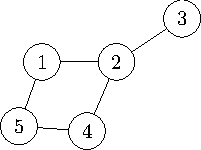
\includegraphics[width=0.4\textwidth]{chapters/gcol/figs/examplegraph1-figure2.pdf}
    \caption{Example undirected graph with at least one possible three-colouring solution (in fact, this graph is also potentially 2-colourable, and our \gls{cps} solution might select such a solution).}
    \label{fig:gcol:examplegraph}
\end{figure}

\begin{figure}
    \centering
    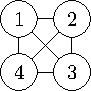
\includegraphics[width=0.2\textwidth]{chapters/gcol/figs/examplegraph1-figure3.pdf}
    \caption{Example undirected graph with no valid 3-colouring solutions.}
    \label{fig:gcol:examplegraphnosol}
\end{figure}

\subsection{Successful example}
For the graph in \autoref{fig:gcol:examplegraph}, we begin with a single top-level cell situated in the environment and in state \(s_0\).  From the hypothetical set of nodes \(V = \{1, 2, 3, 4, 5\}\) we derive the functor \(V' = \cpfunc{v}{\cpfunc{n}{1}~\cpfunc{n}{2}~\cpfunc{n}{3}~\cpfunc{n}{4}~\cpfunc{n}{5}}\), and the set of objects \[ 
E' = \{\cpfunc{e}{\cpfunc{n}{1} \, \cpfunc{n}{2}},~\cpfunc{e}{\cpfunc{n}{1} \, \cpfunc{n}{5}},~\cpfunc{e}{\cpfunc{n}{2} \, \cpfunc{n}{3}},~\cpfunc{e}{\cpfunc{n}{2} \, \cpfunc{n}{4}},~\cpfunc{e}{\cpfunc{n}{4} \, \cpfunc{n}{5}}\}
,\] representing the edges of the graph, as well as the set of colour objects \(K' = \{\cpfunc{k}{r},~\cpfunc{k}{g},~\cpfunc{k}{b}\}\), in this case representing the colours red, green and blue.  These sets of objects are all immediately within the top-level cell, along with \(\cpfunc{s}{1}\) to select node 1 at the beginning of the process, as shown in \autoref{objs:gcol:obj1}.

This beginning state, with the exception of the choice of node label inside the \(s\) object, is mandatory, but all following discussion in this subsection is merely one possible execution, due to the non-deterministic selection of colours that occurs during application of rule 1 and rule 2.

% \begin{figure}
% \begin{framed}
% \[
% e(\cpfunc{n}{1}\,\cpfunc{n}{2}) \quad \cpfunc{e}{\cpfunc{n}{1}\,\cpfunc{n}{5}} \quad \cpfunc{e}{\cpfunc{n}{2}\,\cpfunc{n}{3}} \quad \cpfunc{e}{\cpfunc{n}{2}\,\cpfunc{n}{4}} \quad \cpfunc{e}{\cpfunc{n}{4}\,\cpfunc{n}{5}}
% \]
% \[
% \cpfunc{k}{r} \quad \cpfunc{k}{g} \quad \cpfunc{k}{b} \quad \cpfunc{s}{1}\\
% \]
% \[
% \cpfunc{v}{\cpfunc{n}{1}~\cpfunc{n}{2}~\cpfunc{n}{3}~\cpfunc{n}{4}~\cpfunc{n}{5}}
% \]
% \end{framed}
% \caption{\label{fig:gcol:obj1}Initial set of objects inside the top-level cell for \autoref{fig:gcol:examplegraph}.}
% \end{figure}

\begin{cpobjectsfloat}
\begin{cpobjects}
\cpobjectsline{\cpfunc{e}{\cpfunc{n}{1} \, \cpfunc{n}{2}} \; \cpfunc{e}{\cpfunc{n}{1} \, \cpfunc{n}{5}} \; \cpfunc{e}{\cpfunc{n}{2} \, \cpfunc{n}{3}} \; \cpfunc{e}{\cpfunc{n}{2} \, \cpfunc{n}{4}} \; \cpfunc{e}{\cpfunc{n}{4} \, \cpfunc{n}{5}} \;}
% \[
% \cpfunc{e}{\cpfunc{n}{1}\,\cpfunc{n}{2}} \quad \cpfunc{e}{\cpfunc{n}{1}\,\cpfunc{n}{5}} \quad \cpfunc{e}{\cpfunc{n}{2}\,\cpfunc{n}{3}} \quad \cpfunc{e}{\cpfunc{n}{2}\,\cpfunc{n}{4}} \quad \cpfunc{e}{\cpfunc{n}{4}\,\cpfunc{n}{5}}
% \]
\cpobjectsline{ \cpfunc{k}{r} \; \cpfunc{k}{g} \; \cpfunc{k}{b} \quad \cpfunc{s}{1} \quad \cpfunc{v}{\cpfunc{n}{1} \; \cpfunc{n}{2} \; \cpfunc{n}{3} \; \cpfunc{n}{4} \; \cpfunc{n}{5}}}
% \[
% \cpfunc{k}{r} \quad \cpfunc{k}{g} \quad \cpfunc{k}{b} \quad \cpfunc{s}{1}\\
% \]
% \[
% \cpfunc{v}{\cpfunc{n}{1}~\cpfunc{n}{2}~\cpfunc{n}{3}~\cpfunc{n}{4}~\cpfunc{n}{5}}
% \]
\end{cpobjects}
\caption{\label{objs:gcol:obj1}Initial set of objects inside the top-level cell for \autoref{fig:gcol:examplegraph}.}
\end{cpobjectsfloat}

From this starting state, rule 1 is applied, choosing node 1 to start the process with, and selecting red as its colouring.  This creates the standard \(b\) and \(l\) objects.  No other rules are applicable at this point, as the top-level cell started in state \(s_0\).  The application of this rule leaves the top-level cell in state \(s_1\).  Rule 1 will henceforth be inapplicable, as the rules provide no way to revert to state \(s_0\).

% At the next step, rule 2 is checked but found inapplicable, as at this point the \(v\) object inside the only \(b\) object will not be empty, instead containing \(\cpfunc{v}{\cpfunc{n}{2}~ \cpfunc{n}{3}~ \cpfunc{n}{4}~ \cpfunc{n}{5}}\).  Rule 3, conversely, is applicable and thus can generate further new \(b\) objects.  In this instance, two edges exist from node 1 to other nodes (2 and 5 specifically), meaning that both choices can apply, generating new \(b\) objects containing all legal  colourings.  Both nodes are chosen to connect to, but there are only two other possible colourings to choose here, as red is currently blocked due to it being selected for the first \(b\) object.  This leads to the creation of four new \(b\) objects \(b\big(\cpfunc{l}{2}~\cpfunc{m}{\cpfunc{n}{1}\,\cpfunc{c}{r}}\allowbreak ~\cpfunc{m}{\cpfunc{n}{2}\,\cpfunc{c}{g}}\allowbreak ~\cpfunc{v}{\cpfunc{n}{3}~ \cpfunc{n}{4}~ \cpfunc{n}{5}}\big)\), \(b\big(\cpfunc{l}{2}~\cpfunc{m}{\cpfunc{n}{1}\,\cpfunc{c}{r}}\allowbreak ~\cpfunc{m}{\cpfunc{n}{5}\,\cpfunc{c}{b}}\allowbreak ~\cpfunc{v}{\cpfunc{n}{2}~ \cpfunc{n}{3}~ \cpfunc{n}{4}}\big)\) etc.

At the next step, rule 2 is checked but found inapplicable, as at this point the \(v\) object inside the only \(b\) object will not be empty, instead containing \(\cpfunc{v}{\cpfunc{n}{2}~ \cpfunc{n}{3}~ \cpfunc{n}{4}~ \cpfunc{n}{5}}\).  Rule 3, conversely, is applicable and thus can generate further new \(b\) objects.  In this instance, two edges exist from node 1 to other nodes (2 and 5 specifically), meaning that both choices can apply, generating new \(b\) objects containing all legal  colourings.  Both nodes are chosen to connect to, but there are only two other possible colourings to choose here, as red is currently blocked due to it being selected for the first \(b\) object.  This leads to the creation of four new \(b\) objects \(\cpfunc{b}{\cpfunc{l}{2}~\cpfunc{m}{\cpfunc{n}{1} \, \cpfunc{c}{r}}\allowbreak ~\cpfunc{m}{\cpfunc{n}{2} \, \cpfunc{c}{g}}\allowbreak ~\cpfunc{v}{\cpfunc{n}{3}~ \cpfunc{n}{4}~ \cpfunc{n}{5}}}\), \(\cpfunc{b}{\cpfunc{l}{2}~\cpfunc{m}{\cpfunc{n}{1} \, \cpfunc{c}{r}}\allowbreak ~\cpfunc{m}{\cpfunc{n}{5} \, \cpfunc{c}{b}}\allowbreak ~\cpfunc{v}{\cpfunc{n}{2}~ \cpfunc{n}{3}~ \cpfunc{n}{4}}}\) etc.

Simultaneously, rule 4 is applied to sweep away the pre-existing initial \(b\) object.  Rule 5 is not applicable because a state transition to state \(s_1\) has already been selected by application of rules 3 and 4, and thus a transition to state \(s_3\) is invalid.  Finally, rule 6 is also applied to remove the old \(l\) object and introduce a newly incremented one.  \autoref{objs:gcol:obj2} lists the objects in the top-level cell at the end of this step.

% \begin{figure}
% \begin{framed}
% \[
% e(\cpfunc{n}{1}\,\cpfunc{n}{2}) \quad \cpfunc{e}{\cpfunc{n}{1}\,\cpfunc{n}{5}} \quad \cpfunc{e}{\cpfunc{n}{2}\,\cpfunc{n}{3}} \quad \cpfunc{e}{\cpfunc{n}{2}\,\cpfunc{n}{4}} \quad \cpfunc{e}{\cpfunc{n}{4}\,\cpfunc{n}{5}}
% \]
% \[
%     \cpfunc{k}{r} \quad \cpfunc{k}{g} \quad \cpfunc{k}{b} \quad \cpfunc{l}{2}
% \]
% \[
% \cpfunc{b}{\cpfunc{l}{2}~\cpfunc{m}{\cpfunc{n}{1}\,\cpfunc{c}{r}}~\cpfunc{m}{\cpfunc{n}{2}\,\cpfunc{c}{g}}~\cpfunc{v}{\cpfunc{n}{3}~ \cpfunc{n}{4}~ \cpfunc{n}{5}}}
% \]
% \[
% \cpfunc{b}{\cpfunc{l}{2}~\cpfunc{m}{\cpfunc{n}{1}\,\cpfunc{c}{r}}~\cpfunc{m}{\cpfunc{n}{2}\,\cpfunc{c}{b}}~\cpfunc{v}{\cpfunc{n}{3}~ \cpfunc{n}{4}~ \cpfunc{n}{5}}}
% \]
% \[
% \cpfunc{b}{\cpfunc{l}{2}~\cpfunc{m}{\cpfunc{n}{1}\,\cpfunc{c}{r}}~\cpfunc{m}{\cpfunc{n}{5}\,\cpfunc{c}{g}}~\cpfunc{v}{\cpfunc{n}{2}~ \cpfunc{n}{3}~ \cpfunc{n}{4}}}
% \]
% \[
% \cpfunc{b}{\cpfunc{l}{2}~\cpfunc{m}{\cpfunc{n}{1}\,\cpfunc{c}{r}}~\cpfunc{m}{\cpfunc{n}{5}\,\cpfunc{c}{b}}~\cpfunc{v}{\cpfunc{n}{2}~ \cpfunc{n}{3}~ \cpfunc{n}{4}}}
% \]
% \end{framed}
% \caption{\label{fig:gcol:obj2}Set of objects inside the top-level cell after the second step (i.e. after one application of rules 3, 4 \& 6) for \autoref{fig:gcol:examplegraph}.}
% \end{figure}

\begin{cpobjectsfloat}
\begin{cpobjects}
\cpobjectsline{
\cpfunc{e}{\cpfunc{n}{1} \, \cpfunc{n}{2}} \; \cpfunc{e}{\cpfunc{n}{1} \, \cpfunc{n}{5}} \; \cpfunc{e}{\cpfunc{n}{2} \, \cpfunc{n}{3}} \; \cpfunc{e}{\cpfunc{n}{2} \, \cpfunc{n}{4}} \; \cpfunc{e}{\cpfunc{n}{4} \, \cpfunc{n}{5}}
}
\cpobjectsline{
    \cpfunc{k}{r} \; \cpfunc{k}{g} \; \cpfunc{k}{b} \quad \cpfunc{l}{2}
}
\cpobjectsline{
\cpfunc{b}{\cpfunc{l}{2}~\cpfunc{m}{\cpfunc{n}{1} \, \cpfunc{c}{r}}~\cpfunc{m}{\cpfunc{n}{2} \, \cpfunc{c}{g}}~\cpfunc{v}{\cpfunc{n}{3}~ \cpfunc{n}{4}~ \cpfunc{n}{5}}}
}
\cpobjectsline{
\cpfunc{b}{\cpfunc{l}{2}~\cpfunc{m}{\cpfunc{n}{1} \, \cpfunc{c}{r}}~\cpfunc{m}{\cpfunc{n}{2} \, \cpfunc{c}{b}}~\cpfunc{v}{\cpfunc{n}{3}~ \cpfunc{n}{4}~ \cpfunc{n}{5}}}
}
\cpobjectsline{
\cpfunc{b}{\cpfunc{l}{2}~\cpfunc{m}{\cpfunc{n}{1} \, \cpfunc{c}{r}}~\cpfunc{m}{\cpfunc{n}{5} \, \cpfunc{c}{g}}~\cpfunc{v}{\cpfunc{n}{2}~ \cpfunc{n}{3}~ \cpfunc{n}{4}}}
}
\cpobjectsline{
\cpfunc{b}{\cpfunc{l}{2}~\cpfunc{m}{\cpfunc{n}{1} \, \cpfunc{c}{r}}~\cpfunc{m}{\cpfunc{n}{5} \, \cpfunc{c}{b}}~\cpfunc{v}{\cpfunc{n}{2}~ \cpfunc{n}{3}~ \cpfunc{n}{4}}}
}
\end{cpobjects}
\caption{\label{objs:gcol:obj2}Set of objects inside the top-level cell after the second step (i.e. after one application of rules 3, 4 \& 6) for \autoref{fig:gcol:examplegraph}.}
\end{cpobjectsfloat}

The next step proceeds almost identically to the previous one, except that there are a greater number of new objects created (see \autoref{objs:gcol:obj3}).  At the previous step, the edges both between node 1 and node 5, and node 1 and node 2, were explored.  In this next step, edges between node 1 and node 5, node 1 and node 2 (where these edges were not explored previously for a given \(b\) object), node 5 and node 4, and node 2 and node 3 are all explored, with all objects that will not have direct colour conflicts instantiated as per rule 3.

% \begin{figure}
% \begin{framed}
% \begin{gather*}
%     \cpfunc{e}{\cpfunc{n}{1}\,\cpfunc{n}{2}} \quad \cpfunc{e}{\cpfunc{n}{1}\,\cpfunc{n}{5}} \quad \cpfunc{e}{\cpfunc{n}{2}\,\cpfunc{n}{3}} \quad \cpfunc{e}{\cpfunc{n}{2}\,\cpfunc{n}{4}} \quad \cpfunc{e}{\cpfunc{n}{4}\,\cpfunc{n}{5}}\\
%     \cpfunc{k}{r} \quad \cpfunc{k}{g} \quad \cpfunc{k}{b} \quad \cpfunc{l}{3}\\
%     \cpfunc{b}{\cpfunc{l}{3}~\cpfunc{m}{\cpfunc{n}{1}\,\cpfunc{c}{r}}~\cpfunc{m}{\cpfunc{n}{2}\,\cpfunc{c}{g}}~\cpfunc{m}{\cpfunc{n}{5}\,\cpfunc{c}{g}}~\cpfunc{v}{\cpfunc{n}{3}~ \cpfunc{n}{4}}} \\
%     \cpfunc{b}{\cpfunc{l}{3}~\cpfunc{m}{\cpfunc{n}{1}\,\cpfunc{c}{r}}~\cpfunc{m}{\cpfunc{n}{2}\,\cpfunc{c}{g}}~\cpfunc{m}{\cpfunc{n}{5}\,\cpfunc{c}{b}}~\cpfunc{v}{\cpfunc{n}{3}~ \cpfunc{n}{4}}} \\
%     \cpfunc{b}{\cpfunc{l}{3}~\cpfunc{m}{\cpfunc{n}{1}\,\cpfunc{c}{r}}~\cpfunc{m}{\cpfunc{n}{5}\,\cpfunc{c}{g}}~\cpfunc{m}{\cpfunc{n}{2}\,\cpfunc{c}{g}}~\cpfunc{v}{\cpfunc{n}{3}~ \cpfunc{n}{4}}} \\
%     \cpfunc{b}{\cpfunc{l}{3}~\cpfunc{m}{\cpfunc{n}{1}\,\cpfunc{c}{r}}~\cpfunc{m}{\cpfunc{n}{5}\,\cpfunc{c}{g}}~\cpfunc{m}{\cpfunc{n}{2}\,\cpfunc{c}{b}}~\cpfunc{v}{\cpfunc{n}{3}~ \cpfunc{n}{4}}} \\
%     \vdots\\
%     \cpfunc{b}{\cpfunc{l}{3}~\cpfunc{m}{\cpfunc{n}{1}\,\cpfunc{c}{r}}~\cpfunc{m}{\cpfunc{n}{2}\,\cpfunc{c}{b}}~\cpfunc{m}{\cpfunc{n}{3}\,\cpfunc{c}{r}}~\cpfunc{v}{\cpfunc{n}{4}~ \cpfunc{n}{5}}} \\
%     \cpfunc{b}{\cpfunc{l}{3}~\cpfunc{m}{\cpfunc{n}{1}\,\cpfunc{c}{r}}~\cpfunc{m}{\cpfunc{n}{2}\,\cpfunc{c}{b}}~\cpfunc{m}{\cpfunc{n}{3}\,\cpfunc{c}{g}}~\cpfunc{v}{\cpfunc{n}{4}~ \cpfunc{n}{5}}}
% \end{gather*}
% \end{framed}
% \caption{\label{fig:gcol:obj3}Set of objects inside the top-level cell after the third step for \autoref{fig:gcol:examplegraph}.  Note that there are some identical objects here which have been created independently.}
% \end{figure}

\begin{cpobjectsfloat}
\begin{cpobjects}
\begin{gather*}
    \cpfunc{e}{\cpfunc{n}{1} \, \cpfunc{n}{2}} \; \cpfunc{e}{\cpfunc{n}{1} \, \cpfunc{n}{5}} \; \cpfunc{e}{\cpfunc{n}{2} \, \cpfunc{n}{3}} \; \cpfunc{e}{\cpfunc{n}{2} \, \cpfunc{n}{4}} \; \cpfunc{e}{\cpfunc{n}{4} \, \cpfunc{n}{5}}\\
    \cpfunc{k}{r} \; \cpfunc{k}{g} \; \cpfunc{k}{b} \quad \cpfunc{l}{3}\\
    \cpfunc{b}{\cpfunc{l}{3}~\cpfunc{m}{\cpfunc{n}{1} \, \cpfunc{c}{r}}~\cpfunc{m}{\cpfunc{n}{2} \, \cpfunc{c}{g}}~\cpfunc{m}{\cpfunc{n}{5} \, \cpfunc{c}{g}}~\cpfunc{v}{\cpfunc{n}{3}~ \cpfunc{n}{4}}} \\
    \cpfunc{b}{\cpfunc{l}{3}~\cpfunc{m}{\cpfunc{n}{1} \, \cpfunc{c}{r}}~\cpfunc{m}{\cpfunc{n}{2} \, \cpfunc{c}{g}}~\cpfunc{m}{\cpfunc{n}{5} \, \cpfunc{c}{b}}~\cpfunc{v}{\cpfunc{n}{3}~ \cpfunc{n}{4}}} \\
    \cpfunc{b}{\cpfunc{l}{3}~\cpfunc{m}{\cpfunc{n}{1} \, \cpfunc{c}{r}}~\cpfunc{m}{\cpfunc{n}{5} \, \cpfunc{c}{g}}~\cpfunc{m}{\cpfunc{n}{2} \, \cpfunc{c}{g}}~\cpfunc{v}{\cpfunc{n}{3}~ \cpfunc{n}{4}}} \\
    \cpfunc{b}{\cpfunc{l}{3}~\cpfunc{m}{\cpfunc{n}{1} \, \cpfunc{c}{r}}~\cpfunc{m}{\cpfunc{n}{5} \, \cpfunc{c}{g}}~\cpfunc{m}{\cpfunc{n}{2} \, \cpfunc{c}{b}}~\cpfunc{v}{\cpfunc{n}{3}~ \cpfunc{n}{4}}} \\
    \vdots\\
    \cpfunc{b}{\cpfunc{l}{3}~\cpfunc{m}{\cpfunc{n}{1} \, \cpfunc{c}{r}}~\cpfunc{m}{\cpfunc{n}{2} \, \cpfunc{c}{b}}~\cpfunc{m}{\cpfunc{n}{3} \, \cpfunc{c}{r}}~\cpfunc{v}{\cpfunc{n}{4}~ \cpfunc{n}{5}}} \\
    \cpfunc{b}{\cpfunc{l}{3}~\cpfunc{m}{\cpfunc{n}{1} \, \cpfunc{c}{r}}~\cpfunc{m}{\cpfunc{n}{2} \, \cpfunc{c}{b}}~\cpfunc{m}{\cpfunc{n}{3} \, \cpfunc{c}{g}}~\cpfunc{v}{\cpfunc{n}{4}~ \cpfunc{n}{5}}}
\end{gather*}
\end{cpobjects}
\caption{\label{objs:gcol:obj3}Set of objects inside the top-level cell after the third step for \autoref{fig:gcol:examplegraph}.  Note that there are some identical objects here which have been created independently.}
\end{cpobjectsfloat}

At the fourth step, a large number of further objects are created, some of which are listed in \autoref{objs:gcol:obj4}.  The key difference between this step and the previous one is that the final inhibitor on rule 3 plays a much greater part.  At this step, many of the potential instantiations of new node and colouration selections will include conflicts between the newly-selected node and colour, and one or more of the node and colour selections made earlier.  The final inhibitor prevents instantiation of these choices, avoiding threats to correctness.  An alternative solution to the problem would be to include another following step, where those invalid instatiations are detected and removed, but the inhibitor makes this unnecessary.  

% \begin{figure}
% \begin{framed}
% \begin{gather*}
%     \cpfunc{e}{\cpfunc{n}{1}\,\cpfunc{n}{2}} \quad \cpfunc{e}{\cpfunc{n}{1}\,\cpfunc{n}{5}} \quad \cpfunc{e}{\cpfunc{n}{2}\,\cpfunc{n}{3}} \quad \cpfunc{e}{\cpfunc{n}{2}\,\cpfunc{n}{4}} \quad \cpfunc{e}{\cpfunc{n}{4}\,\cpfunc{n}{5}}\\
%     \cpfunc{k}{r} \quad \cpfunc{k}{g} \quad \cpfunc{k}{b} \quad \cpfunc{l}{4}\\
%     % \cpfunc{b}{\cpfunc{l}{3}~m(\cpfunc{n}{1}\,\cpfunc{c}{r}}~\cpfunc{m}{\cpfunc{n}{5}\,\cpfunc{c}{g}}~\cpfunc{m}{\cpfunc{n}{4}\,\cpfunc{c}{r}}~\cpfunc{v}{2~ 3}) \\
%     \cpfunc{b}{\cpfunc{l}{4}~\cpfunc{m}{\cpfunc{n}{1}\,\cpfunc{c}{r}}~\cpfunc{m}{\cpfunc{n}{5}\,\cpfunc{c}{g}}~\cpfunc{m}{\cpfunc{n}{4}\,\cpfunc{c}{r}}~\cpfunc{m}{\cpfunc{n}{2}\,\cpfunc{c}{g}}~\cpfunc{v}{\cpfunc{n}{3}}} \\
%     \cpfunc{b}{\cpfunc{l}{4}~\cpfunc{m}{\cpfunc{n}{1}\,\cpfunc{c}{r}}~\cpfunc{m}{\cpfunc{n}{5}\,\cpfunc{c}{g}}~\cpfunc{m}{\cpfunc{n}{4}\,\cpfunc{c}{r}}~\cpfunc{m}{\cpfunc{n}{2}\,\cpfunc{c}{b}}~\cpfunc{v}{\cpfunc{n}{3}}} \\
%     \cpfunc{b}{\cpfunc{l}{4}~\cpfunc{m}{\cpfunc{n}{1}\,\cpfunc{c}{r}}~\cpfunc{m}{\cpfunc{n}{5}\,\cpfunc{c}{g}}~\cpfunc{m}{\cpfunc{n}{4}\,\cpfunc{c}{r}}~\cpfunc{m}{\cpfunc{n}{2}\,\cpfunc{c}{g}}~\cpfunc{v}{\cpfunc{n}{3}}} \\
%     \cpfunc{b}{\cpfunc{l}{4}~\cpfunc{m}{\cpfunc{n}{1}\,\cpfunc{c}{r}}~\cpfunc{m}{\cpfunc{n}{5}\,\cpfunc{c}{g}}~\cpfunc{m}{\cpfunc{n}{4}\,\cpfunc{c}{r}}~\cpfunc{m}{\cpfunc{n}{2}\,\cpfunc{c}{b}}~\cpfunc{v}{\cpfunc{n}{3}}} \\
%     \vdots\\
%         \cpfunc{b}{\cpfunc{l}{4}~\cpfunc{m}{\cpfunc{n}{1}\,\cpfunc{c}{r}}~\cpfunc{m}{\cpfunc{n}{2}\,\cpfunc{c}{b}}~\cpfunc{m}{\cpfunc{n}{3}\,\cpfunc{c}{g}}~\cpfunc{m}{\cpfunc{n}{5}\,\cpfunc{c}{g}}~\cpfunc{v}{\cpfunc{n}{4}}} \\
%     \cpfunc{b}{\cpfunc{l}{4}~\cpfunc{m}{\cpfunc{n}{1}\,\cpfunc{c}{r}}~\cpfunc{m}{\cpfunc{n}{2}\,\cpfunc{c}{b}}~\cpfunc{m}{\cpfunc{n}{3}\,\cpfunc{c}{g}}~\cpfunc{m}{\cpfunc{n}{5}\,\cpfunc{c}{b}}~\cpfunc{v}{\cpfunc{n}{4}}}
% \end{gather*}
% \end{framed}
% \caption{\label{fig:gcol:obj4}Set of objects inside the top-level cell after the fourth step for \autoref{fig:gcol:examplegraph}.}
% \end{figure}  

\begin{cpobjectsfloat}
\begin{cpobjects}
\begin{gather*}
    \cpfunc{e}{\cpfunc{n}{1} \, \cpfunc{n}{2}} \; \cpfunc{e}{\cpfunc{n}{1} \, \cpfunc{n}{5}} \; \cpfunc{e}{\cpfunc{n}{2} \, \cpfunc{n}{3}} \; \cpfunc{e}{\cpfunc{n}{2} \, \cpfunc{n}{4}} \; \cpfunc{e}{\cpfunc{n}{4} \, \cpfunc{n}{5}}\\
    \cpfunc{k}{r} \; \cpfunc{k}{g} \; \cpfunc{k}{b} \quad \cpfunc{l}{4}\\
    % \cpfunc{b}{\cpfunc{l}{3}~m(\cpfunc{n}{1}\,\cpfunc{c}{r}}~\cpfunc{m}{\cpfunc{n}{5}\,\cpfunc{c}{g}}~\cpfunc{m}{\cpfunc{n}{4}\,\cpfunc{c}{r}}~\cpfunc{v}{2~ 3}) \\
    \cpfunc{b}{\cpfunc{l}{4}~\cpfunc{m}{\cpfunc{n}{1} \, \cpfunc{c}{r}}~\cpfunc{m}{\cpfunc{n}{5} \, \cpfunc{c}{g}}~\cpfunc{m}{\cpfunc{n}{4} \, \cpfunc{c}{r}}~\cpfunc{m}{\cpfunc{n}{2} \, \cpfunc{c}{g}}~\cpfunc{v}{\cpfunc{n}{3}}} \\
    \cpfunc{b}{\cpfunc{l}{4}~\cpfunc{m}{\cpfunc{n}{1} \, \cpfunc{c}{r}}~\cpfunc{m}{\cpfunc{n}{5} \, \cpfunc{c}{g}}~\cpfunc{m}{\cpfunc{n}{4} \, \cpfunc{c}{r}}~\cpfunc{m}{\cpfunc{n}{2} \, \cpfunc{c}{b}}~\cpfunc{v}{\cpfunc{n}{3}}} \\
    \cpfunc{b}{\cpfunc{l}{4}~\cpfunc{m}{\cpfunc{n}{1} \, \cpfunc{c}{r}}~\cpfunc{m}{\cpfunc{n}{5} \, \cpfunc{c}{g}}~\cpfunc{m}{\cpfunc{n}{4} \, \cpfunc{c}{r}}~\cpfunc{m}{\cpfunc{n}{2} \, \cpfunc{c}{g}}~\cpfunc{v}{\cpfunc{n}{3}}} \\
    \cpfunc{b}{\cpfunc{l}{4}~\cpfunc{m}{\cpfunc{n}{1} \, \cpfunc{c}{r}}~\cpfunc{m}{\cpfunc{n}{5} \, \cpfunc{c}{g}}~\cpfunc{m}{\cpfunc{n}{4} \, \cpfunc{c}{r}}~\cpfunc{m}{\cpfunc{n}{2} \, \cpfunc{c}{b}}~\cpfunc{v}{\cpfunc{n}{3}}} \\
    \vdots\\
        \cpfunc{b}{\cpfunc{l}{4}~\cpfunc{m}{\cpfunc{n}{1} \, \cpfunc{c}{r}}~\cpfunc{m}{\cpfunc{n}{2} \, \cpfunc{c}{b}}~\cpfunc{m}{\cpfunc{n}{3} \, \cpfunc{c}{g}}~\cpfunc{m}{\cpfunc{n}{5} \, \cpfunc{c}{g}}~\cpfunc{v}{\cpfunc{n}{4}}} \\
    \cpfunc{b}{\cpfunc{l}{4}~\cpfunc{m}{\cpfunc{n}{1} \, \cpfunc{c}{r}}~\cpfunc{m}{\cpfunc{n}{2} \, \cpfunc{c}{b}}~\cpfunc{m}{\cpfunc{n}{3} \, \cpfunc{c}{g}}~\cpfunc{m}{\cpfunc{n}{5} \, \cpfunc{c}{b}}~\cpfunc{v}{\cpfunc{n}{4}}}
\end{gather*}

\end{cpobjects}
\caption{\label{objs:gcol:obj4}Set of objects inside the top-level cell after the fourth step for \autoref{fig:gcol:examplegraph}.}
\end{cpobjectsfloat}

Step 5 proceeds analogously.  At the end of step 5 a number of \(b\) objects which contain valid colourings of the whole graph will be present inside the top-level cell.  At the sixth step, rule 2 will detect this by the fact that said objects will contain empty \(v\) functors.  For example, \autoref{objs:gcol:obj6} shows some of the potential solutions that could be generated, reflecting the state of the system at the end of the fifth step.  In fact, the first potential solution shows that in this case it is possible to completely and validly colour this graph using only two colours.  This solution may or may not be chosen when rule 2 is applied.  At the end of the sixth step, rule 2 will select one of the possible solutions and emit it to the environment.  The top-level cell will also transition to state \(s_2\), signalling that the process succeeded.

% \begin{figure}
% \begin{framed}
% \begin{gather*}
%     \cpfunc{e}{\cpfunc{n}{1}\,\cpfunc{n}{2}} \quad \cpfunc{e}{\cpfunc{n}{1}\,\cpfunc{n}{5}} \quad \cpfunc{e}{\cpfunc{n}{2}\,\cpfunc{n}{3}} \quad \cpfunc{e}{\cpfunc{n}{2}\,\cpfunc{n}{4}} \quad \cpfunc{e}{\cpfunc{n}{4}\,\cpfunc{n}{5}}\\
%     \cpfunc{k}{r} \quad \cpfunc{k}{g} \quad \cpfunc{k}{b} \quad \cpfunc{l}{5}\\
%     \cpfunc{b}{\cpfunc{l}{5}~\cpfunc{m}{\cpfunc{n}{1}\,\cpfunc{c}{r}}~\cpfunc{m}{\cpfunc{n}{5}\,\cpfunc{c}{g}}~\cpfunc{m}{\cpfunc{n}{4}\,\cpfunc{c}{r}}~\cpfunc{m}{\cpfunc{n}{2}\,\cpfunc{c}{g}}~\cpfunc{m}{\cpfunc{n}{3}\,\cpfunc{c}{r}}~v()} \\
%     \cpfunc{b}{\cpfunc{l}{5}~\cpfunc{m}{\cpfunc{n}{1}\,\cpfunc{c}{r}}~\cpfunc{m}{\cpfunc{n}{5}\,\cpfunc{c}{g}}~\cpfunc{m}{\cpfunc{n}{4}\,\cpfunc{c}{r}}~\cpfunc{m}{\cpfunc{n}{2}\,\cpfunc{c}{g}}~\cpfunc{m}{\cpfunc{n}{3}\,\cpfunc{c}{b}}~v()} \\
%             \vdots\\
%     \cpfunc{b}{\cpfunc{l}{5}~\cpfunc{m}{\cpfunc{n}{1}\,\cpfunc{c}{r}}~\cpfunc{m}{\cpfunc{n}{2}\,\cpfunc{c}{b}}~\cpfunc{m}{\cpfunc{n}{3}\,\cpfunc{c}{g}}~\cpfunc{m}{\cpfunc{n}{5}\,\cpfunc{c}{g}}~\cpfunc{m}{\cpfunc{n}{4}\,\cpfunc{c}{r}}~v()} \\
%     \cpfunc{b}{\cpfunc{l}{5}~\cpfunc{m}{\cpfunc{n}{1}\,\cpfunc{c}{r}}~\cpfunc{m}{\cpfunc{n}{2}\,\cpfunc{c}{b}}~\cpfunc{m}{\cpfunc{n}{3}\,\cpfunc{c}{g}}~\cpfunc{m}{\cpfunc{n}{5}\,\cpfunc{c}{g}}~\cpfunc{m}{\cpfunc{n}{4}\,\cpfunc{c}{r}}~v()}
% \end{gather*}
% \end{framed}
% \caption{\label{fig:obj6}Set of objects inside the top-level cell after the fifth step for \autoref{fig:gcol:examplegraph}.}
% \end{figure}

\begin{cpobjectsfloat}
\begin{cpobjects}

\begin{gather*}
    \cpfunc{e}{\cpfunc{n}{1} \, \cpfunc{n}{2}} \; \cpfunc{e}{\cpfunc{n}{1} \, \cpfunc{n}{5}} \; \cpfunc{e}{\cpfunc{n}{2} \, \cpfunc{n}{3}} \; \cpfunc{e}{\cpfunc{n}{2} \, \cpfunc{n}{4}} \; \cpfunc{e}{\cpfunc{n}{4} \, \cpfunc{n}{5}}\\
    \cpfunc{k}{r} \; \cpfunc{k}{g} \; \cpfunc{k}{b} \quad \cpfunc{l}{5}\\
    \cpfunc{b}{\cpfunc{l}{5}~\cpfunc{m}{\cpfunc{n}{1} \, \cpfunc{c}{r}}~\cpfunc{m}{\cpfunc{n}{5} \, \cpfunc{c}{g}}~\cpfunc{m}{\cpfunc{n}{4} \, \cpfunc{c}{r}}~\cpfunc{m}{\cpfunc{n}{2} \, \cpfunc{c}{g}}~\cpfunc{m}{\cpfunc{n}{3} \, \cpfunc{c}{r}}~v()} \\
    \cpfunc{b}{\cpfunc{l}{5}~\cpfunc{m}{\cpfunc{n}{1} \, \cpfunc{c}{r}}~\cpfunc{m}{\cpfunc{n}{5} \, \cpfunc{c}{g}}~\cpfunc{m}{\cpfunc{n}{4} \, \cpfunc{c}{r}}~\cpfunc{m}{\cpfunc{n}{2} \, \cpfunc{c}{g}}~\cpfunc{m}{\cpfunc{n}{3} \, \cpfunc{c}{b}}~v()} \\
            \vdots\\
    \cpfunc{b}{\cpfunc{l}{5}~\cpfunc{m}{\cpfunc{n}{1} \, \cpfunc{c}{r}}~\cpfunc{m}{\cpfunc{n}{2} \, \cpfunc{c}{b}}~\cpfunc{m}{\cpfunc{n}{3} \, \cpfunc{c}{g}}~\cpfunc{m}{\cpfunc{n}{5} \, \cpfunc{c}{g}}~\cpfunc{m}{\cpfunc{n}{4} \, \cpfunc{c}{r}}~v()} \\
    \cpfunc{b}{\cpfunc{l}{5}~\cpfunc{m}{\cpfunc{n}{1} \, \cpfunc{c}{r}}~\cpfunc{m}{\cpfunc{n}{2} \, \cpfunc{c}{b}}~\cpfunc{m}{\cpfunc{n}{3} \, \cpfunc{c}{g}}~\cpfunc{m}{\cpfunc{n}{5} \, \cpfunc{c}{g}}~\cpfunc{m}{\cpfunc{n}{4} \, \cpfunc{c}{r}}~v()}
\end{gather*}
\end{cpobjects}
\caption{\label{objs:gcol:obj6}Set of objects inside the top-level cell after the fifth step for \autoref{fig:gcol:examplegraph}.}
\end{cpobjectsfloat}

% ------------------------------------------------

\subsection{Failure example}
Here we step through the execution of the algorithm when there is no possible valid 3-colouring solution, using the graph depicted in \autoref{fig:gcol:examplegraphnosol}.  The system begins with the objects depicted in \autoref{objs:gcol:objn1}.

% \begin{figure}
% \begin{framed}
% \begin{gather*}
%     \cpfunc{e}{\cpfunc{n}{1}\,\cpfunc{n}{2}} \quad \cpfunc{e}{\cpfunc{n}{1}\,\cpfunc{n}{3}} \quad \cpfunc{e}{\cpfunc{n}{1}\,\cpfunc{n}{4}} \quad \cpfunc{e}{\cpfunc{n}{2}\,\cpfunc{n}{3}} \quad \cpfunc{e}{\cpfunc{n}{2}\,\cpfunc{n}{4}} \quad \cpfunc{e}{\cpfunc{n}{3}\,\cpfunc{n}{4}}\\
%     \cpfunc{k}{r} \quad \cpfunc{k}{g} \quad \cpfunc{k}{b} \quad \cpfunc{s}{1}\\
%     \cpfunc{v}{\cpfunc{n}{1}~\cpfunc{n}{2}~\cpfunc{n}{3}~\cpfunc{n}{4}}
% \end{gather*}
% \end{framed}
% \caption{\label{fig:objn1}Initial set of objects inside the top-level cell for \autoref{fig:gcol:examplegraphnosol}.}
% \end{figure}

\begin{cpobjectsfloat}
\begin{cpobjects}

\begin{gather*}
    \cpfunc{e}{\cpfunc{n}{1} \, \cpfunc{n}{2}} \; \cpfunc{e}{\cpfunc{n}{1} \, \cpfunc{n}{3}} \; \cpfunc{e}{\cpfunc{n}{1} \, \cpfunc{n}{4}} \; \cpfunc{e}{\cpfunc{n}{2} \, \cpfunc{n}{3}} \; \cpfunc{e}{\cpfunc{n}{2} \, \cpfunc{n}{4}} \; \cpfunc{e}{\cpfunc{n}{3} \, \cpfunc{n}{4}}\\
    \cpfunc{k}{r} \; \cpfunc{k}{g} \; \cpfunc{k}{b} \quad \cpfunc{s}{1}\\
    \cpfunc{v}{\cpfunc{n}{1}~\cpfunc{n}{2}~\cpfunc{n}{3}~\cpfunc{n}{4}}
\end{gather*}
\end{cpobjects}
\caption{\label{objs:gcol:objn1}Initial set of objects inside the top-level cell for \autoref{fig:gcol:examplegraphnosol}.}
\end{cpobjectsfloat}

After the first step, the application of rule 1, the objects shown in \autoref{objs:gcol:objn2} are inside the top-level cell.  This is not substantively different from the successful example above.  Likewise with the objects present in the cell at the end of the second step, shown in \autoref{objs:gcol:objn3}.

% \begin{figure}
% \begin{framed}
% \begin{gather*}
%     \cpfunc{e}{\cpfunc{n}{1}\,\cpfunc{n}{2}} \quad \cpfunc{e}{\cpfunc{n}{1}\,\cpfunc{n}{3}} \quad \cpfunc{e}{\cpfunc{n}{1}\,\cpfunc{n}{4}} \quad \cpfunc{e}{\cpfunc{n}{2}\,\cpfunc{n}{3}} \quad \cpfunc{e}{\cpfunc{n}{2}\,\cpfunc{n}{4}} \quad \cpfunc{e}{\cpfunc{n}{3}\,\cpfunc{n}{4}}\\
%     \cpfunc{k}{r} \quad \cpfunc{k}{g} \quad \cpfunc{k}{b} \quad \cpfunc{l}{1}\\
%     \cpfunc{b}{\cpfunc{l}{1}~\cpfunc{m}{\cpfunc{n}{1}\,\cpfunc{c}{r}}~\cpfunc{v}{\cpfunc{n}{2}~\cpfunc{n}{3}~\cpfunc{n}{4}}}
% \end{gather*}
% \end{framed}
% \caption{\label{fig:objn2}Set of objects inside the top-level cell at the end of step 1, for \autoref{fig:gcol:examplegraphnosol}.}
% \end{figure}

\begin{cpobjectsfloat}
\begin{cpobjects}

\begin{gather*}
    \cpfunc{e}{\cpfunc{n}{1} \, \cpfunc{n}{2}} \; \cpfunc{e}{\cpfunc{n}{1} \, \cpfunc{n}{3}} \; \cpfunc{e}{\cpfunc{n}{1} \, \cpfunc{n}{4}} \; \cpfunc{e}{\cpfunc{n}{2} \, \cpfunc{n}{3}} \; \cpfunc{e}{\cpfunc{n}{2} \, \cpfunc{n}{4}} \; \cpfunc{e}{\cpfunc{n}{3} \, \cpfunc{n}{4}}\\
    \cpfunc{k}{r} \; \cpfunc{k}{g} \; \cpfunc{k}{b} \quad \cpfunc{l}{1}\\
    \cpfunc{b}{\cpfunc{l}{1}~\cpfunc{m}{\cpfunc{n}{1} \, \cpfunc{c}{r}}~\cpfunc{v}{\cpfunc{n}{2}~\cpfunc{n}{3}~\cpfunc{n}{4}}}
\end{gather*}
\end{cpobjects}
\caption{\label{objs:gcol:objn2}Set of objects inside the top-level cell at the end of step 1, for \autoref{fig:gcol:examplegraphnosol}.}
\end{cpobjectsfloat}

% \begin{figure}
% \begin{framed}
% \begin{gather*}
%     \cpfunc{e}{\cpfunc{n}{1}\,\cpfunc{n}{2}} \quad \cpfunc{e}{\cpfunc{n}{1}\,\cpfunc{n}{3}} \quad \cpfunc{e}{\cpfunc{n}{1}\,\cpfunc{n}{4}} \quad \cpfunc{e}{\cpfunc{n}{2}\,\cpfunc{n}{3}} \quad \cpfunc{e}{\cpfunc{n}{2}\,\cpfunc{n}{4}} \quad \cpfunc{e}{\cpfunc{n}{3}\,\cpfunc{n}{4}}\\
%     \cpfunc{k}{r} \quad \cpfunc{k}{g} \quad \cpfunc{k}{b} \quad \cpfunc{l}{2}\\
%     \cpfunc{b}{\cpfunc{l}{2}~\cpfunc{m}{\cpfunc{n}{1}\,\cpfunc{c}{r}}~\cpfunc{m}{\cpfunc{n}{2}\,\cpfunc{c}{g}}~\cpfunc{v}{\cpfunc{n}{3}~\cpfunc{n}{4}}}\\
%     \cpfunc{b}{\cpfunc{l}{2}~\cpfunc{m}{\cpfunc{n}{1}\,\cpfunc{c}{r}}~\cpfunc{m}{\cpfunc{n}{2}\,\cpfunc{c}{b}}~\cpfunc{v}{\cpfunc{n}{3}~\cpfunc{n}{4}}}\\
%     \cpfunc{b}{\cpfunc{l}{2}~\cpfunc{m}{\cpfunc{n}{1}\,\cpfunc{c}{r}}~\cpfunc{m}{\cpfunc{n}{3}\,\cpfunc{c}{g}}~\cpfunc{v}{\cpfunc{n}{2}~\cpfunc{n}{4}}}\\
%     \cpfunc{b}{\cpfunc{l}{2}~\cpfunc{m}{\cpfunc{n}{1}\,\cpfunc{c}{r}}~\cpfunc{m}{\cpfunc{n}{3}\,\cpfunc{c}{b}}~\cpfunc{v}{\cpfunc{n}{2}~\cpfunc{n}{4}}}\\
%     \cpfunc{b}{\cpfunc{l}{2}~\cpfunc{m}{\cpfunc{n}{1}\,\cpfunc{c}{r}}~\cpfunc{m}{\cpfunc{n}{4}\,\cpfunc{c}{g}}~\cpfunc{v}{\cpfunc{n}{2}~\cpfunc{n}{3}}}\\
%     \cpfunc{b}{\cpfunc{l}{2}~\cpfunc{m}{\cpfunc{n}{1}\,\cpfunc{c}{r}}~\cpfunc{m}{\cpfunc{n}{4}\,\cpfunc{c}{b}}~\cpfunc{v}{\cpfunc{n}{2}~\cpfunc{n}{3}}}
% \end{gather*}
% \end{framed}
% \caption{\label{fig:objn3}Set of objects inside the top-level cell at the end of step 2, for \autoref{fig:gcol:examplegraphnosol}.}
% \end{figure}

\begin{cpobjectsfloat}
\begin{cpobjects}
\begin{gather*}
    \cpfunc{e}{\cpfunc{n}{1} \, \cpfunc{n}{2}} \; \cpfunc{e}{\cpfunc{n}{1} \, \cpfunc{n}{3}} \; \cpfunc{e}{\cpfunc{n}{1} \, \cpfunc{n}{4}} \; \cpfunc{e}{\cpfunc{n}{2} \, \cpfunc{n}{3}} \; \cpfunc{e}{\cpfunc{n}{2} \, \cpfunc{n}{4}} \; \cpfunc{e}{\cpfunc{n}{3} \, \cpfunc{n}{4}}\\
    \cpfunc{k}{r} \; \cpfunc{k}{g} \; \cpfunc{k}{b} \quad \cpfunc{l}{2}\\
    \cpfunc{b}{\cpfunc{l}{2}~\cpfunc{m}{\cpfunc{n}{1} \, \cpfunc{c}{r}}~\cpfunc{m}{\cpfunc{n}{2} \, \cpfunc{c}{g}}~\cpfunc{v}{\cpfunc{n}{3}~\cpfunc{n}{4}}}\\
    \cpfunc{b}{\cpfunc{l}{2}~\cpfunc{m}{\cpfunc{n}{1} \, \cpfunc{c}{r}}~\cpfunc{m}{\cpfunc{n}{2} \, \cpfunc{c}{b}}~\cpfunc{v}{\cpfunc{n}{3}~\cpfunc{n}{4}}}\\
    \cpfunc{b}{\cpfunc{l}{2}~\cpfunc{m}{\cpfunc{n}{1} \, \cpfunc{c}{r}}~\cpfunc{m}{\cpfunc{n}{3} \, \cpfunc{c}{g}}~\cpfunc{v}{\cpfunc{n}{2}~\cpfunc{n}{4}}}\\
    \cpfunc{b}{\cpfunc{l}{2}~\cpfunc{m}{\cpfunc{n}{1} \, \cpfunc{c}{r}}~\cpfunc{m}{\cpfunc{n}{3} \, \cpfunc{c}{b}}~\cpfunc{v}{\cpfunc{n}{2}~\cpfunc{n}{4}}}\\
    \cpfunc{b}{\cpfunc{l}{2}~\cpfunc{m}{\cpfunc{n}{1} \, \cpfunc{c}{r}}~\cpfunc{m}{\cpfunc{n}{4} \, \cpfunc{c}{g}}~\cpfunc{v}{\cpfunc{n}{2}~\cpfunc{n}{3}}}\\
    \cpfunc{b}{\cpfunc{l}{2}~\cpfunc{m}{\cpfunc{n}{1} \, \cpfunc{c}{r}}~\cpfunc{m}{\cpfunc{n}{4} \, \cpfunc{c}{b}}~\cpfunc{v}{\cpfunc{n}{2}~\cpfunc{n}{3}}}
\end{gather*}

\end{cpobjects}
\caption{\label{objs:gcol:objn3}Set of objects inside the top-level cell at the end of step 2, for \autoref{fig:gcol:examplegraphnosol}.}
\end{cpobjectsfloat}

\autoref{objs:gcol:objn4} shows the objects in the top-level cell at the end of step three.  This proceeds in much the same fashion as the previous step, but fully half of the potential instantiations from rule 3 are avoided by the rule's final inhibitor, due to inevitable colouration conflicts.

% \begin{figure}
% \begin{framed}
% \begin{gather*}
%     \cpfunc{e}{\cpfunc{n}{1}\,\cpfunc{n}{2}} \quad \cpfunc{e}{\cpfunc{n}{1}\,\cpfunc{n}{3}} \quad \cpfunc{e}{\cpfunc{n}{1}\,\cpfunc{n}{4}} \quad \cpfunc{e}{\cpfunc{n}{2}\,\cpfunc{n}{3}} \quad \cpfunc{e}{\cpfunc{n}{2}\,\cpfunc{n}{4}} \quad \cpfunc{e}{\cpfunc{n}{3}\,\cpfunc{n}{4}}\\
%     \cpfunc{k}{r} \quad \cpfunc{k}{g} \quad \cpfunc{k}{b} \quad \cpfunc{l}{3}\\
%     % \cpfunc{b}{\cpfunc{l}{2}~m(\cpfunc{n}{1}\,\cpfunc{c}{r}}~\cpfunc{m}{\cpfunc{n}{2}\,\cpfunc{c}{g}}~\cpfunc{v}{\cpfunc{n}{3}~\cpfunc{n}{4}})\\
%     \cpfunc{b}{\cpfunc{l}{3}~\cpfunc{m}{\cpfunc{n}{1}\,\cpfunc{c}{r}}~\cpfunc{m}{\cpfunc{n}{2}\,\cpfunc{c}{g}}~\cpfunc{m}{\cpfunc{n}{3}\,\cpfunc{c}{b}}~\cpfunc{v}{\cpfunc{n}{4}}}\\
%     \cpfunc{b}{\cpfunc{l}{3}~\cpfunc{m}{\cpfunc{n}{1}\,\cpfunc{c}{r}}~\cpfunc{m}{\cpfunc{n}{2}\,\cpfunc{c}{g}}~\cpfunc{m}{\cpfunc{n}{3}\,\cpfunc{c}{b}}~\cpfunc{v}{\cpfunc{n}{4}}}\\
%         \vdots\\
%     \cpfunc{b}{\cpfunc{l}{3}~\cpfunc{m}{\cpfunc{n}{1}\,\cpfunc{c}{r}}~\cpfunc{m}{\cpfunc{n}{2}\,\cpfunc{c}{g}}~\cpfunc{m}{\cpfunc{n}{4}\,\cpfunc{c}{b}}~\cpfunc{v}{\cpfunc{n}{3}}}\\
%     \cpfunc{b}{\cpfunc{l}{3}~\cpfunc{m}{\cpfunc{n}{1}\,\cpfunc{c}{r}}~\cpfunc{m}{\cpfunc{n}{2}\,\cpfunc{c}{g}}~\cpfunc{m}{\cpfunc{n}{4}\,\cpfunc{c}{b}}~\cpfunc{v}{\cpfunc{n}{3}}}
% \end{gather*}
% \end{framed}
% \caption{\label{fig:objn4}Set of objects inside the top-level cell at the end of step 3, for \autoref{fig:gcol:examplegraphnosol}.}
% \end{figure}

\begin{cpobjectsfloat}
\begin{cpobjects}

\begin{gather*}
    \cpfunc{e}{\cpfunc{n}{1} \, \cpfunc{n}{2}} \; \cpfunc{e}{\cpfunc{n}{1} \, \cpfunc{n}{3}} \; \cpfunc{e}{\cpfunc{n}{1} \, \cpfunc{n}{4}} \; \cpfunc{e}{\cpfunc{n}{2} \, \cpfunc{n}{3}} \; \cpfunc{e}{\cpfunc{n}{2} \, \cpfunc{n}{4}} \; \cpfunc{e}{\cpfunc{n}{3} \, \cpfunc{n}{4}}\\
    \cpfunc{k}{r} \; \cpfunc{k}{g} \; \cpfunc{k}{b} \quad \cpfunc{l}{3}\\
    % \cpfunc{b}{\cpfunc{l}{2}~m(\cpfunc{n}{1}\,\cpfunc{c}{r}}~\cpfunc{m}{\cpfunc{n}{2}\,\cpfunc{c}{g}}~\cpfunc{v}{\cpfunc{n}{3}~\cpfunc{n}{4}})\\
    \cpfunc{b}{\cpfunc{l}{3}~\cpfunc{m}{\cpfunc{n}{1} \, \cpfunc{c}{r}}~\cpfunc{m}{\cpfunc{n}{2} \, \cpfunc{c}{g}}~\cpfunc{m}{\cpfunc{n}{3} \, \cpfunc{c}{b}}~\cpfunc{v}{\cpfunc{n}{4}}}\\
    \cpfunc{b}{\cpfunc{l}{3}~\cpfunc{m}{\cpfunc{n}{1} \, \cpfunc{c}{r}}~\cpfunc{m}{\cpfunc{n}{2} \, \cpfunc{c}{g}}~\cpfunc{m}{\cpfunc{n}{3} \, \cpfunc{c}{b}}~\cpfunc{v}{\cpfunc{n}{4}}}\\
        \vdots\\
    \cpfunc{b}{\cpfunc{l}{3}~\cpfunc{m}{\cpfunc{n}{1} \, \cpfunc{c}{r}}~\cpfunc{m}{\cpfunc{n}{2} \, \cpfunc{c}{g}}~\cpfunc{m}{\cpfunc{n}{4} \, \cpfunc{c}{b}}~\cpfunc{v}{\cpfunc{n}{3}}}\\
    \cpfunc{b}{\cpfunc{l}{3}~\cpfunc{m}{\cpfunc{n}{1} \, \cpfunc{c}{r}}~\cpfunc{m}{\cpfunc{n}{2} \, \cpfunc{c}{g}}~\cpfunc{m}{\cpfunc{n}{4} \, \cpfunc{c}{b}}~\cpfunc{v}{\cpfunc{n}{3}}}
\end{gather*}
\end{cpobjects}
\caption{\label{objs:gcol:objn4}Set of objects inside the top-level cell at the end of step 3, for \autoref{fig:gcol:examplegraphnosol}.}
\end{cpobjectsfloat}

Finally, \autoref{objs:gcol:objn5} shows the objects in the top-level cell as at the end of step 4.  Due to the fully-connected nature of the graph in \autoref{fig:gcol:examplegraphnosol}, every possible solution will contain at least one instance of proposed contiguous colouration, thus making every possible solution invalid.  This means that rule 3 will not create any new \(b\) objects, while rule 4 will remove the pre-existing ones.

% \begin{figure}
% \begin{framed}
% \begin{gather*}
%     \cpfunc{e}{\cpfunc{n}{1}\,\cpfunc{n}{2}} \quad \cpfunc{e}{\cpfunc{n}{1}\,\cpfunc{n}{3}} \quad \cpfunc{e}{\cpfunc{n}{1}\,\cpfunc{n}{4}} \quad \cpfunc{e}{\cpfunc{n}{2}\,\cpfunc{n}{3}} \quad \cpfunc{e}{\cpfunc{n}{2}\,\cpfunc{n}{4}} \quad \cpfunc{e}{\cpfunc{n}{3}\,\cpfunc{n}{4}}\\
%     \cpfunc{k}{r} \quad \cpfunc{k}{g} \quad \cpfunc{k}{b} \quad \cpfunc{l}{4}
% \end{gather*}
% \end{framed}
% \caption{\label{fig:objn5}Set of objects inside the top-level cell at the end of step 4, for \autoref{fig:gcol:examplegraphnosol}.}
% \end{figure}

\begin{cpobjectsfloat}
\begin{cpobjects}

\begin{gather*}
    \cpfunc{e}{\cpfunc{n}{1} \, \cpfunc{n}{2}} \; \cpfunc{e}{\cpfunc{n}{1} \, \cpfunc{n}{3}} \; \cpfunc{e}{\cpfunc{n}{1} \, \cpfunc{n}{4}} \; \cpfunc{e}{\cpfunc{n}{2} \, \cpfunc{n}{3}} \; \cpfunc{e}{\cpfunc{n}{2} \, \cpfunc{n}{4}} \; \cpfunc{e}{\cpfunc{n}{3} \, \cpfunc{n}{4}}\\
    \cpfunc{k}{r} \; \cpfunc{k}{g} \; \cpfunc{k}{b} \quad \cpfunc{l}{4}
\end{gather*}
\end{cpobjects}
\caption{\label{objs:gcol:objn5}Set of objects inside the top-level cell at the end of step 4, for \autoref{fig:gcol:examplegraphnosol}.}
\end{cpobjectsfloat}

With no \(b\) objects available in the system, at the next step none of rules 1-4 will be applicable.  Thus, the first rule selected is rule 5, which merely transitions the top-level cell to state \(s_3\), signalling to the environment that the evolution of the system has ceased after determining that there was no possible valid colouring for the graph using the colours provided.

% \section{\label{sec:gcol:conc}Conclusions}
% Firstly we implemented a version of Gheorghe \textit{et al.}'s \gls{skps} solution to the 3-colouring problem using \fsharp{} and a \gls{cml}-derived library, Hopac.   On the small sample of graphs tested this produces reasonable results for smaller graphs, at least as good as those achieved by the P-Lingua/MeCoSim simulation.  In both systems, the inclusion of a test for already-invalid compartments has the potential to improve the runtimes significantly, as it prunes the search space, sometimes quite dramatically.

% \gls{cml} appears to be a good fit in principle to \gls{ps} variants that use communication between cells/membranes, but this particular problem had fairly minimal communication and instead relied heavily upon cell division.  Further testing with other problems is required to determine the efficacy of \gls{cml} for sure.

% We secondly provided a single-top-level-cell \gls{cps} solution to the Graph Colouring Problem, which is capable of solving the problem for arbitrary graphs with an arbitrary number of potential colours in at most \(|V| + 1\) steps.  Its operation was demonstrated with two 3-colouring examples based on two different graphs, for which it was and was not possible, respectively, to find a valid 3-colouring.

\citeauthor{Gheorghe2013} presented a \gls{ps} solution to the 3-colouring problem, using communicating \gls{skps} \cite{Gheorghe2013}.  Based on this work, we first discuss in \autoref{sec:gcol:cml} a \gls{cml} implementation of the \gls{skps} solution in \cite{Gheorghe2013}, briefly compare the two approaches and indicate some other \gls{ps} variants we think \gls{cml} might be a good fit with.  We then present in \autoref{sec:gcol:cpsys} a concise single-cell solution to the problem using \gls{cps}, and provide an informal analysis of it.  Lastly, in \autoref{sec:gcol:examples}, we provide examples of the operation of our cP~system on the 3-colour problem, both for a graph that is colourable and one that is not, before concluding in \autoref{sec:gcol:conc}.

So far as known, this is the first time \gls{cps} has been applied to graph colouring, and the first time that a \gls{cml} implementation has been used to simulate the operation of any P~system.

\section[Simple Kernel P Systems Solution to the \glsfmtname{gcp-glossary} in \glsfmtname{cml-glossary}][\Gls{skps} Solution to the \gls{gcp} in \gls{cml}]{\label{sec:gcol:cml}Simple Kernel P Systems Solution to the \glsfmtlong{gcp-glossary} in \glsfmtlong{cml-glossary}}

This \namecref{sec:gcol:cml} explores \gls{cml} as another methodology to use for simulating \gls{ps} where communication is involved.  For a first experiment, it implements \citeauthor{Gheorghe2013}'s 3-colouring problem solution from \cite{Gheorghe2013}, as it involves communication between \glspl{compartment} but is relatively low-complexity and thus appears to be suitable for a first attempt at simulating communicating \gls{ps} with \gls{cml}.

The programming language \fsharp{} was used with the library Hopac,\footnote{\url{https://github.com/Hopac/Hopac}} which is modelled on \gls{cml} and follows it closely.\footnote{The final program can be found at \url{https://github.com/jcoo092/acmc2018}}  `Record' types are used to represent the individual \glspl{compartment} described in \cite{Gheorghe2013}.  The program then advances through multiple steps, applying the rules (encoded as functions that operate on the record types) in accordance with \cite{Gheorghe2013}.  Finally, once a solution is found, or found not to be possible, that is communicated to the environment.

Insofar as possible, the implementation follows the algorithm described in \cite{Gheorghe2013} faithfully, and thus perhaps is not optimal in its efficiency, as an idiomatic specification of a Simple Kernel P~system does not necessarily match to the idiomatic or efficient form of an \fsharp{} program.  That is, the program prioritises staying as close to the original \gls{skps} model as possible, rather than adapting to suit the strengths and typical style of \fsharp{}.  Consequently, the efficiency of the program may be worse than it could be otherwise.

\subsection{Simulation Results}
The program's running time on a number of differing graphs were recorded, with red, green and blue as the set of colours with which to colour the graphs.  The desktop computer used for these simulations has a four-core \qty{3.6}{\giga\hertz} Intel Core\textsuperscript{\textregistered} i7-7700 CPU, with \qty{16}{\gibi\byte} of RAM, running Windows 10, build number 10.0.17134.228.  The \fsharp{} programs were compiled and run on .NET Core 2.1.4, while \gls{mecosim} was run on Java version 8, build 1.8.0\_201-b09.

The first simulation used the graph shown in Figure 2 of \cite{Gheorghe2013}, reproduced here as \cref{fig:gcol:gheorghefig2}, which took \qty{2.6}{\second} to process.  In keeping with that paper and following its definition of \(G(N,q)\), where \(G(N,q)\) is used to represent a graph of \(N\) nodes with all other nodes connected only to node \(q\) in a hub-and-spoke formation,\footnote{This is different to the random graphs that are also commonly denoted by this notation.} the graphs \(G(10,1)\) and \(G(10,10)\) (see \cref{fig:gcol:gs}) were also tested, finding that \qty{0.3}{\second} is required for each.  The simulation was also tested using the classic \emph{Petersen graph}, shown in \cref{fig:gcol:petersen}, and found that it too required approximately \qty{0.3}{\second}.

\begin{figure}
    \centering
    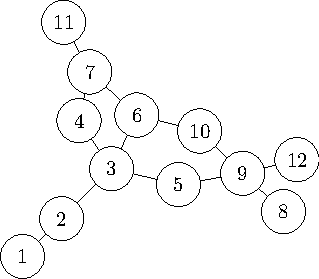
\includegraphics[width=0.65\textwidth]{chapters/gcol/figs/gheorghe-figure-2-figure0.pdf}
    \caption[A reproduction of the graph in Figure 2 of \cite{Gheorghe2013}]{\label{fig:gcol:gheorghefig2}A reproduction of Figure 2 from \cite{Gheorghe2013}.  Although this figure and Figure 2 in \cite{Gheorghe2013} are visually distinct, the graphs are isomorphic.}
\end{figure}

\begin{figure}
    \centering
    \begin{subfigure}[b]{0.35\textwidth}
        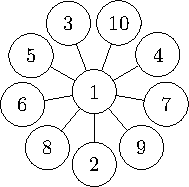
\includegraphics[width=\textwidth]{chapters/gcol/figs/g-10-1.pdf}
        \caption{\label{fig:gcol:g-10-1}\(G(10,1)\)}
    \end{subfigure}
    \hfill
    \begin{subfigure}[b]{0.35\textwidth}
        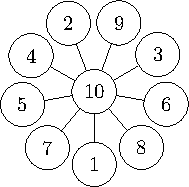
\includegraphics[width=\textwidth]{chapters/gcol/figs/g-10-10.pdf}
        \caption{\label{fig:gcol:g-10-10}\(G(10,10)\)}
    \end{subfigure}
    \caption[Graphs representing \(G(10,1)\) and \(G(10,10)\)]{\label{fig:gcol:gs}Graphs representing (a) \(G(10,1)\) and (b) \(G(10,10)\), as described in \cite{Gheorghe2013}, where the first number represents the size of the graph, and the second number represents the label of the centre node of the graph, with all other nodes connected only to that node.}
\end{figure}

\begin{figure}
    \centering
    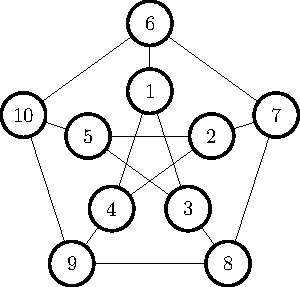
\includegraphics[width=0.45\textwidth]{chapters/gcol/figs/petersen-figure0.pdf}
    \caption[The Petersen Graph]{\label{fig:gcol:petersen}The classic Petersen graph, with nodes labelled 1 to 10.}
\end{figure}

Further simulations were run on complete graphs.  For a complete graph of \(N = 10\), the algorithm again required \qty{0.3}{\second}.  It was then tried on a complete graph of \(N = 20\), but the test had to be aborted after a matter of minutes due to the computer running out of memory.  Running times of \qty{0.83}{\second}, \qty{2.6}{\second}, \qty{8.88}{\second}, \qty{26.6}{\second} and \qty{84}{\second} for \(N = 11, 12, 13, 14\) and \(15\), respectively, were recorded.  Given that significant jumps in memory use were observed while running the larger graphs, it appears that the major cause of the rapid slowdown is likely to do with frequent \adhoc{} memory allocations and de-allocations, though this was not profiled in detail.

\citeauthor{Gheorghe2013} state \cite[p.~828]{Gheorghe2013} that in the latest version of \gls{plingua} at the time of writing, a strategy of eliminating \glspl{compartment} for which there can be no further rule applications is employed.  Using said strategy, results are typically achieved quite quickly.  It has the effect of pruning the search space, and reduces the total running time in some instances to just one-fifth of the running time of the simulation without such dead-\gls{compartment}-elimination.

The \fsharp{} program does not choose which \glspl{compartment} to operate upon in the same fashion, but applying the colour guard on rule \(r_{2,2n+1}\) of the \gls{skps}~system throughout the process results in the pruning of \glspl{compartment} which already contain invalid results and thus can be eliminated safely. Therefore, to achieve the same effect as with \gls{plingua}'s strategy, this guard was used while applying rule \(r_{2,2n+1}\) and the result used to filter out all invalid \glspl{compartment}.  Doing this reduces the evaluation of complete graphs to around 60 milliseconds or slightly more, since every \gls{compartment} in them can always be eliminated once colours have been assigned to four nodes.  It also reduces the running time of \cref{fig:gcol:gheorghefig2} to around \qty{0.25}{\second}, and the Petersen graph, \(G(10,1)\) and \(G(10,10)\) to \qty{0.1}{\second}.

\subsubsection{Comparison with Original Results}

\Cref{tab:gcol:timings} compares the timing results of the simulations reported in \cite{Gheorghe2013}, as well as the results of using \gls{mecosim}\footnote{The latest version of \gls{mecosim} available from \url{http://www.p-lingua.org/mecosim/} as at 10 January 2019 was used.} \cite{Perez-Hurtado2010} to re-run the same simulations locally on the same computer used to time the \fsharp{} solution, with the timing results mentioned above.

\begin{table}
\centering
\begin{tabular}{@{}lcccc@{}}
\toprule
Graph       & \begin{tabular}[c]{@{}c@{}}\gls{plingua}\\ (original)\end{tabular} & \begin{tabular}[c]{@{}c@{}}\gls{plingua}\\ (local)\end{tabular} & CML   & \begin{tabular}[c]{@{}c@{}}CML with\\ pruning\end{tabular} \\ \midrule
Fig. 2 in \cite{Gheorghe2013}      & N/A                                                           & 17.0                                                           & 2.6  & 0.25                                                 \\
Petersen    & N/A                                                           & 1.5                                                       & 0.3  & 0.1                                                       \\
G(10,1)     & 7                                                            & 2.6                                                           & 0.3  & 0.1                                                       \\
G(10,10)    & \textgreater 4 min                             & N/A                                                           & 0.3  & 0.1                                                       \\
Complete 11 & 5                                                            & 0.15                                                           & 0.83 & .06                                                       \\
Complete 12 & 5                                                            & 0.15                                                           & 2.6  & .06                                                       \\
Complete 13 & 5                                                            & 0.15                                                           & 8.88 & .06                                                       \\
Complete 14 & 5                                                            & 0.15                                                           & 26.6 & .06                                                       \\
Complete 15 & 5                                                            & 0.15                                                           & 84   & .06                                                       \\ \bottomrule
\end{tabular}%
\caption[Comparison of recorded timings between \cite{Gheorghe2013} and this work]{Comparison of recorded timings between \cite{Gheorghe2013} and this work.  All measurements are in seconds, unless otherwise stated.  Where more than one result was reported in \cite{Gheorghe2013} for the same graph, the shortest running time has been included here.}
\label{tab:gcol:timings}
\end{table}

Attempts to run the simulation of \(G(10,10)\) in \gls{mecosim} repeatedly failed with an out-of-memory error.  Why this should be the case is uncertain, given that in the other instances, executions of the \gls{mecosim} \gls{skps} simulations achieved lower runtimes than those of \cite{Gheorghe2013}.  The execution of \(G(10,10)\) notwithstanding, the overall improvements in runtime of the \glspl{skps} are likely due to a combination of the computer used locally being more recent and thus likely more powerful, and improvements in the underlying \gls{mecosim} and \gls{plingua} software.

It seems odd, however, that two functionally identical graphs, \(G(10,1)\) and \(G(10,10)\), would have such dramatically different run time behaviours when running in \gls{mecosim} --- seen in both the original and reproduced local results.  This might be due to an unusual performance bug hidden deep within \gls{mecosim}, though this was not investigated further.

These results appear to suggest that the \fsharp{} implementation generally provides superior running time results, though it was not tested on a particularly wide variety of scenarios.  Extrapolating from the collected results, it seems plausible that the scenarios that would result in the longest running time will likely be those that have a moderate level of connectedness in the graph.  Highly connected graphs will likely see many potential paths eliminated early due to frequent occurrences of colour conflicts, while graphs with few connections will have relatively few potential paths to explore.

The \fsharp{} results and those of the \gls{mecosim} simulations are not \emph{completely} comparable, however.  The \fsharp{} solution was programmed directly to follow the \gls{skps} system's rules, whereas the \gls{mecosim} solution was specified as the \gls{skps}~system rules in \gls{plingua}, with the operation of the computer simulation carried out by \gls{mecosim}.  This difference between `\adhoc{}' and `general' simulation means that one would expect to see the \fsharp{} simulation achieve better results from the outset, as overheads that accompany a general simulation implementation can be avoided.\footnote{One could see \adhoc{} as being akin to running a program compiled to native instructions, whereas using a general simulation is similar, in principle, to running a program in an interpreter.  The latter is typically simpler to work with and more portable, but comes with overheads that slow down execution.}  \Gls{mecosim} is an excellent tool, and, combined with \gls{plingua}, it provides a valuable service to the \gls{mc} community in that it allows researchers to validate their systems and \glspl{ruleset} while staying close to their mathematical descriptions, and without having to delve into the details of implementing a given algorithm in code.  See further \cite{Perez-Hurtado2019} for more of a discussion on \adhoc{} and general simulations, and a narrowing of the differences between the two.

Ultimately, this example is relatively trivial and involves little communication, and therefore does not test the use of \gls{cml} significantly.  Much of the operation of the algorithm in fact does not involve communication between different \glspl{compartment}/processing elements at all.  Instead, it is primarily based in the evolution of objects contained within the \glspl{compartment}, with minimal communication between \glspl{compartment} at the end.  While that is highly effective in \gls{ps} \cite{Paun2008}, it would be interesting to see the results of using \gls{cml} for other problems where synchronous communication\footnote{While \gls{cml} uses synchronous communication by default, it is also relatively simple to implement asynchronous communication also using it if desired \cite{Reppy2007}.} is a much bigger part of the evolution of the system.  The experimental results in \cref{chap:median} go some way to investigating this.

In common with most \adhoc{} simulations, while the implementation is reasonably successful, it is not particularly customisable, and the code as written does not comport as precisely to the appearance of the theoretical rules of the \gls{skps}~system as the \gls{plingua} version created for \cite{Gheorghe2013} does.  Neither does the current implementation have any form of verification or invariant detection, as provided by \gls{mecosim} \cite{Perez-Hurtado2010} and Spin \cite{Ben-Ari2008,Lefticaru2011}.

\gls{cml} seems to match to \gls{skps} well, but also looks like it might fit well with \gls{tlps} with symport/antiport \cite{Verlan2005} as well perhaps as \gls{tlps} with Channel States \cite{Song2016}, and Generalized Communicating \gls{ps} with minimal interaction rules \cite{Csuhaj-Varju2011}.  It would also appear to be a good fit for \gls{snps} \cite{Ionescu2006}, though \gls{cml} would probably be `overkill' for \gls{snps}.  In general, any variant of \gls{ps} which heavily uses synchronous communication between different cells/neurons/non-nested membranes/etc. over well-defined channels may be amenable to a \gls{cml} implementation.

Technically, the base form of \gls{cml} would only support symport (\ie{} one-way synchronous communication), but it is fairly simple to build two-way communication on top of it \cite[ch.~6]{Reppy2007}.  No attempt to model other systems has been made yet, however.
\section{\label{sec:gcol:cpsys}\glsentrytext{cps} solution to the \glsentrytext{gcp}}
In the \gls{cml} simulation of the problem, most of the work, in fact, is performed by the instantiation of new objects, rather than communication.  Thus, the problem appears to be an excellent fit to the pre-existing formulation of \gls{cps} \cite{Nicolescu2018}.

This solution assumes a graph with at most one edge between nodes (i.e. there are not two or more edges between the same two nodes), and that there are no edges leading from a node back to itself.  Further, it takes as given inputs to the process conceptual finite sets \(V \subset \mathbb{N}\) representing the nodes of the graph\footnote{In fact, any finite set of arbitrary symbols could be used, but this discussion is restricted to the natural numbers for ease of reading.}; \(E \subseteq \{(i,j)~|~i, j \in V, i \neq j \}\) representing the edges of the graph; and \(K\) representing the chosen colours, where \(K\) contains whatever representation of the desired colours is considered appropriate.

Based on these definitions, for the purposes of the remainder of this \namecref{chap:gcol}, \(|K|\) is defined to be the number of colours used in the current problem, \(|V|\) the number of nodes in the graph under consideration for the current problem and \(|E|\) the number of edges in the graph.

\subsection{Pseudocode for our parallel algorithm}
The logical operation of the system, as carried out using the rules described in detail at \cref{sec:gcol:rules}, can be demonstrated with a pseudocode representation, as shown in \cref{code:gcol:graphcol}.

% \begin{algorithm}
% \DontPrintSemicolon
% \SetKwFunction{Choose}{choose}
% \SetKwFunction{Dom}{Dom}
% \SetKwFunction{Graphcolouring}{Graph Colouring}
% \KwIn{\(V\), \(E\), \(K\)}
% \KwOut{A valid colouring, or an indication no valid colouring is possible}
% \Begin{
% \Choose{\(s \in V\), \(c \in K\)}\;
% \KwRet{\Graphcolouring{\(V\), \(E\), \(K\), \(1\), \(\{\{(s, c)\}\}\)}} \label{li:gcol:endofsmaller}
% }

% \hrulefill

% \KwIn{\(V\), \(E\), \(K\), \(i\), \(B\)}
% \KwOut{A valid colouring, or an indication no valid colouring is possible}
% \Begin{
% \If{\label{li:gcol:iflgreaterthanv} \(i = |V|\)} {
%     \Choose{\(m \in B\)}\;
%     \KwRet{\(m\)}    \label{li:gcol:returnsuccess}
% }
% \(B' \gets \emptyset\)\;
% \For{ \(m \in B,~x \in \Dom{m},~y \in V \setminus \Dom{m},~ d \in K \)}{    \label{li:gcol:makebstart}
%     \If{\((x,y) \in E ~ \land \not\exists(x',y) \in E,~(x',d) \in m\)}{
%         \(B' \gets B' \cup \{m \cup \{ (y,d) \} \}\)\;   \label{li:gcol:makebfinish}
%     }
% }
% \eIf{ \label{li:gcol:fail1} \(B' = \emptyset\) }
%   {
%         \KwRet{\(\emptyset\)}  \label{li:gcol:fail2}}
%     {
%         \KwRet{\Graphcolouring{\(V\), \(E\), \(K\), \(i + 1\), \(B'\)}\label{li:gcol:recurse}}
% }}
% \caption[Pseudocode representation of the algorithm performed by the \glspl{cps} rules in \cref{ruleset:gcol:rules}]{\label{code:gcol:graphcol}Pseudocode representation of the algorithm performed by the \glspl{cps} rules in \cref{ruleset:gcol:rules}.  This employs a doubly defined tail-recursive function approach, where the algorithm begins with the upper function supplied only with the details of the graph and colours, but uses the lower function with further arguments to perform most of the processing.}
% \end{algorithm}

\begin{algorithm}
\DontPrintSemicolon
\SetKwFunction{Choose}{choose}
\SetKwFunction{Dom}{Dom}
\SetKwFunction{Graphcolouring}{Graph Colouring}
\KwIn{\(V\), \(E\), \(K\)}
\KwOut{A valid colouring, or an indication no valid colouring is possible}
\Begin{
\Choose{\(s \in V\), \(c \in K\)}\;
\KwRet{\Graphcolouring{\(V\), \(E\), \(K\), \(\{\{(s, c)\}\}\)}} \label{li:gcol:endofsmaller}
}

\hrulefill

\KwIn{\(V\), \(E\), \(K\), \(B\)}
\KwOut{A valid colouring, or an indication no valid colouring is possible}
\Begin{
\If{\label{li:gcol:iflgreaterthanv} \(V = \emptyset\)} {
    \Choose{\(m \in B\)}\;
    \KwRet{\(m\)}    \label{li:gcol:returnsuccess}
}
\(B' \gets \emptyset\)\;
\For{ \(m \in B,~x \in \Dom{m},~y \in V \setminus \Dom{m},~ d \in K \)}{    \label{li:gcol:makebstart}
    \If{\((x,y) \in E ~ \land \not\exists(x',y) \in E,~(x',d) \in m\)}{
        \(B' \gets B' \cup \{m \cup \{ (y,d) \} \}\)\;   \label{li:gcol:makebfinish}
    }
}
\eIf{ \label{li:gcol:fail1} \(B' = \emptyset\) }
   {
        \KwRet{\(\emptyset\)}  \label{li:gcol:fail2}}
    {
        \KwRet{\Graphcolouring{\(V\), \(E\), \(K\), \(B'\)}\label{li:gcol:recurse}}
}}
\caption[Pseudocode representation of the algorithm performed by the \glspl{cps} rules in \cref{ruleset:gcol:rules}]{\label{code:gcol:graphcol}Pseudocode representation of the algorithm performed by the \glspl{cps} rules in \cref{ruleset:gcol:rules}.  This employs a doubly defined tail-recursive function approach, where the algorithm begins with the upper function supplied only with the details of the graph and colours, but uses the lower function with further arguments to perform most of the processing.}
\end{algorithm}

In our notation, \(m\) is a partial functional relation to \texttt{Dom}(m); \texttt{Dom}(m) is a partial spanning tree over the graph; \((x, c) \in m\) if and only if \(c\) is the colour of node \(x\);  and \(B\) is the set of all partial functional relations built up so far.

The system works by starting with the colours and graph under consideration, then building up, in a maximally-parallel fashion, a collection of objects which represent all validly coloured partial spanning trees of the graph.  Eventually, once full spanning trees have been constructed, one is chosen at random and its colouring output to the environment.  Or, if no valid colouring is possible, the system will detect that by the complete absence of any partial spanning tree, and signal to the environment that no appropriate colouring is possible.  The conceptual spanning trees are built following all possible tree edges, but checking that all new frond edges do not invalidate the colouring.

Note that while this algorithm is guaranteed to return a valid colouring if one is possible, there is \emph{no} guarantee as to precisely which valid colouring will be selected.  This \namecref{sec:gcol:cpsys} assumes that all potential colourings are equally desirable, and makes no provision for specifying that certain nodes must be coloured from a subset of the available colours.

\subsection{\label{sec:gcol:sysinit}\Glsfmtlongpl{cps} Initialisation}
System construction begins with a \gls{tlc} containing the functor \(V' = \cpset{\cpfunc{v}{\cpfunc{n}{i}} ~|~i \in V}\), which contains the labels of the nodes in \(V\); a set \(E' \subseteq \cpset{\cpfunc{e}{\cpfunc{n}{i} \, \cpfunc{n}{j}} ~|~(i,j) \in E}\) representing the edges of the graph; a starting node \(\cpfunc{s}{h}\) where \(h \in V\) is an arbitrary node label; and a set \(K' = \cpset{\cpfunc{k}{\kappa} ~|~ \kappa \in K}\) of  the potential colours.  In the case of the three-colour problem, it might look like \(K' = \cpset{\cpfunc{k}{r}, \cpfunc{k}{g}, \cpfunc{k}{b}}\). Using separate colour symbols in this fashion means that the algorithm can operate as a \(|K|\)-colour problem, without any other modification.

While colours are represented here as separate symbols for legibility, they can, in fact, be represented equivalently by natural numbers because each colour symbol is contained within a \(k\) functor --- one simply need fill each functor with the appropriate number of the counting symbol to represent the desired different colours.  E.g. \(r\) might be represented by one copy of the unary digit, \(\cpundig\), \(g\) by two and \(b\) by three, i.e. \(r = \cpfunc{k}{\cpundig}\), \(g = \cpfunc{k}{\cpundig^2}\) and \(b = \cpfunc{k}{\cpundig^3}\).  The same is true of the edges.  This means that, in fact, the system requires no extra symbols in its alphabet to represent the colours and edges of a given problem --- it merely re-uses atoms (see further in \cref{sec:gcol:notation}).

\subsection{\label{sec:gcol:notation}\Glsfmtlongpl{cps} Notation}
% \[
% cP\Pi(T, A, O, R, S, s_0)
% \]

% \(T\) is the set of \gls{tlc}s at the start of the evolution of the system; \(A\) is the alphabet of the system; \(O\) is the set of multisets of initial objects in the \gls{tlc}s; \(R\) is the set of rulesets for each \gls{tlc}, \(S\) is the set of possible states of the system, and \(s_0 \in S\) is the starting state of the system. Further, \(|T| = |O| = |R|\).

% \[
% cP\Pi(\{\sigma_1\}, A, \{O_1\}, \{r_1\}, S, s_1)
% \] where the set \(T = \{\sigma_1\}\) is the single \gls{tlc} of the system; \(A = \{b, c, e,\allowbreak l,\allowbreak m,\allowbreak n, s, v, k\} \allowbreak \cup \{\cpundig\}\) is all potential atoms, functors and other symbols of the system (\(\cpundig\) is used here as the counting symbol representing natural numbers); \(O_1 = \{s(h)\} \cup V' \allowbreak \cup E' \allowbreak \cup K'\) is the multiset of initial objects contained within \(\sigma_1\), where \(h\) is an arbitrarily chosen member of \(V\); \(R = \{r_1\}\) is the ruleset in \cref{ruleset:gcol:rules}; \(S = \{s_1, s_2, s_3, s_4\}\) is the potential states of the system; and \(s_1\) is the initial state of the system.

% In accordance with the \gls{cps} definition of \cref{sec:cps:formaldescriptions}, the \gls{gcp} \glspl{cps} can be formalised as \cptuple{g-col}{\cpset{\sigma_1}}{\cpset{b, c, e,\allowbreak l,\allowbreak m,\allowbreak n, s, v, k, \cpundig}}{\cpset{O_1}}{\cref{ruleset:gcol:rules}}{\cpset{s_1, s_2, s_3, s_4}}{s_1} where: the set \(T = \cpset{\sigma_1}\) is the single \gls{tlc} of the system; \(A = \cpset{b, c, e,\allowbreak l,\allowbreak m,\allowbreak n, s, v, k, \cpundig}\) is all potential atoms, functors and other symbols of the system; \(O_1 = \cpset{\cpfunc{s}{h}} \cup V' \allowbreak \cup E' \allowbreak \cup K'\) is the multiset of initial objects contained within \(\sigma_1\), where \(h\) is an arbitrarily chosen member of \(V\); \(R =\) \cref{ruleset:gcol:rules}.%; \(S = \cpset{s_1, s_2, s_3, s_4}\) is the potential states of the system; and \(s_1\) is the initial state of the system.

In accordance with the \gls{cps} definition of \cref{sec:cps:formaldescriptions}, the \gls{gcp} \glspl{cps} can be formalised as \cptuple{g-col}{\cpset{\sigma_1}}{\cpset{b, c, e,\allowbreak i,\allowbreak m,\allowbreak n, s, v, k, \cpundig}}{\cpset{O_1}}{\cref{ruleset:gcol:rules}}{\cpset{s_1, s_2, s_3, s_4}}{s_1} where: \(\sigma_1\) is the single \gls{tlc} of the system and \(O_1 = \cpset{\cpfunc{s}{h}} \cup V' \allowbreak \cup E' \allowbreak \cup K'\) is the multiset of initial objects contained within \(\sigma_1\), where \(h\) is an arbitrary member of \(V\).


\subsection{\label{sec:gcol:rules}Rules}

% \begin{cprulesetfloat}
% \begin{cpruleset}

%     \cprule{s_1}{\cpfunc{v}{\cpfunc{n}{S}Z}}\cponce{s_2}{\cpfunc{b}{\cpfunc{i}{\cpundig} \; \cpfunc{m}{\cpfunc{n}{S} \, \cpfunc{c}{C}} \; \cpfunc{v}{Z}} \; \cpfunc{i}{\cpundig}}
%     \cppromoter{\cpfunc{k}{C}}
%     \cppromoter{\cpfunc{s}{S}}
    
%     \cprule{s_2}{\cpfunc{b}{\cpfunc{i}{\cpdiscard} \; M \; \cpfunc{v}{\cpempty}}}\cponce{s_3}{\cpsend{M}{env}}
    
%     \cprule{s_2}{}\cpmaxpar{s_2}{\cpfunc{b}{\cpfunc{i}{I\cpundig} \; \cpfunc{m}{\cpfunc{n}{X} \, \cpfunc{c}{C}} \; \cpfunc{m}{\cpfunc{n}{Y} \, \cpfunc{c}{D}} \; M \; \cpfunc{v}{Z}}}
%     \cppromoter{\cpfunc{b}{\cpfunc{i}{I} \; \cpfunc{m}{\cpfunc{n}{X} \, \cpfunc{c}{C}} \; M \; \cpfunc{v}{\cpfunc{n}{Y}Z}}}
%     \cppromoter{\cpfunc{e}{\cpfunc{n}{X} \, \cpfunc{n}{Y}}}
%     \cppromoter{\cpfunc{k}{D}}
%     % \cpinhibitor{\{ \cpfunc{e}{\cpfunc{n}{X'} \, \cpfunc{n}{Y}} \land \cpfunc{m}{\cpfunc{n}{X'} \, \cpfunc{c}{D}} \}}
%     \cpinhibitor{\cpfunc{e}{\cpfunc{n}{X'} \, \cpfunc{n}{Y}} \lor \neg ~ \cpfunc{m}{\cpfunc{n}{X'} \, \cpfunc{c}{D}}}
    
%     \cprule{s_2}{\cpfunc{b}{\cpfunc{i}{I} \, \cpdiscard}}\cpmaxpar{s_2}{}
%     \cppromoter{\cpfunc{i}{I}}
    
%     \cprule{s_2}{}\cponce{s_4}{}
    
%     \cprule{s_2}{\cpfunc{i}{I}}\cponce{s_2}{\cpfunc{i}{I\cpundig}}

% \end{cpruleset}
% \caption[\gls{cps} rules for the \glsentrytext{gcp}]{\label{ruleset:gcol:rules}A completely generic \gls{cps} ruleset for solving the \gls{gcp}}
% \end{cprulesetfloat}

\begin{cprulesetfloat}
\begin{cpruleset}

    \cprule[rule:gcol:rules:init]{s_1}{\cpfunc{v}{\cpfunc{n}{S}Z}}\cponce{s_2}{\cpfunc{b}{\cpfunc{m}{\cpfunc{n}{S} \, \cpfunc{c}{C}} \; \cpfunc{v}{Z}} \; }
    \cppromoter{\cpfunc{k}{C}}
    \cppromoter{\cpfunc{s}{S}}
    
    \cprule[rule:gcol:rules:endsucc]{s_2}{\cpfunc{b}{M \; \cpfunc{v}{\cpempty}}}\cponce{s_3}{\cpsend{M}{env}}
    
    \cprule[rule:gcol:rules:loop]{s_2}{}\cpmaxpar{s_2}{\cpfunc{b}{\cpfunc{m}{\cpfunc{n}{X} \, \cpfunc{c}{C}} \; \cpfunc{m}{\cpfunc{n}{Y} \, \cpfunc{c}{D}} \; M \; \cpfunc{v}{Z}}}
    \cppromoter{\cpfunc{b}{\cpfunc{m}{\cpfunc{n}{X} \, \cpfunc{c}{C}} \; M \; \cpfunc{v}{\cpfunc{n}{Y}Z}}}
    \cppromoter{\cpfunc{e}{\cpfunc{n}{X} \, \cpfunc{n}{Y}}}
    \cppromoter{\cpfunc{k}{D}}
    % \cpinhibitor{\{ \cpfunc{e}{\cpfunc{n}{X'} \, \cpfunc{n}{Y}} \land \cpfunc{m}{\cpfunc{n}{X'} \, \cpfunc{c}{D}} \}}
    \cpinhibitor{\cpfunc{e}{\cpfunc{n}{X'} \, \cpfunc{n}{Y}} \lor \neg ~ \cpfunc{m}{\cpfunc{n}{X'} \, \cpfunc{c}{D}}}
    
    \cprule[rule:gcol:rules:loopclean]{s_2}{\cpfunc{b}{\cpdiscard}}\cpmaxpar{s_2}{}
    % \cppromoter{\cpfunc{i}{I}}
    
    \cprule[rule:gcol:rules:endfail]{s_2}{}\cponce{s_4}{}
    
    % \cprule{s_2}{\cpfunc{i}{I}}\cponce{s_2}{\cpfunc{i}{I\cpundig}}

\end{cpruleset}
\caption[\gls{cps} rules for the \glsentrytext{gcp}]{\label{ruleset:gcol:rules}A completely generic \gls{cps} ruleset for solving the \gls{gcp}}
\end{cprulesetfloat}

The rules are presented in \cref{ruleset:gcol:rules}.  The solution consists of six rules, which are invariant to the graph under consideration, and are listed in \emph{weak priority order}.  They are explained below:

\subsubsection{Description of rules}

\begin{enumerate}
\item This rule begins system evolution.  It converts the setup functor \(v\) into a functor \bo{}, which is used further to instantiate new objects with the possible colourings of the system.  It merely selects the node specified by the supplied \(s\) term, and assigns a colour at random.

The \bo{} object holds an \(i\) functor which keeps track of which iteration a given \bo{} belongs to; a multiset of \(m\) functors which track nodes and their assigned colours in a potential solution; and a \(v\) functor which continues to track the reducing unexplored nodes of the graph.

A separate global \(i\) functor is also instantiated at this point, which tracks the current iteration number of the system and which is used in later rules.  This rule begins in state \(s_1\) and ends in state \(s_2\).  This rule corresponds to the upper \texttt{Graph Colouring} function in \cref{code:gcol:graphcol}.

\item This rule is one of the potential end points of the evolution of the system.  If there are no further remaining nodes to explore, i.e. the \bo{} objects have empty \(v\) functors, then one of the \bo{}s is selected at random and the set \(M\) of \(m\) functors within said \bo{} which contain a solution to the colouring problem is output to the environment.  This rule begins in state \(s_2\) and ends in state \(s_3\).  State \(s_3\) is used to indicate to the environment that a solution has been found and the evolution of the system has terminated.  The change in state means that no other rule can be applied if this rule is applied.  This rule corresponds to \crefrange{li:gcol:iflgreaterthanv}{li:gcol:returnsuccess} of the lower \texttt{Graph Colouring} function in \cref{code:gcol:graphcol}.

\item This rule is arguably the heart of the process, and runs in maximally-parallel mode --- meaning that every possible exploration from the currently extant \bo{} objects is performed simultaneously.  In each application, for every pre-existing \bo{} object, new ones are generated with a random colouration assigned to an unexplored node, so long as there exists an edge between those nodes in the graph \emph{and} the selected colours are not the same \emph{and} there does not already exist another \(m\) object within the current \bo{} object that represents another node connected to the newly chosen node with the same colour.  It also increments the iteration counter within the \bo{} object.  This rule begins in state \(s_2\) and ends in state \(s_2\).  This rule corresponds to \crefrange{li:gcol:makebstart}{li:gcol:makebfinish} of the lower \texttt{Graph Colouring} function in \cref{code:gcol:graphcol}.

The interaction of the \(v\) objects in the output and the first promoter work in the same fashion as \(y \in V \setminus \texttt{Dom}(M)\) in the pseudocode of \cref{code:gcol:graphcol}.  That is, this rule selects an \(n\) inside the given \bo{}'s \(v\), but naturally avoids selecting an \(n\) that is already used in one of the \bo{}'s \(m\)s because they have already been removed from \(v\).

\item This rule is a `cleaning' rule, which removes all extant \bo{} objects with the current iteration count, thus keeping the working space relatively clean.  Recall that in \gls{ps}, rules are applied top-to-bottom in a  weak priority order.  This means that, while this rule will eliminate the \bo{} objects used by \cpruleref{rule:gcol:rules:loop} to instantiate the next generation, said objects will not be eliminated until immediately after the application of \cpruleref{rule:gcol:rules:loop} and thus the two rules do not cause conflicts.  This rule begins in state \(s_2\) and ends in state \(s_2\).

The operation of this rule occurs implicitly in the pseudocode, and does not have corresponding lines.  There is no reference to the current set of \bo{}s, \(B\), carried forward into the next call of the pseudocode function.  Instead, \(B\) is replaced with \(B'\) for the next execution of the function, and \(B\) will be cleaned up by the system in whichever way it clears away objects once all references to them have been dropped.

% \item This rule is the other possible termination rule.  It merely transitions to state \(s_4\), which is used to signal to the environment that no solution is possible.  The key to this rule is that, because it transitions to state \(s_4\), it is only applicable if none of the prior rules are.  This effectively means that it can only apply if all \bo{} objects have been removed from the system (because the presence of at least one \bo{} would mean that one of the prior rules will apply), indicating that every possible combination explored so far has already found a colouring conflict and thus there is no possible valid solution.  This rule begins in state \(s_2\) and ends in state \(s_4\).  This rule corresponds to lines \ref{li:gcol:fail1}-\ref{li:gcol:fail2} of the lower \texttt{Graph Colouring} function in \cref{code:gcol:graphcol}.

\item This rule is the other possible termination rule.  It merely transitions to state \(s_4\), which is used to signal to the environment that no solution is possible.  The key to this rule is that, because it transitions to state \(s_4\), it is only applicable if none of the prior rules are.  This effectively means that it can only apply if all \bo{} objects have been removed from the system (because the presence of at least one \bo{} would mean that one of the prior rules will apply), indicating that every possible combination explored so far has already found a colouring conflict and thus there is no possible valid solution.  This rule begins in state \(s_2\) and ends in state \(s_4\).  This rule corresponds to \crefrange{li:gcol:fail1}{li:gcol:fail2} of the lower \texttt{Graph Colouring} function in \cref{code:gcol:graphcol}.

% \item This rule merely increments the global iteration counter.  It is placed last so that the termination rules can trigger before it, as otherwise it will always be applicable while the system is in state \(s_2\).  This rule begins in state \(s_2\) and ends in state \(s_2\), and thus is applied simultaneously with rules 3 and 4.  This rule is implemented in the successive recursive calls of the lower \texttt{Graph Colouring} function in \cref{code:gcol:graphcol} at line \ref{li:gcol:recurse}.  As part of the recursive call the value for \(i\) in the next call is given as the current value of \(i\) plus one, i.e. \(i\) is incremented as part of the function call.
\end{enumerate}

\subsubsection{Definition of terms}
\paragraph{Atoms}
\begin{description}
\cptermdef{\cpempty}{The standard \gls{cps} ``empty'' term symbol.}
% \cptermdef{\cpundig}{The \gls{cps} unary digit.}
\end{description}

\paragraph{Functors}
\begin{description}
\cptermdef{b}{Node exploration term.  This is a collection term, which holds information pertaining to the iteration at which the term was generated, the nodes explored so far on this path and the colours assigned to each node, and the remaining unexplored nodes in the graph.}
\cptermdef{c}{Colouring assignment term.  Records the colour assigned to a node for a particular exploration}
\cptermdef{e}{Edge node.  Lists two locations in the graph, if they have an edge connecting them.}
\cptermdef{k}{Colour term.  Stores one of the colours potentially to be used in colouring the graph under study.}
% \cptermdef{i}{Iteration counter.  Counts how many steps there have been so far in the system's evolution.}
\cptermdef{m}{Explored node term.  Records a node which has been visited in this particular exploration of the graph, and which colour the node was assigned.}
\cptermdef{n}{Node term.  Merely records the label of a node.  Used as part of other terms in the rules.}
\cptermdef{s}{Starting node.  Stores the label of the intended root node of the exploration of the graph.}
\cptermdef{v}{Unexplored nodes term.  Holds \(n\) terms with the labels of all nodes in the graph as yet unexplored in that particular exploration of the graph.}
\end{description}

\paragraph{States}
\begin{description}
\cptermdef{s_1}{System starting state.  The node in the \(s\) term is given a random colouring, and exploration of the graph begins.}
\cptermdef{s_2}{Main loop state.  All exploration of the graph and assignation of potential colours to nodes occurs in this state.}
\cptermdef{s_3}{Result state.  The system ends in this state if a valid colouring has been found.}
\cptermdef{s_4}{Negative result state.  The system ends in this state if no valid colouring is possible.}
\end{description}

\subsection{\label{sec:gcol:termination}Termination and Correctness}
The behaviour of the system in regard to termination and correctness is examined below.  The discussion in this \namecref{sec:gcol:termination} assumes that the number of steps taken is tracked in a variable \(i\).  No such subcell appears in \cref{ruleset:gcol:rules} because the rules make no use of the step number.

\begin{lemma}\label{lemma:gcol:grow}
All \bo{} objects present in the \gls{tlc} hold a monotonically growing set \(M\) of \(m\) functors, which represent validly coloured partial spanning trees of the whole graph, and at step \(i \leq |V|\) in the evolution of the system, each partial spanning tree will have a length equal to \(i\).
\end{lemma}

\begin{proof}
% At step one, a single \bo{} object will have been created by operation of rule 1.  Contained within this \bo{} object is a single \(m\) functor, which pairs a node label with a colour label.  Thus, the size of \(M\), \(|M|=1\), \(m \in M\).

At step one, a single \bo{} object will have been created by operation of \cpruleref{rule:gcol:rules:init}.  Contained within this \bo{} object is a single \(m\) functor, which pairs a node label with a colour label.  Thus, the size of \(M\), \(|M| = 1\), \(m \in M\).

At step \(i > 1\), any pre-existing \bo{} objects are removed, but are replaced with new \bo{} objects which between them cover all possible valid coloured partial spanning trees rooted at the initial node so far, after adding one further \(m\) object to \(M\), so \(|M| \geq 2\).  Thus, at step two, the extant \bo{} objects will each contain two \(m\) functors, one describing the initial node, and the other describing another node of the graph that has been chosen at random from among those that have an edge in the graph connecting said node to the first node.  By operation of the same rule, the number of node labels contained inside the \(v\) functor, itself inside each \bo{} object, will decrease by one, and thus the number of remaining unexplored nodes inside it will be equal to \(|V| - i\).

At step 3, there will be three \(m\) objects inside each \bo{} object, where there are edges in the graph connecting the represented nodes.  Due to the maximally-parallel nature of \cpruleref{rule:gcol:rules:loop}, every possible partial spanning tree of size \(i\) rooted at the initial node will be represented in a \bo{} object at step \(i\).  Assuming that a colouring is possible, the system proceeds in the same fashion for each following step, until step \(i = |V| + 1\) when the \(M\) sets inside the \bo{} objects contain full spanning trees, and the \(v\) functors will be empty.

At that point, \cpruleref{rule:gcol:rules:loop} can no longer be applied (because there will no longer be any \(n\) functors inside the \(v\) functors).  More importantly, \cpruleref{rule:gcol:rules:endsucc}, which enjoys priority under the weak priority ordering, becomes applicable and is thus selected as the rule to apply, ending evolution of the system with one of the \(M\) colouring sets output to the environment.

If a colouring is not possible, then eventually every possible application of \cpruleref{rule:gcol:rules:loop} will be confounded by the inhibitor, leading to \cpruleref{rule:gcol:rules:loopclean} removing all \bo{} objects without any more replacing them.  At this point (which can itself potentially occur at step \(i = |V| + 1\), such as in the case of a 4-node complete graph with 3 colours), \cpruleref{rule:gcol:rules:endfail} will terminate evolution of the system.
\end{proof}

\begin{lemma}\label{lemma:gcol:determin}
In all cases, evolution of the system proceeds wholly deterministically between the first and final steps, exclusively.
\end{lemma}

\begin{proof}
Due to the nature of rules \cpruleref*{rule:gcol:rules:loop} and \cpruleref*{rule:gcol:rules:loopclean}, which are the only ones applied during the middle steps of the system's evolution, there is essentially no choice made at any point.  Rules \cpruleref*{rule:gcol:rules:loop} and \cpruleref*{rule:gcol:rules:loopclean} make a non-deterministic choice in an individual application of them, but the rules are applied in a maximally parallel fashion, meaning that all possible choices are selected simultaneously.  Thus, all valid choices are explored, while the inhibitor ensures that no invalid choices are possible.

% \cpRuleref{rule:gcol:rules:endfail} is also deterministic.  It can only be applied when there are no \bo{} objects inside the \gls{tlc}, and thus the decision of whether it is applied or not simply requires checking the truth or otherwise of a simple proposition.  Further, there is only one possible result from applying \cpruleref{rule:gcol:rules:endfail} -- transitioning the system to state \(s_4\) --, so there is no choice involved in its application.  This means that, in all cases where there is no valid colouring possible (and thus the system will end up in a state with no \bo{} objects), the final step of the system is also deterministic.

\cpRuleref{rule:gcol:rules:endfail} is also deterministic.  It applies if and only if none of the earlier rules are applicable.  Further, there is only one possible result from applying \cpruleref{rule:gcol:rules:endfail} -- transitioning the system to state \(s_4\) --, so there is no choice involved in its application.  This means that, in all cases where there is no valid colouring possible, the final step of the system is also deterministic.

% Likewise, rule 6 is deterministic, because there will only be one \(i\) functor contained within the \gls{tlc}.
\end{proof}

\begin{lemma}\label{lemma:gcol:nondet}
% The system is only non-deterministic regarding the choice of the colour of the starting node and the final selection of which valid colouring to send out to the environment, assuming that the evolution of the system finishes with an application of \cpruleref{rule:gcol:rules:endsucc}.

The system is only non-deterministic regarding the choice of the colour of the starting node and the final selection of which valid colouring to send out to the environment, assuming that the evolution of the system finishes in state \(s_3\).
\end{lemma}

\begin{proof}
The system is deterministic for all rule applications except the first, and potentially the last, by \cref{lemma:gcol:determin}.  Application of \cpruleref{rule:gcol:rules:init} to start the system is partially non-deterministic, specifically regarding the choice of the initial colour.  Application of \cpruleref{rule:gcol:rules:endsucc} to end the evolution of the system is likewise non-deterministic only in the choice of the set of colourings to send out.

\cpRuleref{rule:gcol:rules:init} uses the pre-selected starting node, encoded in the \(s\) functor, to create the first \bo{} object with which to evolve the system.  While that functor will be unique by the creation conditions described above,\footnote{Should it be desired, it would be possible to have the system make a random selection between possible starting nodes, simply by starting the system with more than one \(s\) functor.  The correctness and termination of the system will be unaffected.} it has a free choice between the available colours.  As the rule is applied exactly once due to its application mode, only one colour is selected, but the specification of the colour promoter for \cpruleref{rule:gcol:rules:init} simply states that one of the supplied \(k\) colour objects is used.

While this selection is non-deterministic, it has no impact upon the termination of the evolution of the system, because for the standard \gls{gcp} there is no functional difference between colours.  That is, they do not imbue special properties or behaviours to their marked nodes, they merely label them.  Thus, the colour selected does limit the potential colouring sets that are available at the end by fixing the colour of the starting node, but has no impact upon which rule is applied next.

Finally, as with the selection of a colour in \cpruleref{rule:gcol:rules:init}, the selection of which extant \bo{} object to take the colouring set \(M\) out of and send out to the environment by \cpruleref{rule:gcol:rules:endsucc} is non-deterministic, as \cpruleref{rule:gcol:rules:endsucc} has a free choice in which one it selects.  From its perspective, any \bo{} object with an empty \(v\) functor is acceptable.
\end{proof}

\begin{lemma}\label{lemma:gcol:ending}
The termination of the evolution of the system by application of \cpruleref{rule:gcol:rules:endsucc} or \cpruleref{rule:gcol:rules:endfail} is also deterministic.
\end{lemma}

\begin{proof}
Both \cpruleref{rule:gcol:rules:endsucc} and \cpruleref{rule:gcol:rules:endfail} can only be applied in specific, mutually exclusive circumstances.  In particular, it is only possible to apply \cpruleref{rule:gcol:rules:endsucc} when there is at least one \bo{} object, which additionally must have an empty \(v\) functor.  Conversely, \cpruleref{rule:gcol:rules:endfail} may only be applied where there are absolutely no extant \bo{} objects in the system.  The only way \bo{} objects can be removed is by operation of \cpruleref{rule:gcol:rules:loopclean}, which cannot be applied in the same step as either \cpruleref{rule:gcol:rules:endsucc} or \cpruleref{rule:gcol:rules:endfail}, as they have differing final states.  This means that \emph{only} one of \cpruleref{rule:gcol:rules:endsucc} or \cpruleref{rule:gcol:rules:endfail} may be applied during a step when either of them is applied, and both are considered to terminate the evolution of the system.  If there are any \bo{}s with an empty \(v\), then \cpruleref{rule:gcol:rules:endsucc} is applied.  If there are no \bo{}s whatsoever, then \cpruleref{rule:gcol:rules:endfail} is applied.  In all other cases after the first step, rules \cpruleref*{rule:gcol:rules:loop} and \cpruleref*{rule:gcol:rules:loopclean} are applied.
\end{proof}

\begin{theorem}
The evolution of every valid instance of this system (where the system is created in accordance with \cref{sec:gcol:notation}, and \(|V|, |E|, |K| > 0\)) will terminate, either sending a valid colouring out to the environment where a valid colouring is possible, or signalling by its state that no valid colouring is possible.
\end{theorem}

\begin{proof}
By \cref{lemma:gcol:determin,lemma:gcol:nondet} the applications of the rules are deterministic in all ways, except the choice of the colour of the starting node, and the choice of the final selected colouring.  Thus, the progression of the system is always deterministic.  By \cref{lemma:gcol:ending}, the evolution of the system is \emph{always} terminated by \cpruleref{rule:gcol:rules:endsucc} when there exist any \bo{} objects with a full set of colourings, or by \cpruleref{rule:gcol:rules:endfail} \emph{only} when no colouring is possible.  A full set of colourings inside a \bo{} is ensured under \cref{lemma:gcol:grow}.
\end{proof}

\subsection{\label{sec:gcol:complexity}Complexity}
This \namecref{sec:gcol:complexity} discusses the time and space complexity of the system, with an emphasis on the maximum for each because the minima are highly graph-dependent.

\subsubsection{Time Complexity}
The \glspl{cps} requires at most \(|V| + 1\) steps, where \(|V|\) is the total number of nodes in the graph.  In the successful case it will require that many, but for graphs where there is no possible \(|K|\)-colouring it may terminate early.

\cpRuleref{rule:gcol:rules:init} requires one application.  Rules \cpruleref*{rule:gcol:rules:endsucc} and \cpruleref*{rule:gcol:rules:endfail} between them require one application.  Rules \cpruleref*{rule:gcol:rules:loop} and \cpruleref*{rule:gcol:rules:loopclean} both require at most \(|V| - 1\) applications, but the applications occur concurrently in all cases because there is no chance for a conflict of states.  In total, that simplifies to at most \(|V| + 1\) steps, giving a time complexity of \bigoh{|V|}.  This holds regardless of the relative sizes of \(K\) and \(V\), as all possible valid colourings are simultaneously explored for a given node.  It is trivial to create a valid colouring when \(|V| \leq |K|\).   When \(|V| > |K|\), i.e., the number of nodes in the graph is at least one greater than the number of colours available, the maximally-parallel nature of \cpruleref{rule:gcol:rules:loop} ensures that the running time does not depend on \(|K|\).

Furthermore, in cases where \(|V| > |K|\) the system requires \emph{a minimum} of \(|K| + 2\) steps before terminating.  At each step up to step \(i = |K|\), it will always be possible to choose a colour that does not conflict with any chosen so far, simply by selecting a colour that has not been used yet.  

At step \(i = |K| + 1\), however, in the case of a complete graph, no further \bo{} objects can be created because no matter what colour is selected for the next node, it is guaranteed to conflict with one of the colours selected previously.  This means that \cpruleref{rule:gcol:rules:loopclean} will remove all current \bo{} objects, but \cpruleref{rule:gcol:rules:loop} does not replace them with new ones.  Thus, at the next step, \cpruleref{rule:gcol:rules:endfail} will transition the system to state \(s_4\), signalling to the environment that no colouring is possible, and the evolution of the system will terminate.  As such, a lower bound on the number of steps can be determined as \(|K| + 2\).  Other graphs may require more steps to reach an answer, but as described above, never more than \(|V| + 1\).

This is consistent with the upper bound, when \(|V|\) is strictly larger than \(|K|\).  \(|V|\) and \(|K|\) are both natural numbers, so the smallest possible difference between them is 1.  Thus, \(|K| + 1\) can be at most equal to \(|V|\), and therefore \(|K| + 2\) at most can be equal to \(|V| + 1\).  I.e.
\begin{align*}
    |K| &< |V|\\
    \implies |K| + 1 &\leq |V|\\
    \implies |K| + 2 &\leq |V| + 1
\end{align*}

Thus, the time complexity has an upper bound of \bigoh{|V|}, and a lower bound of \(\Omega(min(|K|, |V|))\).

\subsubsection{Space Complexity}
% The \emph{theoretical} maximum number of objects that can be present in the system at the end of each step from step 1 onwards is given by equation \eqref{eq:gcol:spacemax} below and provides an upper bound.

The \emph{theoretical} maximum number of objects that can be present in the system at the end of each step from step 1 onwards is given by \cref{eq:gcol:spacemax} below, which provides an exclusive upper bound.

% \begin{equation}\label{eq:gcol:spacemax}
%     \textsc{Space}_{\text{max}}(i) = \underbrace{\bigg(\frac{(|V| - 1)!}{(|V| - i)!} \times |K|^{i-1}\bigg)}_{b} + \underbrace{|K|}_{k} + \underbrace{|E|}_{e} + \underbrace{1}_{i}
% \end{equation}

\begin{equation}\label{eq:gcol:spacemax}
    \textsc{Space}_{\text{max}}(i) = \underbrace{\bigg(\frac{(|V| - 1)!}{(|V| - i)!} \times |K|^{i-1}\bigg)}_{b} + \underbrace{|K|}_{k} + \underbrace{|E|}_{e}
\end{equation}

The underbraces indicate what type of functor each part of the above counts inside the \gls{tlc}.  In practice, the system will \emph{never} contain this many objects at once, due to the restriction on creating new \bo{}s where there would be conflicting colours.  For the purposes of the above, \(0!\) (which will occur when \(i = |V|\)) is defined to be equal to 1.

After the first step, there will always be precisely one \bo{} object in the \gls{tlc}, simply by the operation of \cpruleref{rule:gcol:rules:init}, but in each proceeding step the count will depend on the exact nature of the graph and colour set under consideration.  At the point that \(i = |V| - 1\), for each \bo{} there will be only one possible choice for the next node to explore (as there will only be one \(n\) remaining in each \bo{}'s \(v\)), but each one of those choices can potentially be made with each one of the system's colours, and thus while the ``base'' number of \bo{}s will remain the same between those two steps, the total maximum possible number of \bo{}s will increase by a factor of \(|K|\).

A complete graph gives the upper limit to the number of objects that can exist, because (ignoring the operation of the inhibitor in \cpruleref{rule:gcol:rules:loop}) every node can be reached from any other given node, and thus it provides the widest possible search -- any non-complete graph will contain an incomplete set of edges between nodes, disallowing some potential explorations from taking place.  This gives an upper bound on space complexity proportional to the number of nodes and colours in the system under consideration, i.e. \(\mathcal{O}(|V||K|)\).  Of course, due to the operation of the inhibitor in \cpruleref{rule:gcol:rules:loop}, no more \bo{} objects will be created for a complete graph once \(i > |K|\).

% Equations \eqref{eq:gcol:wb} and \eqref{eq:gcol:w} provide formulae to calculate the total space requirements of an individual \bo{} and the overall system. These equations assume that the size of a functor that contains only atoms, such as the colour functors \(k\) which contain only a given number of the counting atom, is constant regardless of how many atoms it contains.  This is perhaps unrealistic in a real biological system, but is appropriate for computer simulations, where fixed-bit-length representations are likely used to represent the various elements of the system.

\Cref{eq:gcol:wb,eq:gcol:w} provide formulae to calculate the total space requirements of an individual \bo{} and the overall system. These equations assume that the size of a functor that contains only atoms, such as the colour functors \(k\) which contain only a given number of the counting atom, is constant regardless of how many atoms it contains.  This is perhaps unrealistic in a real biological system, but is appropriate for computer simulations, where fixed-bit-length representations are likely used to represent the various elements of the system.

% The size of each \bo{} can be described by \eqref{eq:gcol:wb}
% \begin{equation}\label{eq:gcol:wb}
%     s_b(b) = c_l + c_m |M| + (c_v + c_n |v|)
% \end{equation} where the various \(c_x\) terms are coefficients specifying the size of each type of object.  \(c_i\) represents the size of an \(i\) functors, \(c_n\) represents the size of \(n\) functors, \(c_k\) represents the size of \(k\) functors, \(c_m = c_n + c_k\), and \(|v|\) represents the number of nodes remaining in the \(v\) functor inside each \bo{}, while \(|M|\) similarly represents the number of \(m\) functors in each \bo{}.

The size of each \bo{} can be described by \cref{eq:gcol:wb}
\begin{equation}\label{eq:gcol:wb}
    s_b(b) = c_m |M| + (c_v + c_n) |v|
\end{equation} where the various \(c_x\) terms are coefficients specifying the size of each type of object.  \(c_n\) represents the size of \(n\) functors, \(c_k\) represents the size of \(k\) functors, \(c_m = c_n + c_k\), and \(|v|\) represents the number of nodes remaining in the \(v\) functor inside each \bo{}, while \(|M|\) similarly represents the number of \(m\) functors in each \bo{}.

% This in turn leads to \eqref{eq:gcol:w}, describing the size of the entire system.

% \begin{equation}\label{eq:gcol:w}
%     S = c_k |K| + c_e |E| + c_t + c_l + \sum_{b \in B}s_b(b)
% \end{equation} where \(c_e\) is the size of each edge object and \(c_t\) is the size of the \gls{tlc} itself.

This in turn leads to \cref{eq:gcol:w}, describing the size of the entire system.

\begin{equation}\label{eq:gcol:w}
    S = c_k |K| + c_e |E| + c_t + \sum_{b \in B}s_b(b)
\end{equation} where \(c_e\) is the size of each edge object and \(c_t\) is the size of the \gls{tlc} itself.

% If all the coefficients are assumed to be equal to 1, then \eqref{eq:gcol:wb} simplifies to 

% \begin{equation}
%     s_b(b) = |M| + 2 |v| + 1
% \end{equation}

% and \eqref{eq:gcol:w} to

% \begin{equation}
%     S = |K| + |E| + \sum_{b \in B}s_b(b) + 2
% \end{equation}

If all the coefficients are assumed to be equal to 1, then \cref{eq:gcol:wb} simplifies to 

\begin{equation}
    s_b(b) = |M| + 2 |v|
\end{equation}

and \cref{eq:gcol:w} to

\begin{equation}
    S = |K| + |E| + \sum_{b \in B}s_b(b) + 1
\end{equation}

\subsection{Comparison with the \texorpdfstring{\glsxtrlong{skps}}{Simple Kernel P systems} solution}
The \gls{cps} solution requires only five rules, which are \emph{invariant} to the problem graph under study, as opposed to defining a family of rules that are customised to the graph at hand.  Likewise for the alphabet.  The alphabet consists of only 9 functors and the \gls{cps} `empty' atom (\(\cpempty\)), but with the nesting of atoms and functors these combine into further forms.  As the semantic meaning of each never changes, this does not add a great deal of complexity.  The \gls{cps} solution requires roughly equivalent starting objects to the \gls{skps} solution.

\begin{table}
\begin{threeparttable}
\centering
\caption{\glsxtrlong{skps} vs. \gls{cps}}
\label{tab:gcol:skpcomp}
\begin{tabular}{@{}lcc@{}}
\toprule
Type/specification                & \gls{skps}        & \gls{cps} \\ \midrule
Alphabet                          & \(|V|(|V|-1)/2 + 7|V| + 10\) & \(10\)         \\
Rules                             & \(2|V|~\&~2|V| + 7\)       & 6          \\
Max. \# of subcompartments & \(3^|V| + 1\)             & N/A\tnote{a}          \\
Number of steps                   & \(2|V| + 3\)             & \(\leq |V| + 1\)         \\ \bottomrule
\end{tabular}%
\begin{tablenotes}
\item[a] \gls{cps} do not have a concept of subcompartments in the same way as \gls{skps}.  This distinction is discussed in \cref{sec:gcol:diffsubcomp}.
\end{tablenotes}
\end{threeparttable}
\end{table}


\Cref{tab:gcol:skpcomp} provides a comparison of the \gls{skps} solution presented in \cite{Gheorghe2013} compared with the solution presented above, and is based upon Table 1 in \cite{Gheorghe2013}.  

\subsubsection{\label{sec:gcol:diffsubcomp}Differing concepts of subcompartments}
Atoms are simple objects, but one could perhaps argue that functors should be regarded as somewhere between full subcompartments and simple objects because they are non-atomic and can potentially hold objects (including other functors) within themselves.  The key difference between subcompartments and functors is that the former have rules of their own and typically evolve separately to their containing compartment, whereas the latter have \emph{no} computing/evolutionary power of their own, and are simply nested objects operated upon by their \gls{tlc}'s rules.  A subcompartment could potentially have all its parent compartments removed and still function as though it now has the skin membrane, but not so functors.  This means that \gls{cps} does not have a concept of subcompartments completely comparable to \gls{skps}'s, with instead the functors in use being closer to normal inanimate objects.

\subsubsection{Rules length}
The `price' for reducing the number of rules and symbols involved in the system is arguably making the rules themselves more complex.\footnote{Though, arguably, these rules to be fairly easy to understand nevertheless --- they are simply longer and involve more symbols than those of other systems.}  Much the same as the \gls{skps}~system in \cite{Gheorghe2013} allows for a \enquote{more succinct (in terms of number of rules, objects, number of cells and execution steps)} specification than an earlier \gls{tlps} from \cite{Diaz-Pernil2008} ``at the expense of a greater length of the rules,'' so too does the \glspl{cps} again allow for a more compact solution to the problem in exchange for longer rules.

If one chooses to exclude the guards specified, then the longest rule in \cite{Gheorghe2013} has a length of \(5\).  Including the guards, however, (which seems more realistic), then the longest \gls{skps} rule has a length of \(3 + 3|V|(|V| - 1)/2\) while the longest rule in \cref{ruleset:gcol:rules}, \cpruleref{rule:gcol:rules:loop}, has a \emph{fixed} length of 14, determined by counting the number of distinct atoms, functors and variables that appear in it.  This is regarded as an acceptable price to pay, considering what this enables the system to achieve otherwise.  Which style is most appropriate fundamentally depends on the specifics of a given situation, and the relative costs of the alphabet size, rule length etc. in implementing a system in a chosen form.
\section{\label{sec:gcol:examples}Examples}

To demonstrate the operation of the \gls{cps} algorithm in a 3-colouring context, we provide a working example using the graph in \autoref{fig:gcol:examplegraph}, and a failing example where no successful 3-colouring is possible using the graph in \autoref{fig:gcol:examplegraphnosol}.

\begin{figure}
    \centering
    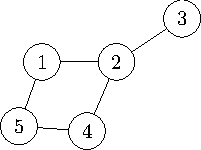
\includegraphics[width=0.4\textwidth]{chapters/gcol/figs/examplegraph1-figure2.pdf}
    \caption{Example undirected graph with at least one possible three-colouring solution (in fact, this graph is also potentially 2-colourable, and our \gls{cps} solution might select such a solution).}
    \label{fig:gcol:examplegraph}
\end{figure}

\begin{figure}
    \centering
    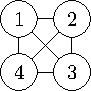
\includegraphics[width=0.2\textwidth]{chapters/gcol/figs/examplegraph1-figure3.pdf}
    \caption{Example undirected graph with no valid 3-colouring solutions.}
    \label{fig:gcol:examplegraphnosol}
\end{figure}

\subsection{Successful example}
For the graph in \autoref{fig:gcol:examplegraph}, we begin with a single top-level cell situated in the environment and in state \(s_0\).  From the hypothetical set of nodes \(V = \{1, 2, 3, 4, 5\}\) we derive the functor \(V' = \cpfunc{v}{\cpfunc{n}{1}~\cpfunc{n}{2}~\cpfunc{n}{3}~\cpfunc{n}{4}~\cpfunc{n}{5}}\), and the set of objects \[ 
E' = \{\cpfunc{e}{\cpfunc{n}{1} \, \cpfunc{n}{2}},~\cpfunc{e}{\cpfunc{n}{1} \, \cpfunc{n}{5}},~\cpfunc{e}{\cpfunc{n}{2} \, \cpfunc{n}{3}},~\cpfunc{e}{\cpfunc{n}{2} \, \cpfunc{n}{4}},~\cpfunc{e}{\cpfunc{n}{4} \, \cpfunc{n}{5}}\}
,\] representing the edges of the graph, as well as the set of colour objects \(K' = \{\cpfunc{k}{r},~\cpfunc{k}{g},~\cpfunc{k}{b}\}\), in this case representing the colours red, green and blue.  These sets of objects are all immediately within the top-level cell, along with \(\cpfunc{s}{1}\) to select node 1 at the beginning of the process, as shown in \autoref{objs:gcol:obj1}.

This beginning state, with the exception of the choice of node label inside the \(s\) object, is mandatory, but all following discussion in this subsection is merely one possible execution, due to the non-deterministic selection of colours that occurs during application of rule 1 and rule 2.

% \begin{figure}
% \begin{framed}
% \[
% e(\cpfunc{n}{1}\,\cpfunc{n}{2}) \quad \cpfunc{e}{\cpfunc{n}{1}\,\cpfunc{n}{5}} \quad \cpfunc{e}{\cpfunc{n}{2}\,\cpfunc{n}{3}} \quad \cpfunc{e}{\cpfunc{n}{2}\,\cpfunc{n}{4}} \quad \cpfunc{e}{\cpfunc{n}{4}\,\cpfunc{n}{5}}
% \]
% \[
% \cpfunc{k}{r} \quad \cpfunc{k}{g} \quad \cpfunc{k}{b} \quad \cpfunc{s}{1}\\
% \]
% \[
% \cpfunc{v}{\cpfunc{n}{1}~\cpfunc{n}{2}~\cpfunc{n}{3}~\cpfunc{n}{4}~\cpfunc{n}{5}}
% \]
% \end{framed}
% \caption{\label{fig:gcol:obj1}Initial set of objects inside the top-level cell for \autoref{fig:gcol:examplegraph}.}
% \end{figure}

\begin{cpobjectsfloat}
\begin{cpobjects}
\cpobjectsline{\cpfunc{e}{\cpfunc{n}{1} \, \cpfunc{n}{2}} \; \cpfunc{e}{\cpfunc{n}{1} \, \cpfunc{n}{5}} \; \cpfunc{e}{\cpfunc{n}{2} \, \cpfunc{n}{3}} \; \cpfunc{e}{\cpfunc{n}{2} \, \cpfunc{n}{4}} \; \cpfunc{e}{\cpfunc{n}{4} \, \cpfunc{n}{5}} \;}
% \[
% \cpfunc{e}{\cpfunc{n}{1}\,\cpfunc{n}{2}} \quad \cpfunc{e}{\cpfunc{n}{1}\,\cpfunc{n}{5}} \quad \cpfunc{e}{\cpfunc{n}{2}\,\cpfunc{n}{3}} \quad \cpfunc{e}{\cpfunc{n}{2}\,\cpfunc{n}{4}} \quad \cpfunc{e}{\cpfunc{n}{4}\,\cpfunc{n}{5}}
% \]
\cpobjectsline{ \cpfunc{k}{r} \; \cpfunc{k}{g} \; \cpfunc{k}{b} \quad \cpfunc{s}{1} \quad \cpfunc{v}{\cpfunc{n}{1} \; \cpfunc{n}{2} \; \cpfunc{n}{3} \; \cpfunc{n}{4} \; \cpfunc{n}{5}}}
% \[
% \cpfunc{k}{r} \quad \cpfunc{k}{g} \quad \cpfunc{k}{b} \quad \cpfunc{s}{1}\\
% \]
% \[
% \cpfunc{v}{\cpfunc{n}{1}~\cpfunc{n}{2}~\cpfunc{n}{3}~\cpfunc{n}{4}~\cpfunc{n}{5}}
% \]
\end{cpobjects}
\caption{\label{objs:gcol:obj1}Initial set of objects inside the top-level cell for \autoref{fig:gcol:examplegraph}.}
\end{cpobjectsfloat}

From this starting state, rule 1 is applied, choosing node 1 to start the process with, and selecting red as its colouring.  This creates the standard \(b\) and \(l\) objects.  No other rules are applicable at this point, as the top-level cell started in state \(s_0\).  The application of this rule leaves the top-level cell in state \(s_1\).  Rule 1 will henceforth be inapplicable, as the rules provide no way to revert to state \(s_0\).

% At the next step, rule 2 is checked but found inapplicable, as at this point the \(v\) object inside the only \(b\) object will not be empty, instead containing \(\cpfunc{v}{\cpfunc{n}{2}~ \cpfunc{n}{3}~ \cpfunc{n}{4}~ \cpfunc{n}{5}}\).  Rule 3, conversely, is applicable and thus can generate further new \(b\) objects.  In this instance, two edges exist from node 1 to other nodes (2 and 5 specifically), meaning that both choices can apply, generating new \(b\) objects containing all legal  colourings.  Both nodes are chosen to connect to, but there are only two other possible colourings to choose here, as red is currently blocked due to it being selected for the first \(b\) object.  This leads to the creation of four new \(b\) objects \(b\big(\cpfunc{l}{2}~\cpfunc{m}{\cpfunc{n}{1}\,\cpfunc{c}{r}}\allowbreak ~\cpfunc{m}{\cpfunc{n}{2}\,\cpfunc{c}{g}}\allowbreak ~\cpfunc{v}{\cpfunc{n}{3}~ \cpfunc{n}{4}~ \cpfunc{n}{5}}\big)\), \(b\big(\cpfunc{l}{2}~\cpfunc{m}{\cpfunc{n}{1}\,\cpfunc{c}{r}}\allowbreak ~\cpfunc{m}{\cpfunc{n}{5}\,\cpfunc{c}{b}}\allowbreak ~\cpfunc{v}{\cpfunc{n}{2}~ \cpfunc{n}{3}~ \cpfunc{n}{4}}\big)\) etc.

At the next step, rule 2 is checked but found inapplicable, as at this point the \(v\) object inside the only \(b\) object will not be empty, instead containing \(\cpfunc{v}{\cpfunc{n}{2}~ \cpfunc{n}{3}~ \cpfunc{n}{4}~ \cpfunc{n}{5}}\).  Rule 3, conversely, is applicable and thus can generate further new \(b\) objects.  In this instance, two edges exist from node 1 to other nodes (2 and 5 specifically), meaning that both choices can apply, generating new \(b\) objects containing all legal  colourings.  Both nodes are chosen to connect to, but there are only two other possible colourings to choose here, as red is currently blocked due to it being selected for the first \(b\) object.  This leads to the creation of four new \(b\) objects \(\cpfunc{b}{\cpfunc{l}{2}~\cpfunc{m}{\cpfunc{n}{1} \, \cpfunc{c}{r}}\allowbreak ~\cpfunc{m}{\cpfunc{n}{2} \, \cpfunc{c}{g}}\allowbreak ~\cpfunc{v}{\cpfunc{n}{3}~ \cpfunc{n}{4}~ \cpfunc{n}{5}}}\), \(\cpfunc{b}{\cpfunc{l}{2}~\cpfunc{m}{\cpfunc{n}{1} \, \cpfunc{c}{r}}\allowbreak ~\cpfunc{m}{\cpfunc{n}{5} \, \cpfunc{c}{b}}\allowbreak ~\cpfunc{v}{\cpfunc{n}{2}~ \cpfunc{n}{3}~ \cpfunc{n}{4}}}\) etc.

Simultaneously, rule 4 is applied to sweep away the pre-existing initial \(b\) object.  Rule 5 is not applicable because a state transition to state \(s_1\) has already been selected by application of rules 3 and 4, and thus a transition to state \(s_3\) is invalid.  Finally, rule 6 is also applied to remove the old \(l\) object and introduce a newly incremented one.  \autoref{objs:gcol:obj2} lists the objects in the top-level cell at the end of this step.

% \begin{figure}
% \begin{framed}
% \[
% e(\cpfunc{n}{1}\,\cpfunc{n}{2}) \quad \cpfunc{e}{\cpfunc{n}{1}\,\cpfunc{n}{5}} \quad \cpfunc{e}{\cpfunc{n}{2}\,\cpfunc{n}{3}} \quad \cpfunc{e}{\cpfunc{n}{2}\,\cpfunc{n}{4}} \quad \cpfunc{e}{\cpfunc{n}{4}\,\cpfunc{n}{5}}
% \]
% \[
%     \cpfunc{k}{r} \quad \cpfunc{k}{g} \quad \cpfunc{k}{b} \quad \cpfunc{l}{2}
% \]
% \[
% \cpfunc{b}{\cpfunc{l}{2}~\cpfunc{m}{\cpfunc{n}{1}\,\cpfunc{c}{r}}~\cpfunc{m}{\cpfunc{n}{2}\,\cpfunc{c}{g}}~\cpfunc{v}{\cpfunc{n}{3}~ \cpfunc{n}{4}~ \cpfunc{n}{5}}}
% \]
% \[
% \cpfunc{b}{\cpfunc{l}{2}~\cpfunc{m}{\cpfunc{n}{1}\,\cpfunc{c}{r}}~\cpfunc{m}{\cpfunc{n}{2}\,\cpfunc{c}{b}}~\cpfunc{v}{\cpfunc{n}{3}~ \cpfunc{n}{4}~ \cpfunc{n}{5}}}
% \]
% \[
% \cpfunc{b}{\cpfunc{l}{2}~\cpfunc{m}{\cpfunc{n}{1}\,\cpfunc{c}{r}}~\cpfunc{m}{\cpfunc{n}{5}\,\cpfunc{c}{g}}~\cpfunc{v}{\cpfunc{n}{2}~ \cpfunc{n}{3}~ \cpfunc{n}{4}}}
% \]
% \[
% \cpfunc{b}{\cpfunc{l}{2}~\cpfunc{m}{\cpfunc{n}{1}\,\cpfunc{c}{r}}~\cpfunc{m}{\cpfunc{n}{5}\,\cpfunc{c}{b}}~\cpfunc{v}{\cpfunc{n}{2}~ \cpfunc{n}{3}~ \cpfunc{n}{4}}}
% \]
% \end{framed}
% \caption{\label{fig:gcol:obj2}Set of objects inside the top-level cell after the second step (i.e. after one application of rules 3, 4 \& 6) for \autoref{fig:gcol:examplegraph}.}
% \end{figure}

\begin{cpobjectsfloat}
\begin{cpobjects}
\cpobjectsline{
\cpfunc{e}{\cpfunc{n}{1} \, \cpfunc{n}{2}} \; \cpfunc{e}{\cpfunc{n}{1} \, \cpfunc{n}{5}} \; \cpfunc{e}{\cpfunc{n}{2} \, \cpfunc{n}{3}} \; \cpfunc{e}{\cpfunc{n}{2} \, \cpfunc{n}{4}} \; \cpfunc{e}{\cpfunc{n}{4} \, \cpfunc{n}{5}}
}
\cpobjectsline{
    \cpfunc{k}{r} \; \cpfunc{k}{g} \; \cpfunc{k}{b} \quad \cpfunc{l}{2}
}
\cpobjectsline{
\cpfunc{b}{\cpfunc{l}{2}~\cpfunc{m}{\cpfunc{n}{1} \, \cpfunc{c}{r}}~\cpfunc{m}{\cpfunc{n}{2} \, \cpfunc{c}{g}}~\cpfunc{v}{\cpfunc{n}{3}~ \cpfunc{n}{4}~ \cpfunc{n}{5}}}
}
\cpobjectsline{
\cpfunc{b}{\cpfunc{l}{2}~\cpfunc{m}{\cpfunc{n}{1} \, \cpfunc{c}{r}}~\cpfunc{m}{\cpfunc{n}{2} \, \cpfunc{c}{b}}~\cpfunc{v}{\cpfunc{n}{3}~ \cpfunc{n}{4}~ \cpfunc{n}{5}}}
}
\cpobjectsline{
\cpfunc{b}{\cpfunc{l}{2}~\cpfunc{m}{\cpfunc{n}{1} \, \cpfunc{c}{r}}~\cpfunc{m}{\cpfunc{n}{5} \, \cpfunc{c}{g}}~\cpfunc{v}{\cpfunc{n}{2}~ \cpfunc{n}{3}~ \cpfunc{n}{4}}}
}
\cpobjectsline{
\cpfunc{b}{\cpfunc{l}{2}~\cpfunc{m}{\cpfunc{n}{1} \, \cpfunc{c}{r}}~\cpfunc{m}{\cpfunc{n}{5} \, \cpfunc{c}{b}}~\cpfunc{v}{\cpfunc{n}{2}~ \cpfunc{n}{3}~ \cpfunc{n}{4}}}
}
\end{cpobjects}
\caption{\label{objs:gcol:obj2}Set of objects inside the top-level cell after the second step (i.e. after one application of rules 3, 4 \& 6) for \autoref{fig:gcol:examplegraph}.}
\end{cpobjectsfloat}

The next step proceeds almost identically to the previous one, except that there are a greater number of new objects created (see \autoref{objs:gcol:obj3}).  At the previous step, the edges both between node 1 and node 5, and node 1 and node 2, were explored.  In this next step, edges between node 1 and node 5, node 1 and node 2 (where these edges were not explored previously for a given \(b\) object), node 5 and node 4, and node 2 and node 3 are all explored, with all objects that will not have direct colour conflicts instantiated as per rule 3.

% \begin{figure}
% \begin{framed}
% \begin{gather*}
%     \cpfunc{e}{\cpfunc{n}{1}\,\cpfunc{n}{2}} \quad \cpfunc{e}{\cpfunc{n}{1}\,\cpfunc{n}{5}} \quad \cpfunc{e}{\cpfunc{n}{2}\,\cpfunc{n}{3}} \quad \cpfunc{e}{\cpfunc{n}{2}\,\cpfunc{n}{4}} \quad \cpfunc{e}{\cpfunc{n}{4}\,\cpfunc{n}{5}}\\
%     \cpfunc{k}{r} \quad \cpfunc{k}{g} \quad \cpfunc{k}{b} \quad \cpfunc{l}{3}\\
%     \cpfunc{b}{\cpfunc{l}{3}~\cpfunc{m}{\cpfunc{n}{1}\,\cpfunc{c}{r}}~\cpfunc{m}{\cpfunc{n}{2}\,\cpfunc{c}{g}}~\cpfunc{m}{\cpfunc{n}{5}\,\cpfunc{c}{g}}~\cpfunc{v}{\cpfunc{n}{3}~ \cpfunc{n}{4}}} \\
%     \cpfunc{b}{\cpfunc{l}{3}~\cpfunc{m}{\cpfunc{n}{1}\,\cpfunc{c}{r}}~\cpfunc{m}{\cpfunc{n}{2}\,\cpfunc{c}{g}}~\cpfunc{m}{\cpfunc{n}{5}\,\cpfunc{c}{b}}~\cpfunc{v}{\cpfunc{n}{3}~ \cpfunc{n}{4}}} \\
%     \cpfunc{b}{\cpfunc{l}{3}~\cpfunc{m}{\cpfunc{n}{1}\,\cpfunc{c}{r}}~\cpfunc{m}{\cpfunc{n}{5}\,\cpfunc{c}{g}}~\cpfunc{m}{\cpfunc{n}{2}\,\cpfunc{c}{g}}~\cpfunc{v}{\cpfunc{n}{3}~ \cpfunc{n}{4}}} \\
%     \cpfunc{b}{\cpfunc{l}{3}~\cpfunc{m}{\cpfunc{n}{1}\,\cpfunc{c}{r}}~\cpfunc{m}{\cpfunc{n}{5}\,\cpfunc{c}{g}}~\cpfunc{m}{\cpfunc{n}{2}\,\cpfunc{c}{b}}~\cpfunc{v}{\cpfunc{n}{3}~ \cpfunc{n}{4}}} \\
%     \vdots\\
%     \cpfunc{b}{\cpfunc{l}{3}~\cpfunc{m}{\cpfunc{n}{1}\,\cpfunc{c}{r}}~\cpfunc{m}{\cpfunc{n}{2}\,\cpfunc{c}{b}}~\cpfunc{m}{\cpfunc{n}{3}\,\cpfunc{c}{r}}~\cpfunc{v}{\cpfunc{n}{4}~ \cpfunc{n}{5}}} \\
%     \cpfunc{b}{\cpfunc{l}{3}~\cpfunc{m}{\cpfunc{n}{1}\,\cpfunc{c}{r}}~\cpfunc{m}{\cpfunc{n}{2}\,\cpfunc{c}{b}}~\cpfunc{m}{\cpfunc{n}{3}\,\cpfunc{c}{g}}~\cpfunc{v}{\cpfunc{n}{4}~ \cpfunc{n}{5}}}
% \end{gather*}
% \end{framed}
% \caption{\label{fig:gcol:obj3}Set of objects inside the top-level cell after the third step for \autoref{fig:gcol:examplegraph}.  Note that there are some identical objects here which have been created independently.}
% \end{figure}

\begin{cpobjectsfloat}
\begin{cpobjects}
\begin{gather*}
    \cpfunc{e}{\cpfunc{n}{1} \, \cpfunc{n}{2}} \; \cpfunc{e}{\cpfunc{n}{1} \, \cpfunc{n}{5}} \; \cpfunc{e}{\cpfunc{n}{2} \, \cpfunc{n}{3}} \; \cpfunc{e}{\cpfunc{n}{2} \, \cpfunc{n}{4}} \; \cpfunc{e}{\cpfunc{n}{4} \, \cpfunc{n}{5}}\\
    \cpfunc{k}{r} \; \cpfunc{k}{g} \; \cpfunc{k}{b} \quad \cpfunc{l}{3}\\
    \cpfunc{b}{\cpfunc{l}{3}~\cpfunc{m}{\cpfunc{n}{1} \, \cpfunc{c}{r}}~\cpfunc{m}{\cpfunc{n}{2} \, \cpfunc{c}{g}}~\cpfunc{m}{\cpfunc{n}{5} \, \cpfunc{c}{g}}~\cpfunc{v}{\cpfunc{n}{3}~ \cpfunc{n}{4}}} \\
    \cpfunc{b}{\cpfunc{l}{3}~\cpfunc{m}{\cpfunc{n}{1} \, \cpfunc{c}{r}}~\cpfunc{m}{\cpfunc{n}{2} \, \cpfunc{c}{g}}~\cpfunc{m}{\cpfunc{n}{5} \, \cpfunc{c}{b}}~\cpfunc{v}{\cpfunc{n}{3}~ \cpfunc{n}{4}}} \\
    \cpfunc{b}{\cpfunc{l}{3}~\cpfunc{m}{\cpfunc{n}{1} \, \cpfunc{c}{r}}~\cpfunc{m}{\cpfunc{n}{5} \, \cpfunc{c}{g}}~\cpfunc{m}{\cpfunc{n}{2} \, \cpfunc{c}{g}}~\cpfunc{v}{\cpfunc{n}{3}~ \cpfunc{n}{4}}} \\
    \cpfunc{b}{\cpfunc{l}{3}~\cpfunc{m}{\cpfunc{n}{1} \, \cpfunc{c}{r}}~\cpfunc{m}{\cpfunc{n}{5} \, \cpfunc{c}{g}}~\cpfunc{m}{\cpfunc{n}{2} \, \cpfunc{c}{b}}~\cpfunc{v}{\cpfunc{n}{3}~ \cpfunc{n}{4}}} \\
    \vdots\\
    \cpfunc{b}{\cpfunc{l}{3}~\cpfunc{m}{\cpfunc{n}{1} \, \cpfunc{c}{r}}~\cpfunc{m}{\cpfunc{n}{2} \, \cpfunc{c}{b}}~\cpfunc{m}{\cpfunc{n}{3} \, \cpfunc{c}{r}}~\cpfunc{v}{\cpfunc{n}{4}~ \cpfunc{n}{5}}} \\
    \cpfunc{b}{\cpfunc{l}{3}~\cpfunc{m}{\cpfunc{n}{1} \, \cpfunc{c}{r}}~\cpfunc{m}{\cpfunc{n}{2} \, \cpfunc{c}{b}}~\cpfunc{m}{\cpfunc{n}{3} \, \cpfunc{c}{g}}~\cpfunc{v}{\cpfunc{n}{4}~ \cpfunc{n}{5}}}
\end{gather*}
\end{cpobjects}
\caption{\label{objs:gcol:obj3}Set of objects inside the top-level cell after the third step for \autoref{fig:gcol:examplegraph}.  Note that there are some identical objects here which have been created independently.}
\end{cpobjectsfloat}

At the fourth step, a large number of further objects are created, some of which are listed in \autoref{objs:gcol:obj4}.  The key difference between this step and the previous one is that the final inhibitor on rule 3 plays a much greater part.  At this step, many of the potential instantiations of new node and colouration selections will include conflicts between the newly-selected node and colour, and one or more of the node and colour selections made earlier.  The final inhibitor prevents instantiation of these choices, avoiding threats to correctness.  An alternative solution to the problem would be to include another following step, where those invalid instatiations are detected and removed, but the inhibitor makes this unnecessary.  

% \begin{figure}
% \begin{framed}
% \begin{gather*}
%     \cpfunc{e}{\cpfunc{n}{1}\,\cpfunc{n}{2}} \quad \cpfunc{e}{\cpfunc{n}{1}\,\cpfunc{n}{5}} \quad \cpfunc{e}{\cpfunc{n}{2}\,\cpfunc{n}{3}} \quad \cpfunc{e}{\cpfunc{n}{2}\,\cpfunc{n}{4}} \quad \cpfunc{e}{\cpfunc{n}{4}\,\cpfunc{n}{5}}\\
%     \cpfunc{k}{r} \quad \cpfunc{k}{g} \quad \cpfunc{k}{b} \quad \cpfunc{l}{4}\\
%     % \cpfunc{b}{\cpfunc{l}{3}~m(\cpfunc{n}{1}\,\cpfunc{c}{r}}~\cpfunc{m}{\cpfunc{n}{5}\,\cpfunc{c}{g}}~\cpfunc{m}{\cpfunc{n}{4}\,\cpfunc{c}{r}}~\cpfunc{v}{2~ 3}) \\
%     \cpfunc{b}{\cpfunc{l}{4}~\cpfunc{m}{\cpfunc{n}{1}\,\cpfunc{c}{r}}~\cpfunc{m}{\cpfunc{n}{5}\,\cpfunc{c}{g}}~\cpfunc{m}{\cpfunc{n}{4}\,\cpfunc{c}{r}}~\cpfunc{m}{\cpfunc{n}{2}\,\cpfunc{c}{g}}~\cpfunc{v}{\cpfunc{n}{3}}} \\
%     \cpfunc{b}{\cpfunc{l}{4}~\cpfunc{m}{\cpfunc{n}{1}\,\cpfunc{c}{r}}~\cpfunc{m}{\cpfunc{n}{5}\,\cpfunc{c}{g}}~\cpfunc{m}{\cpfunc{n}{4}\,\cpfunc{c}{r}}~\cpfunc{m}{\cpfunc{n}{2}\,\cpfunc{c}{b}}~\cpfunc{v}{\cpfunc{n}{3}}} \\
%     \cpfunc{b}{\cpfunc{l}{4}~\cpfunc{m}{\cpfunc{n}{1}\,\cpfunc{c}{r}}~\cpfunc{m}{\cpfunc{n}{5}\,\cpfunc{c}{g}}~\cpfunc{m}{\cpfunc{n}{4}\,\cpfunc{c}{r}}~\cpfunc{m}{\cpfunc{n}{2}\,\cpfunc{c}{g}}~\cpfunc{v}{\cpfunc{n}{3}}} \\
%     \cpfunc{b}{\cpfunc{l}{4}~\cpfunc{m}{\cpfunc{n}{1}\,\cpfunc{c}{r}}~\cpfunc{m}{\cpfunc{n}{5}\,\cpfunc{c}{g}}~\cpfunc{m}{\cpfunc{n}{4}\,\cpfunc{c}{r}}~\cpfunc{m}{\cpfunc{n}{2}\,\cpfunc{c}{b}}~\cpfunc{v}{\cpfunc{n}{3}}} \\
%     \vdots\\
%         \cpfunc{b}{\cpfunc{l}{4}~\cpfunc{m}{\cpfunc{n}{1}\,\cpfunc{c}{r}}~\cpfunc{m}{\cpfunc{n}{2}\,\cpfunc{c}{b}}~\cpfunc{m}{\cpfunc{n}{3}\,\cpfunc{c}{g}}~\cpfunc{m}{\cpfunc{n}{5}\,\cpfunc{c}{g}}~\cpfunc{v}{\cpfunc{n}{4}}} \\
%     \cpfunc{b}{\cpfunc{l}{4}~\cpfunc{m}{\cpfunc{n}{1}\,\cpfunc{c}{r}}~\cpfunc{m}{\cpfunc{n}{2}\,\cpfunc{c}{b}}~\cpfunc{m}{\cpfunc{n}{3}\,\cpfunc{c}{g}}~\cpfunc{m}{\cpfunc{n}{5}\,\cpfunc{c}{b}}~\cpfunc{v}{\cpfunc{n}{4}}}
% \end{gather*}
% \end{framed}
% \caption{\label{fig:gcol:obj4}Set of objects inside the top-level cell after the fourth step for \autoref{fig:gcol:examplegraph}.}
% \end{figure}  

\begin{cpobjectsfloat}
\begin{cpobjects}
\begin{gather*}
    \cpfunc{e}{\cpfunc{n}{1} \, \cpfunc{n}{2}} \; \cpfunc{e}{\cpfunc{n}{1} \, \cpfunc{n}{5}} \; \cpfunc{e}{\cpfunc{n}{2} \, \cpfunc{n}{3}} \; \cpfunc{e}{\cpfunc{n}{2} \, \cpfunc{n}{4}} \; \cpfunc{e}{\cpfunc{n}{4} \, \cpfunc{n}{5}}\\
    \cpfunc{k}{r} \; \cpfunc{k}{g} \; \cpfunc{k}{b} \quad \cpfunc{l}{4}\\
    % \cpfunc{b}{\cpfunc{l}{3}~m(\cpfunc{n}{1}\,\cpfunc{c}{r}}~\cpfunc{m}{\cpfunc{n}{5}\,\cpfunc{c}{g}}~\cpfunc{m}{\cpfunc{n}{4}\,\cpfunc{c}{r}}~\cpfunc{v}{2~ 3}) \\
    \cpfunc{b}{\cpfunc{l}{4}~\cpfunc{m}{\cpfunc{n}{1} \, \cpfunc{c}{r}}~\cpfunc{m}{\cpfunc{n}{5} \, \cpfunc{c}{g}}~\cpfunc{m}{\cpfunc{n}{4} \, \cpfunc{c}{r}}~\cpfunc{m}{\cpfunc{n}{2} \, \cpfunc{c}{g}}~\cpfunc{v}{\cpfunc{n}{3}}} \\
    \cpfunc{b}{\cpfunc{l}{4}~\cpfunc{m}{\cpfunc{n}{1} \, \cpfunc{c}{r}}~\cpfunc{m}{\cpfunc{n}{5} \, \cpfunc{c}{g}}~\cpfunc{m}{\cpfunc{n}{4} \, \cpfunc{c}{r}}~\cpfunc{m}{\cpfunc{n}{2} \, \cpfunc{c}{b}}~\cpfunc{v}{\cpfunc{n}{3}}} \\
    \cpfunc{b}{\cpfunc{l}{4}~\cpfunc{m}{\cpfunc{n}{1} \, \cpfunc{c}{r}}~\cpfunc{m}{\cpfunc{n}{5} \, \cpfunc{c}{g}}~\cpfunc{m}{\cpfunc{n}{4} \, \cpfunc{c}{r}}~\cpfunc{m}{\cpfunc{n}{2} \, \cpfunc{c}{g}}~\cpfunc{v}{\cpfunc{n}{3}}} \\
    \cpfunc{b}{\cpfunc{l}{4}~\cpfunc{m}{\cpfunc{n}{1} \, \cpfunc{c}{r}}~\cpfunc{m}{\cpfunc{n}{5} \, \cpfunc{c}{g}}~\cpfunc{m}{\cpfunc{n}{4} \, \cpfunc{c}{r}}~\cpfunc{m}{\cpfunc{n}{2} \, \cpfunc{c}{b}}~\cpfunc{v}{\cpfunc{n}{3}}} \\
    \vdots\\
        \cpfunc{b}{\cpfunc{l}{4}~\cpfunc{m}{\cpfunc{n}{1} \, \cpfunc{c}{r}}~\cpfunc{m}{\cpfunc{n}{2} \, \cpfunc{c}{b}}~\cpfunc{m}{\cpfunc{n}{3} \, \cpfunc{c}{g}}~\cpfunc{m}{\cpfunc{n}{5} \, \cpfunc{c}{g}}~\cpfunc{v}{\cpfunc{n}{4}}} \\
    \cpfunc{b}{\cpfunc{l}{4}~\cpfunc{m}{\cpfunc{n}{1} \, \cpfunc{c}{r}}~\cpfunc{m}{\cpfunc{n}{2} \, \cpfunc{c}{b}}~\cpfunc{m}{\cpfunc{n}{3} \, \cpfunc{c}{g}}~\cpfunc{m}{\cpfunc{n}{5} \, \cpfunc{c}{b}}~\cpfunc{v}{\cpfunc{n}{4}}}
\end{gather*}

\end{cpobjects}
\caption{\label{objs:gcol:obj4}Set of objects inside the top-level cell after the fourth step for \autoref{fig:gcol:examplegraph}.}
\end{cpobjectsfloat}

Step 5 proceeds analogously.  At the end of step 5 a number of \(b\) objects which contain valid colourings of the whole graph will be present inside the top-level cell.  At the sixth step, rule 2 will detect this by the fact that said objects will contain empty \(v\) functors.  For example, \autoref{objs:gcol:obj6} shows some of the potential solutions that could be generated, reflecting the state of the system at the end of the fifth step.  In fact, the first potential solution shows that in this case it is possible to completely and validly colour this graph using only two colours.  This solution may or may not be chosen when rule 2 is applied.  At the end of the sixth step, rule 2 will select one of the possible solutions and emit it to the environment.  The top-level cell will also transition to state \(s_2\), signalling that the process succeeded.

% \begin{figure}
% \begin{framed}
% \begin{gather*}
%     \cpfunc{e}{\cpfunc{n}{1}\,\cpfunc{n}{2}} \quad \cpfunc{e}{\cpfunc{n}{1}\,\cpfunc{n}{5}} \quad \cpfunc{e}{\cpfunc{n}{2}\,\cpfunc{n}{3}} \quad \cpfunc{e}{\cpfunc{n}{2}\,\cpfunc{n}{4}} \quad \cpfunc{e}{\cpfunc{n}{4}\,\cpfunc{n}{5}}\\
%     \cpfunc{k}{r} \quad \cpfunc{k}{g} \quad \cpfunc{k}{b} \quad \cpfunc{l}{5}\\
%     \cpfunc{b}{\cpfunc{l}{5}~\cpfunc{m}{\cpfunc{n}{1}\,\cpfunc{c}{r}}~\cpfunc{m}{\cpfunc{n}{5}\,\cpfunc{c}{g}}~\cpfunc{m}{\cpfunc{n}{4}\,\cpfunc{c}{r}}~\cpfunc{m}{\cpfunc{n}{2}\,\cpfunc{c}{g}}~\cpfunc{m}{\cpfunc{n}{3}\,\cpfunc{c}{r}}~v()} \\
%     \cpfunc{b}{\cpfunc{l}{5}~\cpfunc{m}{\cpfunc{n}{1}\,\cpfunc{c}{r}}~\cpfunc{m}{\cpfunc{n}{5}\,\cpfunc{c}{g}}~\cpfunc{m}{\cpfunc{n}{4}\,\cpfunc{c}{r}}~\cpfunc{m}{\cpfunc{n}{2}\,\cpfunc{c}{g}}~\cpfunc{m}{\cpfunc{n}{3}\,\cpfunc{c}{b}}~v()} \\
%             \vdots\\
%     \cpfunc{b}{\cpfunc{l}{5}~\cpfunc{m}{\cpfunc{n}{1}\,\cpfunc{c}{r}}~\cpfunc{m}{\cpfunc{n}{2}\,\cpfunc{c}{b}}~\cpfunc{m}{\cpfunc{n}{3}\,\cpfunc{c}{g}}~\cpfunc{m}{\cpfunc{n}{5}\,\cpfunc{c}{g}}~\cpfunc{m}{\cpfunc{n}{4}\,\cpfunc{c}{r}}~v()} \\
%     \cpfunc{b}{\cpfunc{l}{5}~\cpfunc{m}{\cpfunc{n}{1}\,\cpfunc{c}{r}}~\cpfunc{m}{\cpfunc{n}{2}\,\cpfunc{c}{b}}~\cpfunc{m}{\cpfunc{n}{3}\,\cpfunc{c}{g}}~\cpfunc{m}{\cpfunc{n}{5}\,\cpfunc{c}{g}}~\cpfunc{m}{\cpfunc{n}{4}\,\cpfunc{c}{r}}~v()}
% \end{gather*}
% \end{framed}
% \caption{\label{fig:obj6}Set of objects inside the top-level cell after the fifth step for \autoref{fig:gcol:examplegraph}.}
% \end{figure}

\begin{cpobjectsfloat}
\begin{cpobjects}

\begin{gather*}
    \cpfunc{e}{\cpfunc{n}{1} \, \cpfunc{n}{2}} \; \cpfunc{e}{\cpfunc{n}{1} \, \cpfunc{n}{5}} \; \cpfunc{e}{\cpfunc{n}{2} \, \cpfunc{n}{3}} \; \cpfunc{e}{\cpfunc{n}{2} \, \cpfunc{n}{4}} \; \cpfunc{e}{\cpfunc{n}{4} \, \cpfunc{n}{5}}\\
    \cpfunc{k}{r} \; \cpfunc{k}{g} \; \cpfunc{k}{b} \quad \cpfunc{l}{5}\\
    \cpfunc{b}{\cpfunc{l}{5}~\cpfunc{m}{\cpfunc{n}{1} \, \cpfunc{c}{r}}~\cpfunc{m}{\cpfunc{n}{5} \, \cpfunc{c}{g}}~\cpfunc{m}{\cpfunc{n}{4} \, \cpfunc{c}{r}}~\cpfunc{m}{\cpfunc{n}{2} \, \cpfunc{c}{g}}~\cpfunc{m}{\cpfunc{n}{3} \, \cpfunc{c}{r}}~v()} \\
    \cpfunc{b}{\cpfunc{l}{5}~\cpfunc{m}{\cpfunc{n}{1} \, \cpfunc{c}{r}}~\cpfunc{m}{\cpfunc{n}{5} \, \cpfunc{c}{g}}~\cpfunc{m}{\cpfunc{n}{4} \, \cpfunc{c}{r}}~\cpfunc{m}{\cpfunc{n}{2} \, \cpfunc{c}{g}}~\cpfunc{m}{\cpfunc{n}{3} \, \cpfunc{c}{b}}~v()} \\
            \vdots\\
    \cpfunc{b}{\cpfunc{l}{5}~\cpfunc{m}{\cpfunc{n}{1} \, \cpfunc{c}{r}}~\cpfunc{m}{\cpfunc{n}{2} \, \cpfunc{c}{b}}~\cpfunc{m}{\cpfunc{n}{3} \, \cpfunc{c}{g}}~\cpfunc{m}{\cpfunc{n}{5} \, \cpfunc{c}{g}}~\cpfunc{m}{\cpfunc{n}{4} \, \cpfunc{c}{r}}~v()} \\
    \cpfunc{b}{\cpfunc{l}{5}~\cpfunc{m}{\cpfunc{n}{1} \, \cpfunc{c}{r}}~\cpfunc{m}{\cpfunc{n}{2} \, \cpfunc{c}{b}}~\cpfunc{m}{\cpfunc{n}{3} \, \cpfunc{c}{g}}~\cpfunc{m}{\cpfunc{n}{5} \, \cpfunc{c}{g}}~\cpfunc{m}{\cpfunc{n}{4} \, \cpfunc{c}{r}}~v()}
\end{gather*}
\end{cpobjects}
\caption{\label{objs:gcol:obj6}Set of objects inside the top-level cell after the fifth step for \autoref{fig:gcol:examplegraph}.}
\end{cpobjectsfloat}

% ------------------------------------------------

\subsection{Failure example}
Here we step through the execution of the algorithm when there is no possible valid 3-colouring solution, using the graph depicted in \autoref{fig:gcol:examplegraphnosol}.  The system begins with the objects depicted in \autoref{objs:gcol:objn1}.

% \begin{figure}
% \begin{framed}
% \begin{gather*}
%     \cpfunc{e}{\cpfunc{n}{1}\,\cpfunc{n}{2}} \quad \cpfunc{e}{\cpfunc{n}{1}\,\cpfunc{n}{3}} \quad \cpfunc{e}{\cpfunc{n}{1}\,\cpfunc{n}{4}} \quad \cpfunc{e}{\cpfunc{n}{2}\,\cpfunc{n}{3}} \quad \cpfunc{e}{\cpfunc{n}{2}\,\cpfunc{n}{4}} \quad \cpfunc{e}{\cpfunc{n}{3}\,\cpfunc{n}{4}}\\
%     \cpfunc{k}{r} \quad \cpfunc{k}{g} \quad \cpfunc{k}{b} \quad \cpfunc{s}{1}\\
%     \cpfunc{v}{\cpfunc{n}{1}~\cpfunc{n}{2}~\cpfunc{n}{3}~\cpfunc{n}{4}}
% \end{gather*}
% \end{framed}
% \caption{\label{fig:objn1}Initial set of objects inside the top-level cell for \autoref{fig:gcol:examplegraphnosol}.}
% \end{figure}

\begin{cpobjectsfloat}
\begin{cpobjects}

\begin{gather*}
    \cpfunc{e}{\cpfunc{n}{1} \, \cpfunc{n}{2}} \; \cpfunc{e}{\cpfunc{n}{1} \, \cpfunc{n}{3}} \; \cpfunc{e}{\cpfunc{n}{1} \, \cpfunc{n}{4}} \; \cpfunc{e}{\cpfunc{n}{2} \, \cpfunc{n}{3}} \; \cpfunc{e}{\cpfunc{n}{2} \, \cpfunc{n}{4}} \; \cpfunc{e}{\cpfunc{n}{3} \, \cpfunc{n}{4}}\\
    \cpfunc{k}{r} \; \cpfunc{k}{g} \; \cpfunc{k}{b} \quad \cpfunc{s}{1}\\
    \cpfunc{v}{\cpfunc{n}{1}~\cpfunc{n}{2}~\cpfunc{n}{3}~\cpfunc{n}{4}}
\end{gather*}
\end{cpobjects}
\caption{\label{objs:gcol:objn1}Initial set of objects inside the top-level cell for \autoref{fig:gcol:examplegraphnosol}.}
\end{cpobjectsfloat}

After the first step, the application of rule 1, the objects shown in \autoref{objs:gcol:objn2} are inside the top-level cell.  This is not substantively different from the successful example above.  Likewise with the objects present in the cell at the end of the second step, shown in \autoref{objs:gcol:objn3}.

% \begin{figure}
% \begin{framed}
% \begin{gather*}
%     \cpfunc{e}{\cpfunc{n}{1}\,\cpfunc{n}{2}} \quad \cpfunc{e}{\cpfunc{n}{1}\,\cpfunc{n}{3}} \quad \cpfunc{e}{\cpfunc{n}{1}\,\cpfunc{n}{4}} \quad \cpfunc{e}{\cpfunc{n}{2}\,\cpfunc{n}{3}} \quad \cpfunc{e}{\cpfunc{n}{2}\,\cpfunc{n}{4}} \quad \cpfunc{e}{\cpfunc{n}{3}\,\cpfunc{n}{4}}\\
%     \cpfunc{k}{r} \quad \cpfunc{k}{g} \quad \cpfunc{k}{b} \quad \cpfunc{l}{1}\\
%     \cpfunc{b}{\cpfunc{l}{1}~\cpfunc{m}{\cpfunc{n}{1}\,\cpfunc{c}{r}}~\cpfunc{v}{\cpfunc{n}{2}~\cpfunc{n}{3}~\cpfunc{n}{4}}}
% \end{gather*}
% \end{framed}
% \caption{\label{fig:objn2}Set of objects inside the top-level cell at the end of step 1, for \autoref{fig:gcol:examplegraphnosol}.}
% \end{figure}

\begin{cpobjectsfloat}
\begin{cpobjects}

\begin{gather*}
    \cpfunc{e}{\cpfunc{n}{1} \, \cpfunc{n}{2}} \; \cpfunc{e}{\cpfunc{n}{1} \, \cpfunc{n}{3}} \; \cpfunc{e}{\cpfunc{n}{1} \, \cpfunc{n}{4}} \; \cpfunc{e}{\cpfunc{n}{2} \, \cpfunc{n}{3}} \; \cpfunc{e}{\cpfunc{n}{2} \, \cpfunc{n}{4}} \; \cpfunc{e}{\cpfunc{n}{3} \, \cpfunc{n}{4}}\\
    \cpfunc{k}{r} \; \cpfunc{k}{g} \; \cpfunc{k}{b} \quad \cpfunc{l}{1}\\
    \cpfunc{b}{\cpfunc{l}{1}~\cpfunc{m}{\cpfunc{n}{1} \, \cpfunc{c}{r}}~\cpfunc{v}{\cpfunc{n}{2}~\cpfunc{n}{3}~\cpfunc{n}{4}}}
\end{gather*}
\end{cpobjects}
\caption{\label{objs:gcol:objn2}Set of objects inside the top-level cell at the end of step 1, for \autoref{fig:gcol:examplegraphnosol}.}
\end{cpobjectsfloat}

% \begin{figure}
% \begin{framed}
% \begin{gather*}
%     \cpfunc{e}{\cpfunc{n}{1}\,\cpfunc{n}{2}} \quad \cpfunc{e}{\cpfunc{n}{1}\,\cpfunc{n}{3}} \quad \cpfunc{e}{\cpfunc{n}{1}\,\cpfunc{n}{4}} \quad \cpfunc{e}{\cpfunc{n}{2}\,\cpfunc{n}{3}} \quad \cpfunc{e}{\cpfunc{n}{2}\,\cpfunc{n}{4}} \quad \cpfunc{e}{\cpfunc{n}{3}\,\cpfunc{n}{4}}\\
%     \cpfunc{k}{r} \quad \cpfunc{k}{g} \quad \cpfunc{k}{b} \quad \cpfunc{l}{2}\\
%     \cpfunc{b}{\cpfunc{l}{2}~\cpfunc{m}{\cpfunc{n}{1}\,\cpfunc{c}{r}}~\cpfunc{m}{\cpfunc{n}{2}\,\cpfunc{c}{g}}~\cpfunc{v}{\cpfunc{n}{3}~\cpfunc{n}{4}}}\\
%     \cpfunc{b}{\cpfunc{l}{2}~\cpfunc{m}{\cpfunc{n}{1}\,\cpfunc{c}{r}}~\cpfunc{m}{\cpfunc{n}{2}\,\cpfunc{c}{b}}~\cpfunc{v}{\cpfunc{n}{3}~\cpfunc{n}{4}}}\\
%     \cpfunc{b}{\cpfunc{l}{2}~\cpfunc{m}{\cpfunc{n}{1}\,\cpfunc{c}{r}}~\cpfunc{m}{\cpfunc{n}{3}\,\cpfunc{c}{g}}~\cpfunc{v}{\cpfunc{n}{2}~\cpfunc{n}{4}}}\\
%     \cpfunc{b}{\cpfunc{l}{2}~\cpfunc{m}{\cpfunc{n}{1}\,\cpfunc{c}{r}}~\cpfunc{m}{\cpfunc{n}{3}\,\cpfunc{c}{b}}~\cpfunc{v}{\cpfunc{n}{2}~\cpfunc{n}{4}}}\\
%     \cpfunc{b}{\cpfunc{l}{2}~\cpfunc{m}{\cpfunc{n}{1}\,\cpfunc{c}{r}}~\cpfunc{m}{\cpfunc{n}{4}\,\cpfunc{c}{g}}~\cpfunc{v}{\cpfunc{n}{2}~\cpfunc{n}{3}}}\\
%     \cpfunc{b}{\cpfunc{l}{2}~\cpfunc{m}{\cpfunc{n}{1}\,\cpfunc{c}{r}}~\cpfunc{m}{\cpfunc{n}{4}\,\cpfunc{c}{b}}~\cpfunc{v}{\cpfunc{n}{2}~\cpfunc{n}{3}}}
% \end{gather*}
% \end{framed}
% \caption{\label{fig:objn3}Set of objects inside the top-level cell at the end of step 2, for \autoref{fig:gcol:examplegraphnosol}.}
% \end{figure}

\begin{cpobjectsfloat}
\begin{cpobjects}
\begin{gather*}
    \cpfunc{e}{\cpfunc{n}{1} \, \cpfunc{n}{2}} \; \cpfunc{e}{\cpfunc{n}{1} \, \cpfunc{n}{3}} \; \cpfunc{e}{\cpfunc{n}{1} \, \cpfunc{n}{4}} \; \cpfunc{e}{\cpfunc{n}{2} \, \cpfunc{n}{3}} \; \cpfunc{e}{\cpfunc{n}{2} \, \cpfunc{n}{4}} \; \cpfunc{e}{\cpfunc{n}{3} \, \cpfunc{n}{4}}\\
    \cpfunc{k}{r} \; \cpfunc{k}{g} \; \cpfunc{k}{b} \quad \cpfunc{l}{2}\\
    \cpfunc{b}{\cpfunc{l}{2}~\cpfunc{m}{\cpfunc{n}{1} \, \cpfunc{c}{r}}~\cpfunc{m}{\cpfunc{n}{2} \, \cpfunc{c}{g}}~\cpfunc{v}{\cpfunc{n}{3}~\cpfunc{n}{4}}}\\
    \cpfunc{b}{\cpfunc{l}{2}~\cpfunc{m}{\cpfunc{n}{1} \, \cpfunc{c}{r}}~\cpfunc{m}{\cpfunc{n}{2} \, \cpfunc{c}{b}}~\cpfunc{v}{\cpfunc{n}{3}~\cpfunc{n}{4}}}\\
    \cpfunc{b}{\cpfunc{l}{2}~\cpfunc{m}{\cpfunc{n}{1} \, \cpfunc{c}{r}}~\cpfunc{m}{\cpfunc{n}{3} \, \cpfunc{c}{g}}~\cpfunc{v}{\cpfunc{n}{2}~\cpfunc{n}{4}}}\\
    \cpfunc{b}{\cpfunc{l}{2}~\cpfunc{m}{\cpfunc{n}{1} \, \cpfunc{c}{r}}~\cpfunc{m}{\cpfunc{n}{3} \, \cpfunc{c}{b}}~\cpfunc{v}{\cpfunc{n}{2}~\cpfunc{n}{4}}}\\
    \cpfunc{b}{\cpfunc{l}{2}~\cpfunc{m}{\cpfunc{n}{1} \, \cpfunc{c}{r}}~\cpfunc{m}{\cpfunc{n}{4} \, \cpfunc{c}{g}}~\cpfunc{v}{\cpfunc{n}{2}~\cpfunc{n}{3}}}\\
    \cpfunc{b}{\cpfunc{l}{2}~\cpfunc{m}{\cpfunc{n}{1} \, \cpfunc{c}{r}}~\cpfunc{m}{\cpfunc{n}{4} \, \cpfunc{c}{b}}~\cpfunc{v}{\cpfunc{n}{2}~\cpfunc{n}{3}}}
\end{gather*}

\end{cpobjects}
\caption{\label{objs:gcol:objn3}Set of objects inside the top-level cell at the end of step 2, for \autoref{fig:gcol:examplegraphnosol}.}
\end{cpobjectsfloat}

\autoref{objs:gcol:objn4} shows the objects in the top-level cell at the end of step three.  This proceeds in much the same fashion as the previous step, but fully half of the potential instantiations from rule 3 are avoided by the rule's final inhibitor, due to inevitable colouration conflicts.

% \begin{figure}
% \begin{framed}
% \begin{gather*}
%     \cpfunc{e}{\cpfunc{n}{1}\,\cpfunc{n}{2}} \quad \cpfunc{e}{\cpfunc{n}{1}\,\cpfunc{n}{3}} \quad \cpfunc{e}{\cpfunc{n}{1}\,\cpfunc{n}{4}} \quad \cpfunc{e}{\cpfunc{n}{2}\,\cpfunc{n}{3}} \quad \cpfunc{e}{\cpfunc{n}{2}\,\cpfunc{n}{4}} \quad \cpfunc{e}{\cpfunc{n}{3}\,\cpfunc{n}{4}}\\
%     \cpfunc{k}{r} \quad \cpfunc{k}{g} \quad \cpfunc{k}{b} \quad \cpfunc{l}{3}\\
%     % \cpfunc{b}{\cpfunc{l}{2}~m(\cpfunc{n}{1}\,\cpfunc{c}{r}}~\cpfunc{m}{\cpfunc{n}{2}\,\cpfunc{c}{g}}~\cpfunc{v}{\cpfunc{n}{3}~\cpfunc{n}{4}})\\
%     \cpfunc{b}{\cpfunc{l}{3}~\cpfunc{m}{\cpfunc{n}{1}\,\cpfunc{c}{r}}~\cpfunc{m}{\cpfunc{n}{2}\,\cpfunc{c}{g}}~\cpfunc{m}{\cpfunc{n}{3}\,\cpfunc{c}{b}}~\cpfunc{v}{\cpfunc{n}{4}}}\\
%     \cpfunc{b}{\cpfunc{l}{3}~\cpfunc{m}{\cpfunc{n}{1}\,\cpfunc{c}{r}}~\cpfunc{m}{\cpfunc{n}{2}\,\cpfunc{c}{g}}~\cpfunc{m}{\cpfunc{n}{3}\,\cpfunc{c}{b}}~\cpfunc{v}{\cpfunc{n}{4}}}\\
%         \vdots\\
%     \cpfunc{b}{\cpfunc{l}{3}~\cpfunc{m}{\cpfunc{n}{1}\,\cpfunc{c}{r}}~\cpfunc{m}{\cpfunc{n}{2}\,\cpfunc{c}{g}}~\cpfunc{m}{\cpfunc{n}{4}\,\cpfunc{c}{b}}~\cpfunc{v}{\cpfunc{n}{3}}}\\
%     \cpfunc{b}{\cpfunc{l}{3}~\cpfunc{m}{\cpfunc{n}{1}\,\cpfunc{c}{r}}~\cpfunc{m}{\cpfunc{n}{2}\,\cpfunc{c}{g}}~\cpfunc{m}{\cpfunc{n}{4}\,\cpfunc{c}{b}}~\cpfunc{v}{\cpfunc{n}{3}}}
% \end{gather*}
% \end{framed}
% \caption{\label{fig:objn4}Set of objects inside the top-level cell at the end of step 3, for \autoref{fig:gcol:examplegraphnosol}.}
% \end{figure}

\begin{cpobjectsfloat}
\begin{cpobjects}

\begin{gather*}
    \cpfunc{e}{\cpfunc{n}{1} \, \cpfunc{n}{2}} \; \cpfunc{e}{\cpfunc{n}{1} \, \cpfunc{n}{3}} \; \cpfunc{e}{\cpfunc{n}{1} \, \cpfunc{n}{4}} \; \cpfunc{e}{\cpfunc{n}{2} \, \cpfunc{n}{3}} \; \cpfunc{e}{\cpfunc{n}{2} \, \cpfunc{n}{4}} \; \cpfunc{e}{\cpfunc{n}{3} \, \cpfunc{n}{4}}\\
    \cpfunc{k}{r} \; \cpfunc{k}{g} \; \cpfunc{k}{b} \quad \cpfunc{l}{3}\\
    % \cpfunc{b}{\cpfunc{l}{2}~m(\cpfunc{n}{1}\,\cpfunc{c}{r}}~\cpfunc{m}{\cpfunc{n}{2}\,\cpfunc{c}{g}}~\cpfunc{v}{\cpfunc{n}{3}~\cpfunc{n}{4}})\\
    \cpfunc{b}{\cpfunc{l}{3}~\cpfunc{m}{\cpfunc{n}{1} \, \cpfunc{c}{r}}~\cpfunc{m}{\cpfunc{n}{2} \, \cpfunc{c}{g}}~\cpfunc{m}{\cpfunc{n}{3} \, \cpfunc{c}{b}}~\cpfunc{v}{\cpfunc{n}{4}}}\\
    \cpfunc{b}{\cpfunc{l}{3}~\cpfunc{m}{\cpfunc{n}{1} \, \cpfunc{c}{r}}~\cpfunc{m}{\cpfunc{n}{2} \, \cpfunc{c}{g}}~\cpfunc{m}{\cpfunc{n}{3} \, \cpfunc{c}{b}}~\cpfunc{v}{\cpfunc{n}{4}}}\\
        \vdots\\
    \cpfunc{b}{\cpfunc{l}{3}~\cpfunc{m}{\cpfunc{n}{1} \, \cpfunc{c}{r}}~\cpfunc{m}{\cpfunc{n}{2} \, \cpfunc{c}{g}}~\cpfunc{m}{\cpfunc{n}{4} \, \cpfunc{c}{b}}~\cpfunc{v}{\cpfunc{n}{3}}}\\
    \cpfunc{b}{\cpfunc{l}{3}~\cpfunc{m}{\cpfunc{n}{1} \, \cpfunc{c}{r}}~\cpfunc{m}{\cpfunc{n}{2} \, \cpfunc{c}{g}}~\cpfunc{m}{\cpfunc{n}{4} \, \cpfunc{c}{b}}~\cpfunc{v}{\cpfunc{n}{3}}}
\end{gather*}
\end{cpobjects}
\caption{\label{objs:gcol:objn4}Set of objects inside the top-level cell at the end of step 3, for \autoref{fig:gcol:examplegraphnosol}.}
\end{cpobjectsfloat}

Finally, \autoref{objs:gcol:objn5} shows the objects in the top-level cell as at the end of step 4.  Due to the fully-connected nature of the graph in \autoref{fig:gcol:examplegraphnosol}, every possible solution will contain at least one instance of proposed contiguous colouration, thus making every possible solution invalid.  This means that rule 3 will not create any new \(b\) objects, while rule 4 will remove the pre-existing ones.

% \begin{figure}
% \begin{framed}
% \begin{gather*}
%     \cpfunc{e}{\cpfunc{n}{1}\,\cpfunc{n}{2}} \quad \cpfunc{e}{\cpfunc{n}{1}\,\cpfunc{n}{3}} \quad \cpfunc{e}{\cpfunc{n}{1}\,\cpfunc{n}{4}} \quad \cpfunc{e}{\cpfunc{n}{2}\,\cpfunc{n}{3}} \quad \cpfunc{e}{\cpfunc{n}{2}\,\cpfunc{n}{4}} \quad \cpfunc{e}{\cpfunc{n}{3}\,\cpfunc{n}{4}}\\
%     \cpfunc{k}{r} \quad \cpfunc{k}{g} \quad \cpfunc{k}{b} \quad \cpfunc{l}{4}
% \end{gather*}
% \end{framed}
% \caption{\label{fig:objn5}Set of objects inside the top-level cell at the end of step 4, for \autoref{fig:gcol:examplegraphnosol}.}
% \end{figure}

\begin{cpobjectsfloat}
\begin{cpobjects}

\begin{gather*}
    \cpfunc{e}{\cpfunc{n}{1} \, \cpfunc{n}{2}} \; \cpfunc{e}{\cpfunc{n}{1} \, \cpfunc{n}{3}} \; \cpfunc{e}{\cpfunc{n}{1} \, \cpfunc{n}{4}} \; \cpfunc{e}{\cpfunc{n}{2} \, \cpfunc{n}{3}} \; \cpfunc{e}{\cpfunc{n}{2} \, \cpfunc{n}{4}} \; \cpfunc{e}{\cpfunc{n}{3} \, \cpfunc{n}{4}}\\
    \cpfunc{k}{r} \; \cpfunc{k}{g} \; \cpfunc{k}{b} \quad \cpfunc{l}{4}
\end{gather*}
\end{cpobjects}
\caption{\label{objs:gcol:objn5}Set of objects inside the top-level cell at the end of step 4, for \autoref{fig:gcol:examplegraphnosol}.}
\end{cpobjectsfloat}

With no \(b\) objects available in the system, at the next step none of rules 1-4 will be applicable.  Thus, the first rule selected is rule 5, which merely transitions the top-level cell to state \(s_3\), signalling to the environment that the evolution of the system has ceased after determining that there was no possible valid colouring for the graph using the colours provided.

\section{\label{sec:gcol:conc}Conclusions}
Firstly, we implemented a version of \citeauthor{Gheorghe2013}'s \gls{skps} solution to the 3-colouring problem using \fsharp{} and a \gls{cml}-derived library, Hopac.   On the small sample of graphs tested, this produces reasonable results for smaller graphs, at least as good as those achieved by the \gls{plingua}/\gls{mecosim} simulation.  In both systems, the inclusion of a test for already-invalid compartments has the potential to improve the runtimes significantly, as it prunes the search space, sometimes quite dramatically.

\gls{cml} appears to be a good fit in principle to \gls{ps} variants that use communication between cells/membranes, but this particular problem had fairly minimal communication and instead relied heavily upon cell division.  Further testing with other problems is required to determine the efficacy of \gls{cml} for sure.

We secondly provided a single-top-level-cell \gls{cps} solution to the Graph Colouring Problem, which is capable of solving the problem for arbitrary graphs with an arbitrary number of potential colours in at most \(|V| + 1\) steps.  Its operation was demonstrated with two 3-colouring examples based on two different graphs, for which it was and was not possible, respectively, to find a valid 3-colouring.
